% Created with jtex v.1.0.20
\documentclass[a4paper,11pt,oneside]{book}
\usepackage[top=2cm, bottom=2cm, left=2cm, right=2cm]{geometry}
\usepackage[T1]{fontenc}
\usepackage[utf8]{inputenc}
\usepackage{lmodern}
\usepackage{graphicx}
\usepackage{caption}
\usepackage{natbib}
\usepackage{xcolor}
\usepackage{changepage}
\usepackage{framed}
\usepackage{hyperref}
\usepackage{amssymb}
\bibliographystyle{abbrvnat}

% Make list items more compact
\usepackage{enumitem}
\setlist[itemize]{noitemsep, topsep=0pt}

%%%%%%%%%%%%%%%%%%%%%%%%%%%%%%%%%%%%%%%%%%%%%%%%%%
%%%%%%%%%%%%%%%%%%%%  imports  %%%%%%%%%%%%%%%%%%%
\usepackage{amsmath}
\usepackage{amsthm}
\usepackage{booktabs}
\usepackage{url}
%%%%%%%%%%%%%%%%%%%%%%%%%%%%%%%%%%%%%%%%%%%%%%%%%%
%%%%%%%%%%%%%%%%%%%%%%%%%%%%%%%%%%%%%%%%%%%%%%%%%%
%%%%%%%%%%%%%%%%%%%%  theorem  %%%%%%%%%%%%%%%%%%%
\newtheorem{theorem}{Theorem}[section]
\newtheorem{corollary}{Corollary}[theorem]
\newtheorem{lemma}[theorem]{Lemma}
\newtheorem{proposition}{Proposition}[section]
\newtheorem{definition}{Definition}[section]
\newtheorem{example}{Example}[section]
\newtheorem{remark}{Remark}[section]
\newtheorem{axiom}{Axiom}[section]
\newtheorem{conjecture}{Conjecture}[section]
\newtheorem{observation}{Observation}[section]
%%%%%%%%%%%%%%%%%%%%%%%%%%%%%%%%%%%%%%%%%%%%%%%%%%




\hypersetup{
  colorlinks,
  linkcolor={black},
  citecolor={black},
  urlcolor={black}
}

% Style quotes
\definecolor{darkblue}{rgb}{0.0, 0.0, 0.55}
\definecolor{quoteshade}{rgb}{0.95, 0.95, 1}
\renewenvironment{quote}{%
  \def\FrameCommand{%
    \hspace{1pt}%
    {\color{darkblue}\vrule width 2pt}%
    {\color{quoteshade}\vrule width 4pt}%
    \colorbox{quoteshade}%
  }%
  \MakeFramed {\advance\hsize-\width \FrameRestore}%
  \noindent\hspace{-8pt}% disable indenting first paragraph
  \begin{adjustwidth}{0pt}{0pt}% adjust as needed
  \vspace{2pt}\vspace{2pt}%
}
{%
  \vspace{2pt}\end{adjustwidth}\endMakeFramed%
}

\title{\Huge \textbf{Matematične Tehnologije}}
\author{\textsc{Antonio Montero}}

\begin{document}
\sloppy

\frontmatter
\maketitle

\tableofcontents
% \listoffigures
% \listoftables

\mainmatter

% \include{preface.tex}
% \include{acknowledgements.tex}

\section{LaTeX}

\subsection{Uvod v LaTeX}

\subsubsection{Kaj je LaTeX?}\label{latexUvod_kajJeLaTeX}

LaTeX je program za oblikovanje besedil.
LaTeX je nadgradnja programa TeX, ki je razvil Donald E. Knuth. leta 1997.
Prvo verzijo LaTeX-a je napisal Leslie Lamport (1980). LaTeX je paket dodatnih ukazov za TeX, ki avtorjem omogočajo oblikovanje in izpisovanje dokumentov v najvišji kvaliteti s pomočjo že pripravljenih profesionalnih vzorcev.

Trenutna standardna verzija je LaTeX2e (1994), zanj pa je odgovoren Frank Mittelbach. LaTeX se izgovori `láteh', po angleško pa običajno rečemo `lejteh'.

Ko želi \textit{avtor} kaj objaviti, pošlje svoj rokopis založniku.
Tam \textit{knjiži opremljevalec} določi obliko dokumenta (širino stolpcev, obliko črk, velikost presledkov pred in po naslovih ... ).
Opremljevalec svoja navodila skupaj z rokopisom preda \textit{črkostavcu}, ki na podlagi teh podatkov stavi knjigo.
V LaTeX-u prevzame vlogi knjižnega oblikovalca in črkostavca, da se avtor osredotoči na vsebino Figure~\ref{kaj-je-latex}.

\begin{figure}[!htbp]
\centering
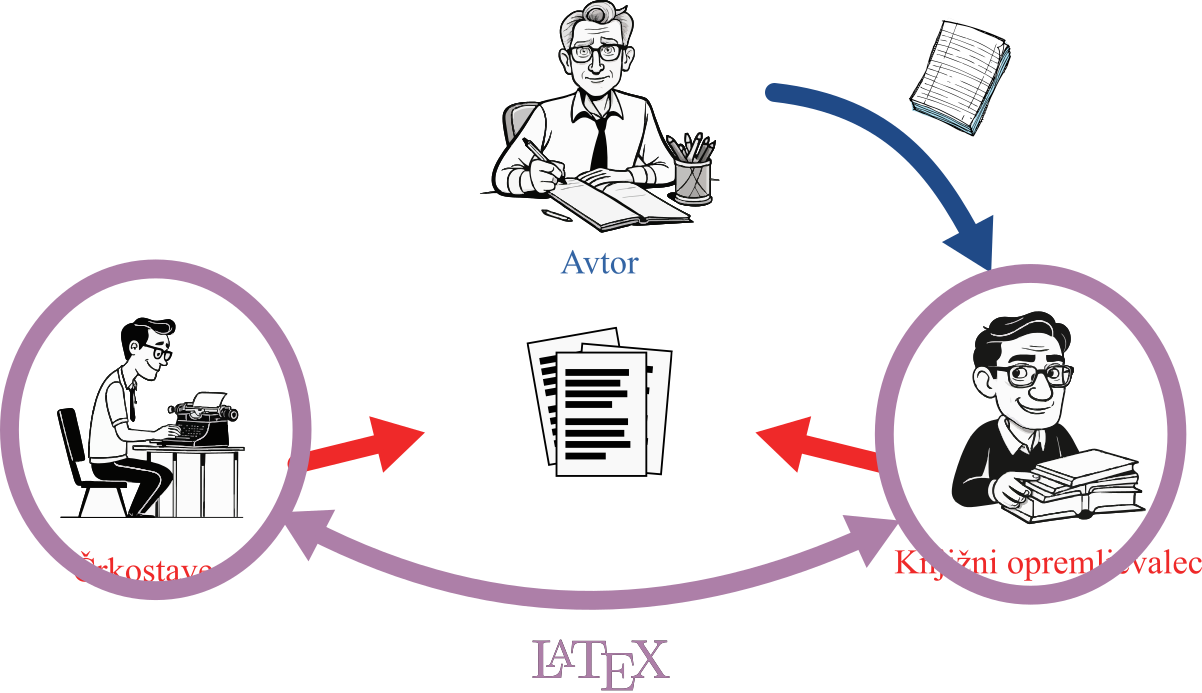
\includegraphics[width=0.8\linewidth]{files/01_osnovne-6aebd97826dc992bdf7f8e18b95c6a57.png}
\caption[]{Kaj je LaTeX?}
\label{kaj-je-latex}
\end{figure}

\begin{framed}
\textbf{Pomebno: Filozofija LaTeXa}\\
Oblikovanje dokumentov z LaTeXom sledi naslednjemu načelu:

\begin{quote}
mi (avtorji) se ukvarjamo z \textbf{vsebino} dokumenta, LaTeX pa poskrbi za \textbf{oblikovanje}.
\end{quote}

Ali, enakovredno,

\begin{quote}
ne skrbimo za \textbf{oblikovanje}, zato se lahko osredotočimo na \textbf{vsebino}.
\end{quote}
\end{framed}

\subsubsection{Kaj zmore LaTeX?}\label{latexUvod_KajZmoreLaTeX}

LaTeX zmore skoraj vse, kar zmorejo drugi urejevalniki besedil.
Vendar pa je LaTeX posebej primeren za pisanje znanstvenih in tehničnih besedil, ki vsebujejo veliko matematičnih formul in simbolov.
LaTeX omogoča tudi enostavno ustvarjanje tabel, grafov in drugih elementov, ki so pogosto potrebni v tehničnih besedilih.
Poleg tega LaTeX omogoča enostavno ustvarjanje kazal, bibliografij in drugih elementov, ki so pomembni za znanstvena besedila.

Čeprav je LaTeX optimiziran za izdelavo znanstvenih in tehničnih besedil, ni omejen samo na to. Danes uporabljam LaTeX za pisanje vseh dokumentov, ki naj izgledajo profesionalno ali lepo.
To sega od osebnih in poslovnih pisem do pesmarice za igranje kitare.

Vprašal sem moje sodelavce, kaj delajo z LaTeXom.
Tukaj je nekaj zanimivih odgovorov:

\begin{itemize}
\item Knjnige, članke, in zapiski predavanj;
\item Predstavitve, s pomočjo Beamer-ja \href{/latexbeamer}{Beamer: Prestavitve v LaTeXu};
\item Profesionalna dokumentacija (npr CV, projekte vloge);
\item Pogodbe za stanovanje;
\item Pisma;
\item Pravila za družabne igre
\item Note (za glasbo)
\item Facebook, SMS, Instagram (da, res je!).
\item \textbf{Zaključna dela (diplome, magistrska, doktorat)}
\end{itemize}

Če vas zanima, si lahko tukaj ogledate \href{https://anteromontonio.github.io/assets/pdf/2019\_Mon\_phDThesis.pdf}{mojo doktorsko disertacijo}, ki je bila napisana izključno z uporabo programa LaTeX.

\subsubsection{LaTeX ni Word}\label{latexUvod_latexNiWord}

MS Word, Google Docs, LibreOffice, so WYSIWYG (kar vidiš, to tudi dobiš).
V teh programih avtor obliko dokumenta določi interaktivno med samim vnosom besedila v računalnik. Med celotnim procesom na zaslonu vidi, kakšna bo končna oblika, ko bo dokument natisnjen.

Pri LaTeXu ni možno videti končne oblike med samim tipkanjem besedila.
Lahko pa vidimo končno obliko na zaslonu, potem ko datoteko prevedemo z LaTeXom.
Tako lahko popravke naredimo še preden dokument izpišemo s tiskalnikom.
V urejevalnikih WYSIWYG strukturo in obliko urejate hkrati z pisanjem besedila.
Zlasti pri dolgih projektih se je zelo lahko izgubiti.
LaTeX sili avtorja, da določi logično strukturo besedila, LaTeX pa potem izbere najprimernejšo obliko.

\paragraph{Zakaj LaTeX?}\label{latexUvod_zakaj}

Predstavljajmo si, da pišete roman v svojem najljubšem urejevalniku WYSIWYG.
V tej knjigi se odvijata dve vzporedni zgodbi v
različnih dimenzijah.
Da bi bralcu sporočili, katera od dimenzij je trenutno opisana, ste se odločili, da boste za obe uporabili različne barve.
Vaša knjiga bi tako lahko izgledala takole:

„Ne, ne moreš me zapustiti!`` je zaklical  Peredur Lancelotu.\newline
„Moram,`` je odgovoril. „Usoda me kliče. Toda ponovno se bova srečala. Obljubim.``

Shao je občutila nepojasnjeno žalost, kot da bi pravkar izgubila nekaj ali nekoga, ki ji je bil pomemben.\newline
„Si v redu?`` je vprašala Ashby, medtem ko je jedla svojo kašo.\newline
„Ne izgledaš dobro.``\newline
„V redu sem, samo utrujena.``

Ko ste končali prvi osnutek (ki obsega 300 strani), ste se odločili, da ga pošljete po e-pošti prijatelju, da vam bo povedal svoje mnenje.
Vendar se je izkazalo, da lahko tiskalnik vašega prijatelja tiska samo črno-belo, zato ne more natisniti datoteke, ki ste mu jo poslali.

Enostavna rešitev! Vse zeleno besedilo spremenite v kursivno pisavo, ostalo pa pustite v pisavi upright front.
Po ročni spremembi vsakega odstavka prvih 120 strani knjige ste se spomnili, da v nekaterih primerih za poudarjanje uporabljate kursivno pisavo:
[Ali boš \textit{to} jedla?]\{.latex-line .text-green\}
Sedaj boste morali preveriti vsak odstavek za kurzivo in ga spremeniti v drug slog, preden spremenite vse zeleno besedilo v kurzivo.

\textbf{Vidite neskončni problem?}.

LaTeX rešuje ta problem tako, da avtorju omogoča, da se osredotoči na vsebino in logično strukturo besedila, medtem ko LaTeX poskrbi za oblikovanje.

\subsubsection{Kako deluje LaTeX?}\label{latexUvod_kakoDeluje}

Klasična razlaga delovanja LaTeX-a je naslednja:

\begin{enumerate}
\item Avtor napiše besedilo in ukaze LaTeX v datoteko \texttt{.tex} (npr. \texttt{ime\_datoteke.tex}).
\item Datoteka \texttt{.tex} prevedemo z LaTeX-om, ki ustvari datoteko \texttt{.dvi} (npr. \texttt{ime\_datoteke.dvi}).
\item Datoteke \texttt{.dvi} niso standardne, zato je treba datoteka \texttt{.dvi} pogosto spremeniti v datoteko \texttt{.pdf}; na koncu dobimo datoteko \texttt{ime\_datoteke.pdf}, ki jo lahko natisnemo ali delimo z drugimi.
\end{enumerate}

V sodobnem času pogosto gremo iz \texttt{ime\_datoteke.tex} datoteke neposredno v \texttt{ime\_datoteke.pdf}\} npr. z pomočijo programa \texttt{pdflatex}.

\begin{figure}[!htbp]
\centering
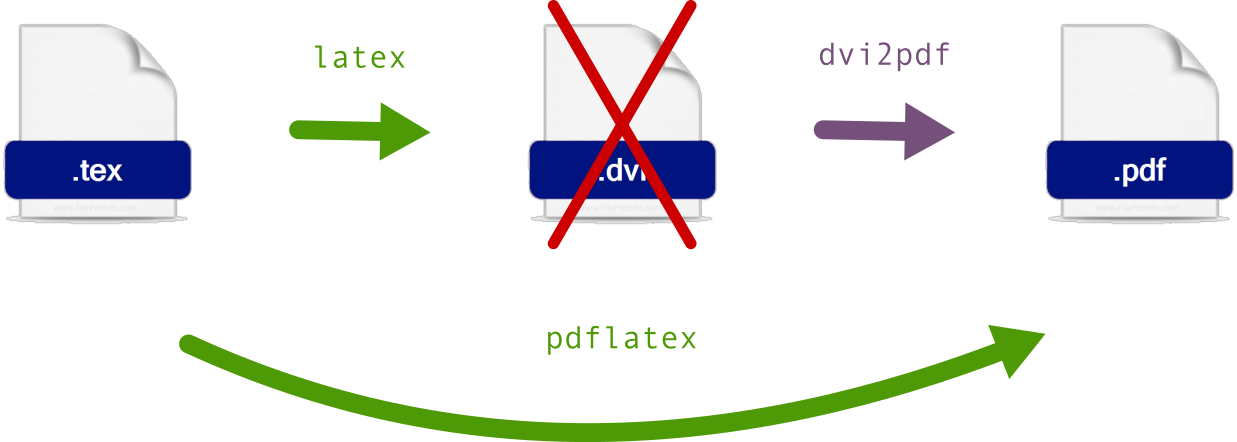
\includegraphics[width=0.8\linewidth]{files/01_datoteke-7b4841f3665416115ad84e4cf891a1cb.png}
\caption[]{Kajo deluje LaTeX?}
\label{kako-deluje-latex}
\end{figure}

\subsubsection{Kako začeti z LaTeXom?}\label{latexUvod_kakoZaceti}

Lahko namestite na svoj računalnik.
Če vas to želite, poglejte \href{/a-namescanjelatexa}{Nameščanje LaTeXa na svoj računalnik}.

Uporabili bomo drugačen pristop in delali z LaTeXom na spletu.
To bomo storili prek Overleaf, ki je platforma za delo z LaTeX projekti na spletu.
Najprej morate ustvariti račun.

%  ## Prva datoteka v LaTeXu

\subsubsection{Ukazi in okolja}

Kot smo že~omenili, se moramo pri delu z LaTeXom osredotočiti na vsebino, oblikovanje pa prepustiti LaTeXu.
Ker pa je LaTeX ``samo'' računalniški program, potrebuje
več vodenja.
Avtor mora navesti dodatne informacije, ki opisujejo logično strukturo njegovega dela.
Te informacije se navedejo prek \textit{ukazov} in \textit{okolij}, ki se vpišejo okoli besedila.

Ukazi v LaTeXu imajo splošno obliko:

\begin{verbatim}
\imeUkaza[neobvezni argument]{argument}
\end{verbatim}

in se običajno uporablja za dajanje LaTeXu določenih navodil.

\begin{itemize}
\item Ukaz \textit{vedno} se začne z znakom \texttt{{\textbackslash}}.
\item Argumentov je lahko več, npr. \texttt{\{prvi\}\{drugi\}...\{zadnji\}} ali  nobenega (npr. ukaz \texttt{{\textbackslash}tiny}, vendar je to redko).
\item Lahko je več neobveznih argumentov: \texttt{[prvi, drugi, ..., zadnji]}  ali noben (in potem ne napišemo ničesar). Pazite razliko z \texttt{obveznimi argumenti}.
\end{itemize}

Okolje je posebna vrsta ukaza z naslednjo strukturo:

\begin{verbatim}
\begin{okolje}
  Vsebina okolja: ukazi in besedilo
\end{okolje}
\end{verbatim}

Okolja običajno nadzorujejo, kako se bo del besedila/kode obnašal, ko bo natisnjen v dokument.

Zaenkrat vam ni treba skrbeti, kako delujejo ukazi in okolja.
To bomo spoznavali sproti.
V poglavju \href{/latexosnovnaokolja}{Osnovna okolja}  bomo podrobneje pogledali nekatera najpomembnejša okolja.

\subsubsection{Preambula in telo datoteke}\label{latexUvod_preambulaTelo}

Vsaka datoteka LaTeX ima naslednjo obliko:

\begin{verbatim}
%Preambula
\documentclass{...}
\usepackage{...}
%... 
% Telo
\begin{document}
  Vsebina dokumenta.
\end{document}
\end{verbatim}

Najpomembnejše okolje v lateksu je okolje \texttt{document}.
To okolje se lahko uporabi največ enkrat na dokument in v tem okolju pa napišemo dejansko vsebino našega dokumenta.
Vse, kar je znotraj tega okolja, se imenuje \textit{telo} dokumenta.

Če je najpomembnejše okolje \texttt{document}, mora biti najpomembnejši ukaz \texttt{{\textbackslash}documentclass}.
Vse, kar je med ukazom \texttt{{\textbackslash}documentclass} in začetkom okolja \texttt{document}, se imenuje \textit{preambula} dokumenta.
Tukaj nadzorujemo splošno delovanje LaTeXa.

\begin{framed}
\textbf{Opozirilo!}\\
Preambula običajno vsebuje samo ukaze (v nasprotju z običajnim besedilom) in obstajajo ukazi, ki se lahko uporabljajo samo v preambuli.
Pogosta napaka v LaTeXu je, da se del kode napiše na napačno mesto.
\end{framed}

Ukaz \texttt{{\textbackslash}documentclass} določa vrsto dokumenta, ki ga želimo ustvariti.
Uporabljamo ga tako

\begin{verbatim}
\documentclass[možnosti]{razred}
\end{verbatim}

Tu \texttt{razred} določa vrsto dokumenta, ki ga želimo ustvariti (npr. članek, knjiga, poročilo ...), \texttt{možnosti} pa so dodatne nastavitve, ki vplivajo na videz dokumenta (npr. velikost pisave, velikost papirja ...). V Table~\ref{tab_latex_razredi} so prikazani različni razredi dokumentov v LaTeXu.

\begin{table}
\centering
\caption[]{Razredi LaTeX dokumentov}
\label{tab_latex_razredi}
\begin{tabular}{p{\dimexpr 0.500\linewidth-2\tabcolsep}p{\dimexpr 0.500\linewidth-2\tabcolsep}}
\toprule
Razred & Opis \\
\hline
\texttt{article} & za članke v znanstvenih revijah, kratka poročila in druge krajše dokumente. \\
\texttt{proc} & razred za zbornike, ki temelji na razredu \textit{article}. \\
\texttt{report} & za daljša poročila, ki vsebujejo več poglavij, manjše knjige, doktorske disertacije, \dots \\
\texttt{book} & za prave knjige. \\
\texttt{beamer} & za predstavitve. \\
\texttt{letter} & za pisma. \\
\bottomrule
\end{tabular}
\end{table}

V tem učbeniku bomo obravnavali le razreda \texttt{article} in \texttt{beamer} (glej \href{/latexbeamer}{Beamer: Prestavitve v LaTeXu}, vendar bo večio tega, kar se bomo naučili, mogoče brez težav uporabiti tudi v drugih razredih.

Nekatere od uporabnih \texttt{možnosti} so \texttt{10pt} (prim. \texttt{11pt}, \texttt{12pt}), \texttt{a4paper} (prim. \texttt{letterpaper}), \texttt{onecolumn} (prim. \texttt{twocolumn}).
Privzete možnosti za \texttt{article} razred so \texttt{[letterpaper, 10pt, oneside, onecolumn, final]}.

\subsubsection{Avtor, naslov in datum}\label{latexUvod_avtorNaslovDatum}

Z ukazi \texttt{{\textbackslash}title}, \texttt{{\textbackslash}author} in \texttt{{\textbackslash}date} lahko določimo naslov, avtorja in datum dokumenta.
Ti ukazi se običajno uporabljajo v preambuli, vendar jih lahko uporabimo tudi v telesu dokumenta.
Ti ukazi ne ustvarijo ničesar, dokler ne uporabimo ukaza \texttt{{\textbackslash}maketitle}, ki ustvari naslovno stran z informacijami, ki smo jih določili z zgornjimi ukazi. Poglejte Example~\ref{eg-avtorNaslovDatum}.

\begin{example}\label{eg-avtornaslovdatum}\begin{verbatim}
% Preambula
% ...
\author{France Prešeren}
\title{Zdravljica}
\date{26.04.1848}    
% ... 
% Telo
\begin{document}
\maketitle
V tem dokumentu bom napisal ljubezensko pismo Juliji.
\end{document}
\end{verbatim}

\end{example}\subsubsection{Paketi in jeziki}\label{latexUvod_jezikPaketi}

LaTeX je zelo prilagodljiv in razširljiv sistem.
Osnovni LaTeX ponuja le osnovne funkcije, vendar lahko z uporabo \textit{paketov} dodamo nove funkcije in možnosti.
LaTeX ima okoli \href{https://www.ctan.org/pkg}{6000 paketov} na voljo.
Paketi so zbirke ukazov in okolij, ki jih lahko vključimo v naš dokument z ukazom

\begin{verbatim}
\usepackage{ime_paketa}.
\end{verbatim}

\begin{framed}
\textbf{Opozorilo!}\\
Ukaz \texttt{{\textbackslash}usepackage\{ime\_paketa\}} mora biti v preambuli, torej pred \texttt{{\textbackslash}begin\{document\}}.
\end{framed}

Eden najpomembnejših paketov je \texttt{babel}, ki omogoča uporabo različnih jezikov.
Paket naložimo z ukazom

\begin{verbatim}
\usepackage[jezik]{babel}
\end{verbatim}

kjer \texttt{jezik} določa jezik, ki ga želimo uporabiti (npr. \texttt{slovene}, \texttt{english}, \texttt{spanish}, \texttt{french}, \texttt{german}, \texttt{italian}, ...).
Paket \texttt{babel} poskrbi za pravilno oblikovanje besedila glede na izbrani jezik (npr. vezaje, ločila, datum, ...).

\begin{framed}
\textbf{Opomba!}\\
\begin{itemize}
\item V starih različicah LaTeXa nismo mogli preprosto pisati \textbf{č}, \textbf{š}, \textbf{ž}, \textbf{á}, \textbf{ü} \dots
\item Te črke lahko vedno dobimo z ukazi, kot so:
\end{itemize}

% \begin{table}
% % \centering
% \begin{tabular}{p{\dimexpr 0.500\linewidth-2\tabcolsep}p{\dimexpr 0.500\linewidth-2\tabcolsep}}
% \toprule
% Ukaz & Rezultat \\
% \hline
% \texttt{{\textbackslash}v\{c\}} & č \\
% \texttt{{\textbackslash}v\{s\}} & š \\
% \texttt{{\textbackslash}v\{z\}} & ž \\
% \texttt{{\textbackslash}'\{a\}} & á \\
% \texttt{{\textbackslash}"\{u\}} & ü \\
% \bottomrule
% \end{tabular}
% \end{table}

\begin{itemize}
\item Alternativno lahko uporabimo naslednje pakete za kodiranje znakov:
\end{itemize}

\begin{verbatim}
% Vhodnega dokumenta, 
\usepackage[utf8x]{inputenc} 
% opcije lahko so [utf8], [utf8x], ali [cp1215] 

% izhodnega dokumenta, 
\usepackage[T1]{fontenc} 
% lahko damo tudi [T2A] za cirilica
\end{verbatim}

\begin{itemize}
\item Sodobni LaTeX običajno ne potrebuje teh paketov.
Ponavadi je dovolj če uporabimo paket \texttt{babel}.
\end{itemize}
\end{framed}

\subsubsection{Komentarji, posbeni znaki, prazne vrstice in presledki.}\label{latexUvod_komentari}

\begin{framed}
\textbf{Nasvet!}\\
Pri delu v LaTeXu besedila \textbf{ne brišemo}, temveč ga \textbf{komentiramo}.
\end{framed}

Če želimo izpizati simbol \%, zapišemo \texttt{{\textbackslash}\%}.
Simbol \% je v LaTeXu poseben znak, to pomeni, da ima poseben pomen in ga ne moremo uporabiti kar tako.
Drugi posebni znaki v LaTeXu so prikazni v Table~\ref{tab-posebniZnaki}.

\begin{table}
\centering
\caption[]{Posebni znaki v LaTeXu}
\label{tab-posebniZnaki}
\begin{tabular}{p{\dimexpr 0.500\linewidth-2\tabcolsep}p{\dimexpr 0.500\linewidth-2\tabcolsep}}
\toprule
Znak & Ukaz \\
\hline
\texttt{\%} & \texttt{{\textbackslash}\%} \\
\texttt{\$} & \texttt{{\textbackslash}\$} \\
\texttt{\&} & \texttt{{\textbackslash}\&} \\
\texttt{\#} & \texttt{{\textbackslash}\#} \\
\texttt{\_} & \texttt{{\textbackslash}\_} \\
\texttt{\{} \texttt{\}} & \texttt{{\textbackslash}\{} \texttt{{\textbackslash}\}} (vedno v paru) \\
\texttt{{\textasciitilde}} & \texttt{{\textbackslash}textasciitilde} \\
\texttt{\^} & \texttt{{\textbackslash}textasciicircum} \\
\texttt{{\textbackslash}} & \texttt{{\textbackslash}textbackslash} \\
\bottomrule
\end{tabular}
\end{table}

\begin{framed}
\textbf{Pogosta napaka!}\\
Pogosta napaka v LaTeXu je, da se pozabi uporabiti ukaz za enega od posebnih simbolov.
\end{framed}

\textbf{Vezaj vs pomišljaj}

Vezaj v LaTeXu dobimo z enim samim znakom \texttt{-}.
Pogoste uporabe vezaja so:

\begin{itemize}
\item sestavljene besede, npr. \texttt{informacijsko-komunikacijska tehnologija}: [informacijsko-- komunikacijska tehnologija]\{.latex-line\};
\item sklanjanje kratic, npr. \texttt{v NUK-u}: v NUK--u.
\end{itemize}

Pomišljaj v LaTeXu dobimo z dvema znakama \texttt{--}.
Pogoste uporabe pomišljaja so:

\begin{itemize}
\item za označevanje intervalov, npr. \texttt{strani 10--20}: strani 10---20;
\item ločevanje besedila, npr. za pojasnila v stavku, npr. \texttt{LaTeX -- program za oblikovanje besedil -- je zelo prilagodljiv}: LaTeX --- program za oblikovanje besedil --- je zelo prilagodljiv.
\end{itemize}

\textbf{Narekovaji}

LaTeX ima posebna pravila za tiskanje narekovajev:

\begin{itemize}
\item Enojne narekovaje dobimo z uporabo znakov \texttt{`} in \texttt{'}, npr. \texttt{`narekovaj'}: `narekovaj'.
\item Dvojne narekovaje dobimo z uporabo znakov \texttt{``} in \texttt{''}, npr. \texttt{``narekovaji''}: ``narekovaji''.
\item Za slovenske narekovaje uporabimo ukaza \texttt{{\textbackslash}glqq} in \texttt{{\textbackslash}grqq}, npr. \texttt{{\textbackslash}glqq slovenski narekovaji{\textbackslash}grqq}: „slovenski narekovaji``.
\item Če uporabimo \texttt{{\textbackslash}usepackage[slovene]\{babel\}}, lahko preprosto napišemo \texttt{"`} in \texttt{"'}, npr. \texttt{"`slovenski narekovaji"'}: „slovenski narekovaji``.
\item Lahko uporabimo tudi \texttt{"\textgreater } in  \texttt{"\textless }, npr. \texttt{"\textgreater slovenski narekovaji"\textless }: >>slovenski narekovaji<< (potreben je tudi paket \texttt{babel}).
\end{itemize}

\begin{framed}
\textbf{Pogosta napaka!}\\
Pogosta napaka v LaTeXu je, da uporabljamo naravne narekovaje (\texttt{"} in \texttt{'}) ali pa napačno uporabljamo ukaze za narekovaje, npr.

\begin{itemize}
\item \texttt{"narekovaji"}
\item \texttt{``narekovaji``}
\end{itemize}
\end{framed}

\textbf{Presledki}

\begin{itemize}
\item Poljubno število presledkov (ali tabulatorjev) med besedami se obravnava kot en sam presledek.
\item Presledek na začetku vrstice se ignorira.
\item Nova vrstica se obravnava kot presledek, če ni prazna.
\item Prazna vrstica se obravnava kot konec odstavka in začne nov odstavek.
\item Zaporedne prazne vrstice se obravnavajo kot ena sama prazna vrstica.
\item Prazen komentar \texttt{\%} ni prazna vrstica.
\end{itemize}

\begin{example}\label{latexuvod_primerspresledki}\end{example}\begin{framed}
\textbf{Nasvet!}\\
Ker se nova vrstica v LaTeXu obravnava kot presledek, razen če je prazna, je dobro, da vsak stavek napišete v eno vrstico.
To olajša urejanje besedila in sledenje spremembam v sistemih za nadzor različic, kot je Git.
\end{framed}

Včasih resnično potrebujemo prelom vrstice, ne da bi začeli nov odstavek. Za to imamo na voljo naslednji dve ukazi.

\begin{itemize}
\item Ukaz \texttt{{\textbackslash}{\textbackslash}} ustvari prelom vrstice.
\item Ukaz \texttt{{\textbackslash}newline} ustvari prelom vrstice in ignorira vse presledke na začetku naslednje vrstice.
\item Ukaz \texttt{{\textbackslash}linebreak[arg]} (\texttt{arg} je število od 0 do 4, privzeta vrednost je 4.): 0 pomeni, da je prelom vrstice nizke prioritete in se lahko, zaradi drugih okoliščin, ignorira, 4 pa pomeni, da je prioritete preloma vrstice visoka.
\item Ukaz \texttt{{\textbackslash}noindent} prepreči zamik prve vrstice novega odstavka.
\end{itemize}

\begin{example}\label{latexuvod_eg-newline}\end{example}LaTeX ima tudi ukaze za obravnavanje prelomov strani.

\begin{itemize}
\item Ukaz \texttt{{\textbackslash}pagebreak[arg]} je najbolj primitivni med njimi. Preprosto prekine stran na mestu, kjer se pojavi. Argument \texttt{arg} deluje enako kot pri \texttt{{\textbackslash}linebreak}.
\item Ukaz \texttt{{\textbackslash}newpage} prekine stran in začne novo stran.
Prav tako zapolni preostali prostor na strani s praznim prostorom.
\item Ukaz \texttt{{\textbackslash}clearpage} deluje podobno kot \texttt{{\textbackslash}newpage}, vendar poleg tega tudi izpiše vse plavajoče elemente (npr. slike in tabele), ki še niso bili izpisani.
\item Ukaz \texttt{{\textbackslash}cleardoublepage} deluje podobno kot \texttt{{\textbackslash}clearpage}, vendar zagotavlja, da se nova stran začne na desni strani v dvostranskem tisku.
\end{itemize}

\begin{framed}
\textbf{Nevarnost!}\\
Ukazi za prelome vrstic in strani so namenjeni uporabi v izjemno specifičnih okoliščinah, vendar \textbf{njihova uporaba ni priporočljiva}.

Ne pozabite, da moramo oblikovanje~dokumenta~prepustiti~LaTeXu.
\end{framed}

\subsubsection{Pisave in velikosti pisave}\label{latexUvod_pisave}

LaTeX privzeto uporablja pisavo \textit{Computer Modern}, ki jo je zasnoval Donald Knuth.
Sodobne različice LaTeX pogosto uporabljajo Latin Modern, ki je sodobna različica Computern Modern.
Če ta pisava ni privzeto naložena, jo lahko (in jo tudi morate) naložiti s ukazom \texttt{{\textbackslash}usepackage\{lmodern\}} v preambuli.

LaTeX samodejno izbere pisavo in velikost črk glede na razred dokumenta in izbrane pakete.
Če želite spremeniti pisavo ali velikost pisave, LaTeX uporablja štirje parametri:

\begin{description}
\item[family (družina)] Dejanska pisava, ki jo uporablja. Privzeto ima LaTeX tri družine: \textit{roman} oz. \textit{pokončna serifna} pisava (\texttt{{\textbackslash}textrm}), \textit{sans serif} oz. \textit{gladka} pisava (\texttt{{\textbackslash}textsf})  in \textit{strojepisna} oz. \textit{enakoprostorna} pisava  (\texttt{{\textbackslash}texttt})
\item[series (serija)] Debelina pisave. Privzeto ima LaTeX dve seriji: \textit{medium} oz. \textit{srednja} pisava (\texttt{{\textbackslash}textmd}) in \textit{bold face} oz. \textit{krepka} pisava (\texttt{{\textbackslash}textbf}).
\item[shape (oblika):] Naklon pisave. Privzeto ima LaTeX tri oblike: \textit{italic} oz. \textit{poševna} pisava (\texttt{{\textbackslash}textit}),   \textit{slanted} oz.  \textit{ležeča} pisava (\texttt{{\textbackslash}textsl}) in  \textit{small caps} oz. \textit{male velike črke} (\texttt{{\textbackslash}textsc}).
Poleg tega sta na voljo dve virtualni obliki: \textit{pokončna} (\texttt{{\textbackslash}textup}) in \textit{velika-mala} (\texttt{{\textbackslash}textulc}). To v resnici nista obliki, ampak uporabniški
ukazi. Prvi preklopi nazaj na pokončno pisavo, drugi pa onemogoči
male velike črke. Ukaz \texttt{{\textbackslash}textnormal} je le
kombinacija obeh.
\item[size (velikost).] To se večinoma nadzira z možnostmi ukaza \texttt{{\textbackslash}documentclass}, vendar o tem več kasneje.
\end{description}

Če želite spremeniti enega od prvih treh parametrov v danem besedilu, preprosto uporabite ukaze, kot je \texttt{{\textbackslash}ukaz\{dano besedilo\}}. Npr. z ukazom \texttt{{\textbackslash}textbf\{To je krepko besedilo\}} dobimo [\textbf{To je krepko besedilo}]\{.latex-line\} in z ukazom \texttt{{\textbackslash}textit\{To je poševno besedilo\}} dobimo [\textit{To je poševno besedilo}]\{.latex-line\}.

\begin{framed}
\textbf{Pazite!}\\
Lahko združimo več ukazov, prikazanih zgoraj, (npr. \texttt{{\textbackslash}textit\{{\textbackslash}textbf\{To je krepko in poševno besedilo\}\}} proizvaja [\textbf{\textit{To je krepko in poševno besedilo}}]\{.latex-line\}; vendar niso vse kombinacije na voljo. LaTeX bo pritoževal, če boste poskusili uporabiti kombinacijo, ki ne obstaja.
\end{framed}

Vsi zgornji ukazi imajo različico \textit{switch}. Namesto da bi prejeli besedilo prek argumenta, trajno spremenijo pisavo, dokler se ta ponovno ne spremeni. V Table~\ref{tab-pisave} so prikazani vsi ukazi in njihove različice \textit{switch}.

\begin{example}\label{latexuvod_eg-switch}\end{example}Poleg zgoraj navedenih ukazov lahko ustvarimo tudi podčrtano besedilo (\texttt{{\textbackslash}underline\{besedilo\}}) in poudarjeno besedilo (\texttt{{\textbackslash}emph}).
Delovanje ukaza \texttt{{\textbackslash}emph\{besedilo\}} je odvisno od konteksta. Običajno ustvari besedilo, ki je zelo podobno besedilu, ustvarjenemu z ukazom {\textbackslash}textitt, vendar ni namenjeno za pisanje poševna pisava. Poglejte Example~\ref{latexUvod_eg-emph} za primer.

\begin{example}\label{latexuvod_eg-emph}\end{example}Za razliko od večine urejevalnikov besedil WYSIWTG (Word, itd.) LaTeX nima izrecnega načina za določanje velikosti pisave.
Dejanska velikost besedila je odvisna od možnosti argumenta \texttt{{\textbackslash}documentclass} (\texttt{10pt}, \texttt{11pt} ali \texttt{12pt}).
To pomeni, da bo navadno besedilo velikosti \texttt{10pt} (oz. \texttt{11pt} ali \texttt{12pt}).
Velikost pisave za druge dele besedila bo določena ustrezno.

Če resnično želimo spremeniti velikost pisave za določen del besedila, uporabimo ukaze v Table~\ref{tab-velikostiPisave}.
Natančneje, ti ukazi niso LaTeX ukazi, ampak TeX ukazi (to pomeni, da niso sodobni ukazi).
Zaradi tega je njihova sintaksa nekoliko drugačna.
Delujejo kot \texttt{\{{\textbackslash}velikost \textless besedilo\textgreater \}}, kjer \texttt{velikost} je eden od ukazov iz tabele in \texttt{besedilo} je besedilo, ki ga želimo spremeniti.
Npr. z ukazom \texttt{\{{\textbackslash}Huge  To je največje besedilo, ki ga lahko ustvari LaTeX.\}}  dobimo stavek:

To je največje besedilo, ki ga lahko ustvari LaTeX.

V Table~\ref{tab-velikostiPisave} podajamo dejansko velikost za vsako od njih ter relativno primerjavo med različnimi velikostmi.

Mnoge od teh ukazov imajo svojo sodobno različico v obliki okolja. Namesto da napišete \texttt{\{{\textbackslash}small majhna pisava\}}, lahko na primer napišete \texttt{{\textbackslash}begin\{small\} majna pisava {\textbackslash}end\{small\}}.

\begin{framed}
\textbf{Opozorilo!}\\
To je res pomembno, zato je vredno ponoviti:
Preveč igranja s pisavami in velikostmi pisav je v nasprotju s filozofijo~LaTeXa.
Ne pozabite, da moramo LaTeXu prepustiti oblikovanje, medtem ko se \textbf{mi osredotočimo na vsebino}.
\end{framed}

\subsubsection{Vaje}\label{latexUvod_vaje}

Vsako poglavje v tej knjigi se konča s povzetkom različnih vaj ter dodatnimi vajami ali domačimi Vajami. Tukaj je ustrezna vaja za prvo poglavje:

\begin{itemize}
\item Exercise~\ref{ex-overleafRacun}: Ustvarjanje računa v Overleafu.
\item Exercise~\ref{ex_latex_prvaDatoteka}: Ustvarjanje prve LaTeX datoteke.
\item Exercise~\ref{ex_latex_avtorNaslovDatum}: Dodajanje avtorja, naslova in datuma.
\item Exercise~\ref{ex_latex_babel}: Uporaba paketa \texttt{babel}.
\item Exercise~\ref{ex_latex_komentarji}: Uporaba komentarjev in posebnih znakov.
\item Exercise~\ref{ex_latex_posebniZnaki}: Uporaba posebnih znakov.
\item Exercise~\ref{ex_VezajiPomisljajiNarekovaji}: Uporaba vezajev, pomišljajev in narekovajev.
\item Exercise~\ref{ex_pisave}: Uporaba različnih pisav.
\item Exercise~\ref{ex_VelikostiPisave}: Uporaba različnih velikosti pisav.
\end{itemize}

\subsection{Osnovna okolja}

\begin{framed}
\textbf{Opomba}\\
Včasih, ko vadimo z LaTeXom, se znajdemo v situaciji, ko moramo vstaviti lažno besedilo, tj. besedilo, katerega vsebina ni pomembna.
LaTeX ima za to poseben paket, in sicer \texttt{lipsum}.
Ta paket nam omogoča dostop do 150 odstavkov besedila \href{https://www.lipsum.com/}{Lorem Ipsum},ki je delček besedila \textit{``De finibus bonorum et malorum''} avtorja Cicero.

Ko pri vsakem paketu, ga morate naložiti z ukazom \texttt{{\textbackslash}usepackage\{lipsum\}} v preambuli.
Nato lahko vstavite lažno besedilo z ukazom \texttt{{\textbackslash}lipsum[\textless razpon odstavkov\textgreater ][\textless razpon stavkov\textgreater ]}, kjer sta \texttt{\textless razpon odstavkov\textgreater } in \texttt{\textless razpon stavkov\textgreater } razpon odstavkov in stavkov, ki jih želimo vstaviti.

Na primer, \texttt{{\textbackslash}lipsum[1-3]} bo vstavilo prve tri odstavke besedila Lorem Ipsum, medtem ko bo \texttt{{\textbackslash}lipsum[4][1]} vstavilo samo prvi stavek četrtega odstavka.
\end{framed}

\subsubsection{Logična struktura dokumenta}

LaTeX ima na voljo posebni ukazi za logično strukturo dokumenta.
Sintaksa teh ukazov je \texttt{{\textbackslash}ime\_enote\{naslov\}}, kjer je \texttt{ime\_enote} ime loginčne enote, npr. \texttt{section}, medtem ko je \texttt{naslov} besedilo naslova, ki ga želimo prikazati v dokumentu.

Dejanske logične enote, ki so na voljo, so odvisne od razreda dokumenta, npr. za razred \texttt{article} so na voljo enote \texttt{section}, \texttt{subsection}, \texttt{subsubsection}, \texttt{paragraph} in \texttt{supargraph}.\newline
Razreda \texttt{report} in \texttt{book} imata na voljo tudi ukazi \texttt{{\textbackslash}chapter\{naslov\}}.

\begin{example}\label{latexuvod_razdelki}\end{example}Vse te razrede dokumentov imajo tudi enote \texttt{part}, ki ga lahko uporabite za razdelitev dokumenta na več delov, ne da bi to vplivalo na oštevilčenje poglavij, razdelkov itd.

Razmik med odstavki, oštevilčenje in velikost pisave naslovov bo samodejno nastavil LaTeX. To pomeni, da vam ni treba ročno oštevilčevati naslovov in da se, če na primer, odločite, da boste dodali novo poglavje na začetek dokumenta, vsa oštevilčenje poglavij, razdelkov itd. se bo samodejno posodobilo.

Ukaz \texttt{{\textbackslash}tableofcontents} natisne kazalo našega dokumenta, ki sledi strukturi, ki smo jo določili z zgoraj opisanimi ukazi.
Upoštevajte, da je treba ta ukaz uporabiti v telesu datoteke, da se kazalo natisne na ustrezno mesto.

Vsi ukazi za logično strukturo dokumenta imajo tudi \textit{``z zvezdico''} različico, npr. \texttt{{\textbackslash}section*\{naslov\}}, ki ustvari naslov brez oštevilčenja in ne vključuje naslova v kazalo.

Včasih je naslov našega razdelka zelo dolg in ne želimo, da se tako natisne v kazalu. V tem primeru lahko uporabimo naslednjo sintakso, da natisnemo krajšo različico naslova.

\begin{verbatim}
\section[Kratki naslov za kazalo]{Dolgi in še posebno dologočasen naslov,
ki se izpiše na začetku razdelka
ampak noro bi bilo,
če bi se tako izpisal tudi v kazalu}
\end{verbatim}

\subsubsection{Poravnava besedila}\label{latexOsnovnaOkolja_poravnavaBesedila}

LaTeX privzeto poravna besedilo z obeh strani, kar pomeni, da prilagodi prostor med besedami, tako da so vse vrstice približno enake dolžine.
V urejevalnikih WYSIWYG se ta nastavitev pogosto imenuje \textit{obojestransko poravnano}.

Včasih želimo besedilo poravnati drugače, zato ima LaTeX tri različne okolja: \texttt{flushleft}, \texttt{flushright} in \texttt{center}.
Vendar je izvedba tega okolja nekoliko zastarela in povzroča težave z razdeljevanjem besed (kar LaTeX običajno opravi sam).
Sodobne različice teh okolij so bile implementirane v paketu \texttt{ragged2e}.
Ta paket morate naložiti v preambuli z ukazom \texttt{{\textbackslash}usepackage\{ragged2e\}}.
Ta paket ponuja okolja \texttt{FlushLeft}, \texttt{FlushRight} in \texttt{Center}, ki so izboljšane različice zgoraj omenjenih okolij.

Njegova uporaba je preprosta in lažje razumljiva s pomočjo vaje.

\subsubsection{Seznami}\label{latexOsnovnaOkolja_seznami}

LaTeX ima tri vrste seznamov: \textit{urejene sezname}, \textit{neurejene sezname} in \textit{opise}.
Sintaksa za vse tri vrste seznamov je podobna.
Začnemo z okoljem, ki ga želimo uporabiti, nato pa vsak element seznama začnemo z ukazom \texttt{{\textbackslash}item}.
Za urejene sezname uporabimo okolje \texttt{enumerate}, za neurejene sezname okolje \texttt{itemize}, za opise pa okolje \texttt{description}.

\begin{example}\label{latexuvod_seznami}\end{example}Podobno kot pri logičnih enotah, LaTeX samodejno izvede oštevilčenje urejenih seznamov.

Lahko tudi gnezditi sezname, tj. imeti seznam znotraj seznama.

\begin{example}\label{latexuvod_gnezdeniseznami}\end{example}Paket \href{https://ctan.org/pkg/enumitem?lang=en}{\texttt{enumitem}} (v ang.), nam omogoča prilagoditev videza seznamov.
Na primer, lahko spremenimo oznake neurejenih seznamov ali prilagodimo zamik elementov seznama.
Za uporabo tega paketa ga moramo naložiti v preambuli z ukazom \texttt{{\textbackslash}usepackage\{enumitem\}}.
Ko smo naložili paket, lahko uporabimo seznam lastnosti po začetku ustreznega okolja.

Možnosti uporabe tega paketa so ogromne in vključujejo prilagajanje oznak, boljši razmik med seznami, sezname v vrstici, različne sloge za opisne sezname in drugo. Tukaj bomo obravnavali le nekaj osnovnih primerov.

\begin{example}\label{latexuvod_enumitem-1}\end{example}\begin{example}\label{latexuvod_enumitem-2}\end{example}Seveda, ročno nastavljanje lastnosti vsakega seznama je nevarno in v nasprotju s filozofijo~LaTeXa.
Globalne lastnosti lahko nastavimo na naslednji način.

\begin{example}\label{latexuvod_enumitem-3}\end{example}\begin{framed}
\textbf{Opozorilo!}\\
Dejstvo, da lahko sezname močno prilagodimo, še ne pomeni, da bi to morali storiti.
Na splošno bi morali izbrati slog in se ga držati.
Poleg tega je privzeti slog pogosto dovolj dober za mnoge namene.
\end{framed}

\subsubsection{Tabele}\label{latexOsnovnaOkolja_tabele}

Tabele v LaTeXu so bile obravnavane na več načinov.
LaTeX ima zelo primitivni način obravnavanja navpično poravnanih vsebin, ki jih je mogoče enostavno pretvoriti v tabelo.
Obstaja več paketov, ki razširjajo to funkcionalnost.
Eden od prvih in najpogosteje uporabljanih je paket \texttt{array}.
Ta paket morate običajno naložiti, ko delate s tabelami.

\begin{framed}
\textbf{Glej tudi}\\
Obstaja veliko paketov, ki na različne načine razširjajo paket \texttt{array}.
Vsi niso medsebojno združljivi, zato njihovo podrobno raziskovanje presega obseg tega učbenika.
Vendar pa so najpogosteje uporabljane funkcionalnosti za tabele zajete v enem od naslednjih dveh virov (v angleščini):

\begin{itemize}
\item \href{https://www.overleaf.com/learn/latex/Tables}{Tabele --- Dokumentacija Overleaf}.
\item \href{https://en.wikibooks.org/wiki/LaTeX/Tables}{LaTeX wikibooks --- tabele}.
\end{itemize}
\end{framed}

LaTeX uporablja okolje \texttt{tabular} za tiskanje vsebine, ki je poravnana tako navpično kot vodoravno, torej nekaj, kar je zelo podobno tabeli.
Sintaksa prva vrstica okolja je

\begin{verbatim}
\begin{tabular}[pos]{<poravnava stolpcev>}
\end{verbatim}

kjer je \texttt{pos} neobvezna možnost, ki določa navpično poravnavo tabele glede na preostali del besedila (privzeto je \texttt{c}, tj. središče, Vendar sta možna tudi \texttt{b} (za dno) in \texttt{t} (za vrh)).
Argument \texttt{\textless poravnava stolpcev\textgreater } je niz, ki določajo številko in poravnavo stolpcev.
Možnosti za ta niz so pojasnjene v Table~\ref{tab-specifikacija-stolpca}. Nekatere od njih lahko zahtevajo paket \texttt{array}.

\begin{table}
\centering
\caption[]{Specifikacija stolpca za okolje \texttt{tabular}}
\label{tab-specifikacija-stolpca}
\begin{tabular}{p{\dimexpr 0.500\linewidth-2\tabcolsep}p{\dimexpr 0.500\linewidth-2\tabcolsep}}
\toprule
Znak & Opis \\
\hline
\texttt{l} & Poravnava besedila v stolpcu na levo. \\
\texttt{c} & Poravnava besedila v stolpcu na sredino. \\
\texttt{r} & Poravnava besedila v stolpcu na desno. \\
\texttt{p\{\textless širina\textgreater \}} & Besedilo v stolpcu bo zavito, če preseže določeno širino. \\
\texttt{m\{\textless širina\textgreater \}} & Kot \texttt{p\{\textless širina\textgreater \}}, vendar bo besedilo navpično poravnano na sredino celice. \\
\texttt{b\{\textless širina\textgreater \}} & Kot \texttt{p\{\textless širina\textgreater \}}, vendar bo besedilo navpično poravnano na dno celice. \\
\bottomrule
\end{tabular}
\end{table}

\begin{example}\end{example}\begin{example}\label{latexuvod_tabular-poravnava}\end{example}\begin{example}\end{example}Za ločevanje stolpcev v tabeli uporabimo znak \texttt{\&}, za začetek nove vrstice pa ukaz \texttt{{\textbackslash}{\textbackslash}}.
Če želimo navpično črto med stolpci, uporabimo znak \texttt{|} v nizu \texttt{\textless poravnava stolpcev\textgreater }.
Za vodoravne črte, ki se raztezajo čez celotno širino tabele, uporabimo ukaz \texttt{{\textbackslash}hline} na koncu vrstice.
Za vodoravne črte, ki se raztezajo čez določene stolpce, uporabimo ukaz \texttt{{\textbackslash}cline\{i-j\}}, kjer \texttt{i} in \texttt{j} določata začetni in končni stolpec, čez katerega se črta razteza.

\begin{example}\end{example}Zgoraj opisani ukazi so že dovolj za izdelavo kompleksnih tabel v LaTeXu. Vendar pa končni rezultat ni nujno lep in izgleda nekoliko zastarel.

Obstaja veliko paketov, ki razširjajo funkcionalnosti okolja \texttt{tabular}. Osredotočili se bomo na paket \href{https://ctan.org/pkg/booktabs?lang=en}{\texttt{booktabs}}, ki je zasnovan za izdelavo tabel v LaTeXu, ki so primerne za objavo. Ta paket velja za sodoben standard za izdelavo tabel v LaTeXu.

Ta paket ustvarja tabele v skladu z naslednjima dvema konvencijama:

\begin{enumerate}
\item Lepe tabele ne potrebujejo navpičnih črt.
\item Lepe tabele ne zlorabljajo vodoravnih črt, zlasti pa nikoli ne smemo uporabljati dvojnih vodoravnih črt.
\end{enumerate}

Vse, kar je izrecno obravnavano v tej knjigi, je združljivo s paketom \texttt{booktabs}, vendar lahko nekateri drugi klasični pristopi (zlasti navpične črte na tabelah) povzročijo nepričakovane rezultate.

Najprej moramo naložiti paket z ukazom \texttt{{\textbackslash}usepackage\{booktabs\}} v preambuli.
Nato lahko uporabimo ukaze \texttt{{\textbackslash}toprule}, \texttt{{\textbackslash}midrule} in \texttt{{\textbackslash}bottomrule} za ustvarjanje vodoravnih črt na vrhu, sredini in dnu tabele.

\begin{example}\label{eg_booktabs}\end{example}Simbol \texttt{@\{sep\}} lahko uporabimo za vstavljanje vsebine \textit{med stolpce}. Tukaj je \texttt{sep} niz, ki bo vstavljen med celice ustreznih stolpcev.
Ta sintaksa je uporabna za vstavljanje dodatnega prostora med stolpci z uporabo ukaza \texttt{{\textbackslash}hspace\{\textless širina\textgreater \}} kot vrednost za niz \texttt{sep}.
Lahko jo uporabimo tudi za vstavljanje posebnih znakov.
Naslednji primer naj pojasni ta koncept.

\begin{example}\label{eg_booktabs-2}\end{example}Ukaz \texttt{{\textbackslash}multicolumn\{n\}\{\textless poravnava\textgreater \}\{besedilo\}} združi \texttt{n} stolpcev v en stolpec, ki vsebuje \texttt{besedilo} in je poravnan glede na \texttt{\textless poravnava\textgreater }.
Ta ukaz je uporaben, kadar želimo, da se besedilo razteza čez več stolpcev, na primer za naslove stolpcev.

Delno vodoravno črto iz stolpca \texttt{i} v stolpec \texttt{j} natisnemo z ukazom \texttt{{\textbackslash}cmidrule\{i-j\}}. To je podobno ukazu \texttt{{\textbackslash}cline}, ki smo ga preučili prej, vendar je del paketa \texttt{booktabs}.
Črta, ki jo dobimo, je tanjša in izgleda bolj estetsko.

Včasih potrebujemo, da se celica razteza čez več vrstic (v nasprotju z več stolpci). To je mogoče v LaTeXu, ko naložimo paket \href{https://ctan.org/pkg/multirow?lang=en}{\texttt{multirow}}.
Ta paket nam omogoča uporabo ukaza \texttt{{\textbackslash}multirow}, ki ima naslednjo sintakso.

\begin{verbatim}
\multirow[np]{<štVrstic>}{<širina>}[nGibanje]{besedilo}
\end{verbatim}

kjer je \texttt{np} navpična poravnava celice glede na preostali del besedila (privzeto je \texttt{c}, tj. središče, vendar sta možna tudi \texttt{b} (za dno) in \texttt{t} (za vrh)).
Argument \texttt{štVrstic} je število vrstic, čez katere se celica razteza, \texttt{širina} pa širina celice (lahko uporabimo \texttt{*}, da LaTeX sam določi širino ali \texttt{=} za enako kot stolpec, v tem primeru, da je stolpec določen z \texttt{p\{\textless širina\textgreater \}}, \texttt{m\{\textless širina\textgreater \}} ali \texttt{b\{\textless širina\textgreater \}}).
Neobvezni argument \texttt{nGibanje} določa navpično premikanje besedila v celici (privzeto je \texttt{0pt}, kar pomeni, da je besedilo navpično poravnano na sredino celice).
Nazadnje je \texttt{besedilo} vsebina celice.

Za razliko od ukaza \texttt{{\textbackslash}multicolumn}, ukaz \texttt{{\textbackslash}multirow} ne nadomesti celic v vrsticah, ki jih pokriva.
To pomeni, da moramo v teh vrsticah pustiti prazne celice (tj. uporabiti \texttt{\&} za ločevanje stolpcev, vendar brez vsebine med njimi).

Ko je treba stolpec oblikovati na določen način, je neprijetno v vsako celico vstaviti iste ukaze.
Poleg tega, če se odločite, da je treba nekaj spremeniti v oblikovanju, bi morali vsako celico urediti posebej.
Da bi se temu izognili, paket array
opredeljuje \texttt{\textgreater \{〈ukazi〉\}} in \texttt{\textless \{〈ukazi〉\}} specifikacije stolpcev, ki se lahko uporabijo
za vstavljanje kode pred in za stolpec.

\begin{example}\label{eg_tables_cmdcols}\end{example}Čeprav je uporaba ukazov \texttt{\textgreater \{...\}} in \texttt{\textless \{...\}} priročna, če imamo samo en tak stolpec, postane hitro neprijetna, ko se v kateri koli tabeli pojavi več stolpcev istega tipa.
V tem primeru je morda zaželeno uporabiti ukaz

\begin{verbatim}
\newcolumntype{<ime>}{<definicija>}
\end{verbatim}

za definiranje nove vrste stolpca, ki ga lahko uporabimo v okolju \texttt{tabular}.
Tukaj je \texttt{\textless ime\textgreater } ime nove vrste stolpca (ena črka), \texttt{\textless definicija\textgreater } pa je definicija vrste stolpca, ki lahko vključuje ukaze \texttt{\textgreater \{...\}} in \texttt{\textless \{...\}}.

\begin{example}\label{eg_tables_newcol}\end{example}\begin{framed}
\textbf{Glej tudi!}\\
Ukazi, opisani v tem razdelku, so dovolj za izdelavo lepih tabel v LaTeXu.
Vendar pa obstaja veliko paketov, ki razširjajo funkcionalnosti okolja \texttt{tabular}.
Če bralca zanimajo bolj napredne funkcije, naj si ogleda naslednje vire (v angleščini):

\begin{itemize}
\item Paket \href{https://ctan.org/pkg/longtable?lang=en}{\texttt{longtable}}. za tabele, ki se raztezajo čez več strani: [dokumentacija]
\item Paket \href{https://ctan.org/pkg/colortbl?lang=en}{\texttt{colortbl}} za barvne tabele.
\item Paket \href{https://ctan.org/pkg/tabularx?lang=en}{\texttt{tabularx}} za tabele, ki se prilagajo širini strani.
\end{itemize}
\end{framed}

\subsubsection{Slike}\label{latexOsnovnaOkolja_slike}

LaTeX sam po sebi ne podpira vključevanja slik, vendar pa to omogoča paket \href{https://ctan.org/pkg/graphicx?lang=en}{\texttt{graphicx}}.
Ta paket moramo naložiti v preambuli z ukazom \texttt{{\textbackslash}usepackage\{graphicx\}}.
Nato lahko uporabimo ukaz \texttt{{\textbackslash}includegraphics} za vključevanje slik v dokument.
Ta ukaz ima naslednjo sintakso.

\begin{verbatim}
\includegraphics[<lastnosti>]{<pot do slike>}
\end{verbatim}

kjer je \texttt{\textless pot do slike\textgreater } pot do datoteke s sliko (relativna ali absolutna). Datoteka slike je lahko v različnih formatih, vendar so najbolj podprti formati \texttt{.png}, \texttt{.jpeg} in \texttt{.pdf}.
Lahko izpustite končnico datoteke in LaTeX bo poskusil naslednje (v tem vrstnem redu): \texttt{.pdf}, \texttt{.png}, \texttt{.jpg}, \texttt{.mps}, \texttt{.jpeg}, \texttt{.jbig2}, \texttt{.jb2}.

Neobvezni argument \texttt{\textless lastnosti\textgreater } je seznam lastnosti, ki jih želimo uporabiti pri vključitvi slike.
Najpogosteje uporabljena lastnost sta \texttt{width} in \texttt{height}, ki določata širino oz. višino slike. Če samo ena od teh lastnosti določi, bo druga samodejno prilagojena, da ohrani razmerje stranic slike.

\begin{example}\label{eg-slike-includegraphics-widthheight}\end{example}Namesto ročnega določanja širine ali višine slike lahko uporabimo tudi možnosti \texttt{scale} za povečanje ali pomanjšanje slike za določen faktor.
Prenos negativnih vrednosti bo zrcalil sliko.

\begin{example}\label{eg-slike-includegraphics-scale}\end{example}Če želimo sliko zavrteti, lahko uporabimo možnost \texttt{angle}, ki določa kot vrtenja v stopinjah (v nasprotni smeri urinega kazalca).
Privzeto je slika zavrtana okoli svojega spodnjega levega kota, vendar lahko uporabimo možnost \texttt{origin}, da spremenimo to točko.
Možne vrednosti za \texttt{origin} so \texttt{c} (središče), \texttt{l} (levo), \texttt{r} (desno), \texttt{t} (zgoraj), \texttt{b} (spodaj) in kombinacije teh vrednosti, kot so \texttt{lt} (levo zgoraj), \texttt{rb} (desno spodaj) itd.

\begin{example}\label{eg-slike-includegraphics-angle}\end{example}\subsubsection{Plavajoči elementi}

Če poskusite napisati daljši tekst z več tabelami in slikami, boste kmalu opazili problem: vključitev teh elementov v običajni tekstovni tok bo povzročila veliko praznega prostora.

Poglejmo naslednji primer:

\begin{example}\label{eg-floating-1}\end{example}V privi strani je veliko praznega prostora, ki ga povzroča slika.
Da bi se temu izognili, LaTeX ponuja koncept plavajočih elementov, ki vključuje slike in tabele.
Plavajoči elementi so lahko postavljeni na najbolj primerno mesto v dokumentu, ne da bi motili besedilo.

LaTeX ponuja dve okolji za plavajoče elemente: \texttt{figure} za slike in \texttt{table} za tabele.
Ta okolja imajo podobno sintakso.

\begin{verbatim}
\begin{figure}[<pozicija>]
%...Vsebina slike, običajno z ukazom \includegraphics...
\end{figure}

\begin{table}[<pozicija>]
%... Vsebina tabele, običajno z okoljem tabular...
\end{table}
\end{verbatim}

kjer je \texttt{\textless pozicija\textgreater } neobvezna možnost, ki določa, kje naj LaTeX poskuša postaviti plavajoči element.
Možne vrednosti so v Table~\ref{tab-floating-positions}.

\begin{table}
\centering
\caption[]{Pozicije plavajočih elementov}
\label{tab-floating-positions}
\begin{tabular}{p{\dimexpr 0.500\linewidth-2\tabcolsep}p{\dimexpr 0.500\linewidth-2\tabcolsep}}
\toprule
Oznaka & Objekt lahko stoji... \\
\hline
\texttt{h} & tukaj, na mestu, kjer je definiran v besedilu (samo za majhne elemente). \\
\texttt{t} & na vrhu strani. \\
\texttt{b} & na dnu strani. \\
\texttt{p} & na posebni strani, ki vsebuje samo plavajoče elemente. \\
\texttt{!} & brez upoštevanja večine vgrajenih parametrov, ki bi lahko preprečile, da je objekt postavljen na to mesto. \\
\bottomrule
\end{tabular}
\end{table}

Na primer, \texttt{{\textbackslash}begin\{table\}[!hbp]} pomeni, da naj LaTeX poskuša postaviti tabelo tukaj, če je mogoče (\texttt{h}), sicer na dno strani (\texttt{b}), če to ni mogoče, pa na posebno stran samo za plavajoče elemente (\texttt{p}); to vse pa lahko naredi tudi, če rezultat ni najlepši možen (\texttt{!}).
Če ne podamo nobene možnosti, LaTeX privzeto uporabi \texttt{tbp}.

Z ukazom \texttt{{\textbackslash}caption\{\textless pojasnilo\textgreater \}} lahko dodamo pojasnilo plavajočemu elementu.
Ta ukaz mora biti znotraj okolja \texttt{figure} ali \texttt{table}.
Oštevilčenje in niz ``Table'' oziroma ``Figure'' se dodata samodejno.
Seveda, če smo v preambuli spremenili jezik dokumenta z ukazom \texttt{{\textbackslash}usepackage[\textless jezik\textgreater ]\{babel\}}, se bosta spremenila tudi ta niza.
Običajno uporabljuamo ukaz \texttt{{\textbackslash}centering} znotraj okolja \texttt{figure} ali \texttt{table}, da centriramo vsebino.

\begin{example}\label{eg-floating-2}\end{example}S ukazi \texttt{{\textbackslash}listoftables} in \texttt{{\textbackslash}listoffigures} lahko ustvarimo seznam tabel oziroma seznam slik, podobno kot z ukazom \texttt{{\textbackslash}tableofcontents} za kazalo vsebine.
Če uporabljamo dolga pojasnila, lahko podobno kot pri naslovih logičnih enot kot dodatni argument zapišemo kratko pojasnilo, ki se bo pojavilo v seznamu tabel oziroma seznamu slik:

\begin{verbatim}
\caption[<kratko pojasnilo>]{<dolgo pojasnilo>}
\end{verbatim}

Včasih želimo vključiti več slik skupaj. To lahko storimo z uporabo paketa \texttt{subcaption}.
Ta paket nam omogoča uporabo okolja \texttt{subfigure} znotraj okolja \texttt{figure}.
Vsaka podslika lahko ima svoje pojasnilo z ukazom \texttt{{\textbackslash}caption\{\textless pojasnilo\textgreater \}}.
Celotna figura lahko ima tudi svoje pojasnilo z ukazom \texttt{{\textbackslash}caption\{\textless pojasnilo\textgreater \}} znotraj okolja \texttt{figure}.
Okolje \texttt{subfigure} ima podobno sintakso kot okolje \texttt{figure}, vendar mora imeti tudi obvezni argument, ki določa širino podslike.

\begin{example}\label{eg-floating-3}\end{example}Ukaz \texttt{{\textbackslash}centering} znotraj okolja figure obravnava obe sliki kot eno samo sliko.
Na splošno je dobro uporabiti relativne dolžine za razporeditev slik. V tem primeru določamo, da je vsaka podslika 40 \% širine strani.
Ukaz \texttt{{\textbackslash}hfill} med podslikama vstavi vodoravni prostor, ki se razteza, da zapolni prostor med njima.
Namesto \texttt{{\textbackslash}hfill} lahko uporabimo tudi \texttt{{\textbackslash}hspace\{\textless širina\textgreater \}}, da vstavimo fiksno širino prostora med podslikama.
Podnaslovi se ne prikažejo pri tiskanju seznama slik (z uporabo ukaza \texttt{{\textbackslash}listofigures}), temveč le napisi, povezani s sliko.
Okolje \texttt{subfigure} ima tudi neobvezni argument, ki določa pozicijo podslike glede na slike okoli nje; množne vrednosti so \texttt{t}, \texttt{b} in \texttt{c} (za vrh, dno, sredino).

Podobno kot podslike lahko ustvarimo tudi podtabele z uporabo okolja \texttt{subtable} znotraj okolja \texttt{table}.
Uporaba je enaka kot pri podslikah, ampak ni priporočljiva.
Za razliko od slik, skoraj ni primerov, ko bi imeli dve tabeli pod istim naslovom boljšo berljivost kot pod različnimi naslovi.

\subsubsection{Vaje}\label{latexOsnovnaOkolja_vaje}

\begin{itemize}
\item Exercise~\ref{ex_razdelki}: Ustvarite dokument z več razdelki in podrazdelki.
\item Exercise~\ref{ex_poravnava}: Ustvarite tabelo z različnimi poravnavami stolpcev in vrstic.
\item Exercise~\ref{ex_seznami}: Ustvarite različne vrste seznamov (oštevilčene, neoštevilčene, opisne).
\item Exercise~\ref{ex_booktabs_1}: Ustvarite tabelo s paketom \texttt{booktabs}.
\item Exercise~\ref{ex_booktabs_2}: Uredite tabelo iz prejšnje vaje z uporabo ukaza \texttt{{\textbackslash}multicolumn}.
\item Exercise~\ref{ex_booktabs_3}: Uredite tabelo iz prejšnje vaje z uporabo ukaza \texttt{{\textbackslash}cmidrule}.
\item Exercise~\ref{ex_booktabs_4}: Uredite tabelo iz prejšnje vaje z uporabo ukaza \texttt{{\textbackslash}multirow}.
\item Exercise~\ref{ex_plavajoce}: Ustvarite dokument z vsaj tremi tabelami in dvema slikama kot plavajoče elemente.
\end{itemize}

%  :::{exercise} Domača naloga
% :nonumber: 
% 
% :::

\subsection{Sklicevanje in literatura}

Z LaTeXom lahko oblikujemo ne le dokumente, ki so visoke kakovosti za tiskanje. Vendar pa je danes veliko dokumentov prebrati na zaslonu računalnika ali mobilne naprave.
Paket \href{https://ctan.org/pkg/hyperref}{\texttt{hyperref}} omogoča ustvarjanje dokumentov PDF z aktivnimi povezavami oz. \textit{hiperpovezavami}.
To pomeni, da lahko kliknemo na sklic in nas ta pripelje do ustreznega dela dokumenta ali na zunanjo spletno stran.
Paket \texttt{hyperref} omogoča tudi ustvarjanje kazal, ki so interaktivni in omogočajo enostavno navigacijo po dokumentu.

Za zdaj bomo uporabili paket \texttt{hyperref} za sklicevanje na literaturo v našem dokumentu.
Seveda, najprej moramo nalovziti paket v preambuli našega dokumenta:

\begin{verbatim}
\usepackage{hyperref}
\end{verbatim}

\begin{framed}
\textbf{Pazite!}\\
Paket \texttt{hyperref} mora biti naložen kot zadnji paket v preambuli, saj lahko povzroči konflikte z drugimi paketi, če ni naložen na koncu.
\end{framed}

\subsubsection{Sklicevanje}

V dokumentu lahko sklicujemo na različne elemente, kot so slike, tabele, enačbe, razdelki, itd.
Za sklicevanje uporabimo ukaza \texttt{{\textbackslash}label\{\textless oznaka\textgreater \}} in \texttt{{\textbackslash}ref\{\textless oznaka\textgreater \}}.
Ukaz \texttt{{\textbackslash}label\{\textless oznaka\textgreater \}} postavimo takoj za element, na katere se želimo sklicevati. Ukaz \texttt{{\textbackslash}ref\{\textless oznaka\textgreater \}} pa uporabimo na mestu, kjer želimo vstaviti sklic. Argument \texttt{\textless oznaka\textgreater } je poljuben niz znakov, ki ga izberemo sami, vendar mora biti edinstven v celotnem dokumentu.

\begin{example}\label{eg_sklici_1}\end{example}\begin{framed}
\textbf{Nasvet}\\
Oznake je priporočljivo oblikovati tako, da so opisne ampak kratke. Na primer, za razdelek o sklicevanju,\texttt{sec:sklicevanje}, je boljša oznaka kot \texttt{s1} ali \texttt{razdelek1}.

Dobra praksa je tudi, da uporabljamo predpone za različne vrste elementov, kot so \texttt{sec:} za razdelke, \texttt{fig:} za slike, \texttt{tab:} za tabele in \texttt{eq:} za enačbe.
\end{framed}

\begin{framed}
\textbf{Opomba}\\
Ukaz \texttt{{\textbackslash}ref} vrne le številko elementa, na primer številko razdelka ali slike. Potrebno je, da ročno dodamo besedilo, kot je ``Razdelek'', ``Slika'' ali ``Tabela'', pred številko.

Obstajajo paketi, kot je \href{https://ctan.org/pkg/cleveref?lang=en}{\texttt{cleveref}}, ki omogočajo samodejno dodajanje besedila pred številko. Na žalost, paket \texttt{cleveref} ni podpira slovenskega jezika, in čeprav je mogoče definirati nove jezike, je trenutno slovenski jezik težko implementirati zaradi sklanjatev (prim. „glej  Slik\textbf{o} 1'' v „na Slik\textbf{i} 1'').
\end{framed}

Če uporabimo ukaz \texttt{{\textbackslash}ref\{\textless oznaka\textgreater \}} z razdelki ``z zvezdico'' (npr. \texttt{{\textbackslash}section*\{...\}}), ki niso oštevilčeni, bo ukaz vrnil nič ali nepričakovano vrednost, saj ti razdelki nimajo številk.
Zato je priporočljivo, da se na razdelke ``z zvezdico'' ne sklicujemo z ukazom \texttt{{\textbackslash}ref}.
Možna alternativa je uporaba ukaza \texttt{{\textbackslash}nameref\{\textless oznaka\textgreater \}}, ki vrne ime razdelka.

Ukaz \texttt{{\textbackslash}pageref\{\textless oznaka\textgreater \}} vrne številko strani, na kateri se nahaja element z dano oznako.
Ta ukaz lahko uporabimo z razdelki ``z zvezdico'', saj nam ni treba pridobiti številke razdelka, ampak le številko strani.

Za plavajoče elemente, kot so slike in tabele, je priporočljivo, da oznako dodamo znotraj okolja \texttt{figure} ali \texttt{table}, takoj po ukazu \texttt{{\textbackslash}caption\{...\}}.
To zagotavlja, da se oznaka nanaša na pravilno številko slike ali tabele.

\begin{example}\label{eg_sklici_2}\end{example}Označujmo in sklicujmo lahko vse, čemur LaTeX dodeli številko. Na primer, točke v seznamih.

\begin{example}\label{eg_sklici_3}\end{example}\subsubsection{Literartura}

\textbf{Klasični način}

Za vključitev literature v dokument LaTeX, lahko uporabimo okolje \texttt{thebibliography}.
To je le poseben seznam, kjer vsaka referenca dobi svojo oznako z ukazom \texttt{{\textbackslash}bibitem\{\textless oznaka\textgreater \}}.
Nato se na referenco sklicujemo z ukazom \texttt{{\textbackslash}cite\{\textless oznaka\textgreater \}}.

\begin{example}\label{eg_literatura_1}\end{example}Ta način je enostaven in hiter, vendar ima nekaj pomanjkljivosti:

\begin{itemize}
\item Ročno moramo vnašati vse podatke o referencah, kar je lahko zamudno in nagnjeno k napakam.
\item Ni standardiziranega formata za vnos referenc, kar lahko vodi do neenotnosti v slogu citiranja.
\item Enostavne spremembe sloga citiranja so težavne, saj moramo ročno prilagoditi vsako referenco.
\item Ni ločnega/struturnega označevanja, ki bi nakazovalo, kateri del bibliografskega vnosa je avtor, naslov, leto izdaje itd.
\item Sortiranje referenc je ročno in lahko vodi do napak. Urejanje (npr. po letu izdaje namesto po priimku avtorja) je prav tako ročno in zamudno.
\item Na splošno to ni pristop, ki bi bil značilen za LaTeX.
\end{itemize}

Zaradi teh razlogov je priporočljivo uporabiti bolj napredne metode za upravljanje literature v LaTeX dokumentih, kot je BibTeX ali/in BibLaTeX.

\textbf{BibLaTeX način}

BibTex je orodje za upravljanje bibliografskih podatkov, ki deluje skupaj z LaTeXom.
Omogoča nam, da shranimo vse naše reference v ločeno datoteko \texttt{.bib}, kar olajša upravljanje in ponovno uporabo referenc v različnih dokumentih.
BibLaTeX je sodobnejša alternativa BibTeX-u, ki ponuja več funkcionalnosti in prilagodljivosti.

Uporaba BibLaTeX-a vključuje naslednje korake:

\begin{enumerate}
\item Ustvarimo datoteko z bibliografskimi podatki z razširitvijo \texttt{.bib}. V tej datoteki so reference shranjene v posebnem formatu.
\item V preambulo našega LaTeX dokumenta vključimo paket \texttt{biblatex} in določimo slog citiranja ter datoteko z bibliografskimi podatki.
\end{enumerate}

Datoteka \texttt{.bib} je sestavljena iz vnosa, kjer vsak vnos predstavlja eno referenco.
Vsak vnos ima svoj edinstven ključ, ki ga uporabimo za sklicevanje na to referenco v našem dokumentu.
Vsak vnos vsebuje različna polja, kot so avtor, naslov, leto izdaje, itd. in izgledajo nekako takole:

\begin{verbatim}
@<vrsta_Vnosa>{<kjluč>,
<polje1>    = {vrednost1},
<polje2>    = {vrednost2},
<polje3>    = {vrednost3}, 
<poljeN>    = {vrednostN}, 
}
\end{verbatim}

kjer je \texttt{\textless vrsta\_Vnosa\textgreater } lahko \texttt{book}, \texttt{article}, \texttt{inproceedings}, \texttt{misc}, itd., odvisno od vrste reference.
\texttt{\textless ključ\textgreater } je edinstven identifikator za ta vnos, ki ga bomo uporabili v ukazu \texttt{{\textbackslash}cite\{\textless ključ\textgreater \}} v našem LaTeX dokumentu.
\texttt{\textless polje1\textgreater }, \texttt{\textless polje2\textgreater }, itd. so različna polja, ki vsebujejo informacije o referenci, kot so avtor, naslov, leto izdaje, itd. Npr. za knjigo \textit{Harry Potter in kamen modrosti} bi bil vnos videti takole:

\begin{verbatim}
@book{hp1,
author    = {J. K. Rowling},
title     = {Harry Potter in kamen modrosti},
publisher = {Založba EPTA},
year      = {1997}
}
\end{verbatim}

Polja so odvisna od vrste vnosa in slog bibligrafije, ki ga uporabljamo (več o tem kasneje). Za knjige so običajna polja \texttt{author}, \texttt{title}, \texttt{publisher} in \texttt{year}. Za članke v revijah bi lahko uporabili polja, kot so \texttt{journal}, \texttt{volume}, \texttt{number} in \texttt{pages}. Za spletne vire je pogosto uporabno polje \texttt{url} in \texttt{note}.
Celoten seznam vrst vnosov in polj najdete v dokumentaciji paketa \href{https://ctan.org/pkg/biblatex?lang=en}{BibLaTeX} ali tem članku na \href{https://en.wikibooks.org/wiki/LaTeX/Bibliography\_Management\#Entry\_and\_field\_types\_in\_.bib\_files}{wikibooks}.

Dobra novica je, da običajno ni potrebno ročno pisati datoteke \texttt{.bib}, saj obstajajo številna orodja in spletne strani, ki lahko samodejno generirajo vnose v pravilnem formatu.
Nekatera orodja, ki jih lahko uporabite za ustvarjanje in upravljanje datotek \texttt{.bib}, vključujejo:

\begin{itemize}
\item \href{https://scholar.google.com/}{Google Scholar}: omogoča izvoz posameznih referenc v format \texttt{.bib}.
\item \href{https://www.cobiss.si/}{COBISS}: slovenski sistem za iskanje in izposojo knjižničnih gradiv, ki omogoča izvoz bibliografskih podatkov v format \texttt{.bib}.
\item \href{https://zbib.org/}{ZoteroBib}: spletno orodje za hitro ustvarjanje bibliografij, ki podpira izvoz v format \texttt{.bib}.
\item \href{https://mathscinet.ams.org/mathscinet}{MathSciNet}: spletna baza podatkov za matematiko.
\item \href{https://dblp.org/}{DBLP}: baza podatkov za računalništvo.
\end{itemize}

Ko smo pripravili našo bazo podatkov referenc (tj. našo datoteko \texttt{.bib}, recimo \texttt{literatura.bib}), moramo v našem LaTeX dokumentu naložiti paket \texttt{biblatex} in povezati datoteko z bibliografskimi podatki.
To storimo z naslednjimi ukazi v preambuli:

\begin{verbatim}
\usepackage{biblatex} % Naloži paket biblatex
\addbibresource{literatura.bib} % Poveže datoteko z bibliografskimi podatki, recimo literatura.bib
\end{verbatim}

V besedilu našega dokumenta se na reference sklicujemo z ukazom \texttt{{\textbackslash}cite\{\textless ključ\textgreater \}}, kjer je \texttt{\textless ključ\textgreater } ključ vnosa v naši datoteki \texttt{.bib}.
Parameter \texttt{\textless ključ\textgreater } lahko je tudi seznam ključev, ločenih z vejico, če želimo sklicevati na več referenc hkrati.

Na koncu dokumenta (ali, kjerkoli  že želimo natisniti seznam referenc), dodamo ukaz \texttt{{\textbackslash}printbibliography}, ki natisne seznam vseh referenc, na katere smo se sklicevali v besedilu.
Upoštevajte, da čeprav nismo uporabili vseh referenc iz datoteke \texttt{.bib}, bo \texttt{{\textbackslash}printbibliography} natisnil le tiste, na katere smo se sklicevali z ukazom \texttt{{\textbackslash}cite\{\textless ključ\textgreater \}}.

Z uporabo BibLaTeX lahko na nadzorovan način prilagodimo videz naših citatov in sklicev. To storimo z izbiro sloga citiranja, ki ga določimo kot možnost pri nalaganju paketa \texttt{biblatex}.
Na primer,

\begin{verbatim}
\usepackage[style=alphabetic]{biblatex}
\end{verbatim}

naloži slog \texttt{alphabetic}, ki uporablja črke iz imen avtorjev in leto izdaje za označevanje citatov v besedilu. Privzeto je slog \texttt{numeric}, ki uporablja številke za označevanje citatov.
Obstaja veliko različnih slogov citiranja, ki jih lahko uporabimo, odvisno od naših potreb in preferenc.
Obsežen seznam slogov najdete v dokumentaciji paketa \href{https://ctan.org/pkg/biblatex?lang=en}{BibLaTeX} ali na \href{https://www.overleaf.com/learn/latex/Biblatex\_bibliography\_styles}{Overleaf}.

\begin{framed}
\textbf{Pazite!}\\
Slog citatov lahko spreminjamo neodvisno, to pomeni, da lahko spreminjamo, kaj ukaz \texttt{{\textbackslash}cite} natisne v našem besedilu in kako se natisnejo oznake, ko natisnemo bibliografijo, vendar je dobro ohraniti enak slog.
\end{framed}

Če damo možnost \texttt{sorting=ynt} razvrsti bibliografijo po letu izdaje (\texttt{y}), nato po imenu avtorja (\texttt{n}) in nato po naslovu (\texttt{t}). Privzeto je \texttt{sorting=nty}, kar pomeni, da se najprej razvrsti po imenu avtorja, nato po naslovu in nato po letu izdaje.

Celoten seznam možnosti za razvrščanje najdete v dokumentaciji paketa \href{https://ctan.org/pkg/biblatex?lang=en}{\texttt{BibLaTeX}} ali na \href{https://tug.org/biblatex-cheatsheet/biblatex-cheatsheet.pdf}{BibLaTeX cheat sheet}.

Kot smo že omenili, ukaz \texttt{{\textbackslash}printbibliography} natisne seznam vseh referenc, na katere smo se sklicevali v besedilu.
Če želimo natisniti reference, na katere se nismo sklicevali, lahko uporabimo ukaz \texttt{{\textbackslash}nocite\{\textless ključ\textgreater \}}.
Ta ukaz nam omogoča, da vključimo določene vnose v bibliografijo, tudi če se nanje nismo sklicevali v besedilu.
Če želimo vključiti vse vnose iz naše datoteke \texttt{.bib}, lahko uporabimo ukaz \texttt{{\textbackslash}nocite\{*\}}.

Ukaz \texttt{{\textbackslash}printbibliography} lahko sprejme različne možnosti, ki nadzorujejo videz bibliografije.
Na primer, lahko uporabimo možnost \texttt{title}, da spremenimo naslov bibliografije, kot je prikazano spodaj:

\begin{example}\label{eg_literatura_2}\end{example}Referenca lahko organizirate z uporabo filtrov.
Na primer, lahko natisnemo samo knjige z uporabo možnosti \texttt{type=book}:

\begin{example}\label{eg_literatura_3}\end{example}Na voljo so filtri \texttt{type}, \texttt{keywords} in \texttt{category} in lahko uporabimo tudi njihove negacije. Z ukazom \texttt{{\textbackslash}defbibfilter\{\textless ime\_filtra\textgreater \}} lahko definiramo tudi svoje filtre.

\begin{example}\label{eg_literatura_4}\end{example}\begin{example}\label{eg_literatura_5}\end{example}Privzeto se bibliografija ne prikaže v kazalu vsebine. Če želimo, da se prikaže, lahko uporabimo možnost \texttt{heading}.
Različen vrednosti za možnost \texttt{heading} so v  Table~\ref{tab:heading_options}`.

\begin{table}
\centering
\caption[]{Naslov bibliografije v kazalu.}
\label{tab:heading_options}
\begin{tabular}{p{\dimexpr 0.500\linewidth-2\tabcolsep}p{\dimexpr 0.500\linewidth-2\tabcolsep}}
\toprule
Vrednost & Opis \\
\hline
\texttt{bibliography} & privzeto, kot je razdelek >>z zvezdico<<. \\
\texttt{bibintoc} & kot razdelek z zvezdico, vendar se bo pojavil v kazalu. \\
\texttt{subbibliography} & bo bibliografija padla za eno stopnjo v hierarhiji (\texttt{{\textbackslash}section*} namesto \texttt{{\textbackslash}chapter*}, \texttt{{\textbackslash}subsection*} namesto \texttt{{\textbackslash}section*} in tako naprej). \\
\texttt{bibnumbered} & naraven razdelek (brez zvezdice), torej s številko in v kazalu. \\
\texttt{subbibintoc} & podobno kot subbibliography, vendar bo prikazana v kazalu. \\
\texttt{subbibnumbered} & podobno kot subbibliography, vendar brez zvezdice. \\
\texttt{none} & ne bo natisnil naslova. \\
\bottomrule
\end{tabular}
\end{table}

\begin{example}\label{eg_literatura_heading_1}\end{example}\begin{example}\label{eg_literatura_heading_2}\end{example}\begin{example}\label{eg_literatura_heading_3}\end{example}\begin{example}\label{eg_literatura_heading_4}\end{example}\begin{example}\label{eg_literatura_heading_5}\end{example}\begin{example}\label{eg_literatura_heading_6}\end{example}\begin{example}\label{eg_literatura_heading_7}\end{example}\subsubsection{Vaje}\label{latexLiteratura_vaje}

\begin{itemize}
\item Exercise~\ref{ex_hyperref}: Sklicevanje z uporabo paketa \texttt{hyperref}.
\item Exercise~\ref{ex_sklici}: Sklicevanje na različne elemente v dokumentu.
\item Exercise~\ref{ex_biblatex}: Uporaba BibLaTeX-a za upravljanje literature.
\end{itemize}

%  - [ ] {numref}`Vaja {number} <ex_hyperref>`
% - [ ] {numref}`Vaja {number} <ex_sklici>`
% - [ ] {numref}`Vaja {number} <ex_biblatex>`

\subsection{Matematika v LaTeXu}

LaTeX je še posebej primeren za pisanje matematičnih izrazov in ena izmed njegovih glavnih prednosti je prav podpora za matematične simbole in formule.
LaTeX je že sam po sebi zelo zmogljiv. Vendar pa obstaja tudi veliko paketov, ki še dodatno razširijo njegove zmogljivosti na področju matematike.

Standardni paket za matematiko so:

\begin{itemize}
\item \texttt{amsmath}: paket, ki ga je razvila Ameriška matematična družba (American Mathematical Society) in ponuja številne izboljšave za pisanje matematičnih izrazov.
\item \texttt{amssymb}: paket, ki ponuja dodatne matematične simbole.
\item \texttt{amsfonts}: paket, ki omogoča uporabo dodatnih matematičnih pisav.
\item \texttt{amsthm}: paket za definiranje in oblikovanje matematičnih izrekov, trditve, definicij itd.
\end{itemize}

Ti paketi so pogosto vključeni v predloge dokumentov, vendar jih je mogoče vključiti tudi ročno z ukazom \texttt{{\textbackslash}usepackage\{amsmath, amssymb, amsfonts, amsthm\}} v preambuli vašega LaTeX dokumenta.

V sodoben LaTeX dokument je priporočljivo vključiti paket \texttt{mathtools}, ki je razširitev paketa \texttt{amsmath} in ponuja dodatne funkcije in izboljšave za pisanje matematičnih izrazov.

\begin{framed}
\textbf{Pomembno!}\\
V tem poglavju bomo predpostavljali, da so ti paketi že vključeni v vaš dokument. Lahko jih vključite z naslednjim ukazom v preambuli vašega LaTeX dokumenta:

\begin{verbatim}
\usepackage{mathtools}  % mathtools vključuje tudi amsmath
\usepackage{amssymb, amsfonts, amsthm}
\end{verbatim}
\end{framed}

\subsubsection{Osnovni matematični izrazi}

LaTeX omogoča pisanje matematičnih izrazov na dva načina: znotraj besedila (\textit{vrstični način}; ang. \textit{inline mode} ) in v ločenih vrsticah (\textit{prikazen način}; ang. \textit{display mode}).

Matematika v vrstičnem načinu se vstavlja z uporabo znakov \texttt{\$...\$} ali \texttt{{\textbackslash}(...{\textbackslash})}. Na primer, izraz za Pitagorov izrek lahko zapišemo kot \texttt{\$a\^2 + b\^2 = c\^2\$} (ali \texttt{{\textbackslash}(a\^2 + b\^2 = c\^2{\textbackslash})}), ki je natisnjen kot $a^2 + b^2 = c^2$.

Za prikaz matematičnih izrazov v ločenih vrsticah (in osredotočeno poravnano) se uporabljajo znaki \texttt{{\textbackslash}[...{\textbackslash}]} ali okolje \texttt{equation*} (sta enakomerna). Na primer, če je $ax^2 + bx +c = c$ kvadratna enačba, potem je rešitev te enačbe:

\begin{verbatim}
\[x_{1,2} = \frac{ -b \pm \sqrt{b^2 - 4ac}}{2} \]
\end{verbatim}

kar je natisnjeno kot

\begin{equation}
x_{1,2} = \frac{-b \pm \sqrt{b^2 - 4ac}}{2}.
\end{equation}

Ta izraz v vrstičnem načinu bi bil zapisan kot \texttt{\$x\_\{1,2\} = {\textbackslash}frac\{-b {\textbackslash}pm {\textbackslash}sqrt\{b\^2 - 4ac\}\}\{2\}\$}, kar je natisnjeno kot $x_{1,2} = \frac{ -b \pm \sqrt{b^2 - 4ac}}{2}$.

\begin{framed}
\textbf{Opomba}\\
Matematika v vrstičnem načinu zapisana z \texttt{\$...\$} včasih se šteje za zastarelo. Priporočljivo je uporabljati \texttt{{\textbackslash}(...{\textbackslash})}. Vendar, v praksi večinoma avtorjev uporabijo \texttt{\$...\$}, ker je hitreje za tipkanje in dobi se enak rezultat.

Podobno je tudi pri prikaznem načinu, kjer je priporočljivo uporabljati \texttt{{\textbackslash}[...{\textbackslash}]} (ali okolja \texttt{equation*}) namesto \texttt{\$\$ ... \$\$}s. Vendar je \texttt{\$\$...\$\$} resnično zastarelo in \textbf{se ne sme uporabljati}.
\end{framed}

Matematične izraze v prikaznem načinu je mogoče tudi oštevilčiti z uporabo okolja \texttt{equation} (brez zvezdice). Rezultat je podoben kot zgoraj, vendar bo enačba oštevilčena. Seveda, lahko sklicujemo na to enačbo v besedilu z uporabo ukazov \texttt{{\textbackslash}label\{\textless oznaka\textgreater \}} in \texttt{{\textbackslash}ref\{\textless oznaka\textgreater \}}:

\begin{example}\label{eg_matematika_equation_1}\end{example}Za enačbe lahko tudi uporabimo ukaze \texttt{{\textbackslash}eqref\{\textless oznaka\textgreater \}} in \texttt{{\textbackslash}tag\{\textless opis\textgreater \}}, ki omogočata bolj prilagojeno sklicevanje in označevanje enačb:

\begin{example}\label{eg_matematika_equation_2}\end{example}\begin{example}\label{eg_matematika_equation_3}\end{example}Ukazi in okolja za pisanje matematičnih aktivirajo matematični način, kjer so nekateri znaki in ukazi drugačni kot v običajnem besedilnem načinu. Na primer, presledki v matematičnem načinu nimajo pomena, medtem ko so v besedilnem načinu pomembni:

Vse črke so v matematičnem načinu obravnavane kot spremenljivke in so zato natisnjene v poševni pisavi (italics). Razmik med črkami je večji kot v običajnem besedilu.

Zaradi zgoraj navedenih razlogov moramo matematično besedilo \textbf{vedno} zapisovati v matematičnem načinu (v vrstici ali prikazano).

Če želimo v matematičnem načinu uporabiti običajno besedilo, lahko uporabimo ukaz \texttt{{\textbackslash}text\{...\}}: why?

\subsubsection{Stavljenje matematičnih formul}

Možnosti za matematične simbole je ogromno, zato bomo prikazali le nekaj
primerov.
Seznam primerov tukaj je namenjen prikazu nekaterih najpogostejših primerov uporabe, vendar nikakor ni izčrpen.

Pri sestavljanju matematičnih formul vam bodo morda v pomoč naslednji viri.

\begin{itemize}
\item \href{https://tug.ctan.org/info/symbols/comprehensive/symbols-a4.pdf}{Comprehensive LaTeX Symbol List}: Obsežen seznam LaTeX simbolov, ki vključuje simbole iz različnih paketov \textbf{Skoraj 500 strani}.
\item \href{http://detexify.kirelabs.org/classify.html}{Detexify}: Orodje, ki vam omogoča, da narišete simbol, ki ga iščete, in orodje vam bo predlagalo ustrezne LaTeX ukaze za ta simbol.
\item \href{./img/04\_seznamSimbolov.pdf}{Seznam osnovnih matematičnih simbolov}\{target=``\_blank''\}: Kratek seznam pogosto uporabljenih LaTeX matematičnih simbolov.
\end{itemize}

\subsubsection{Izreki, dokazi, definicije, itd..}

Ko sestavljanju matematičnih besedil je pogosto potrebno vključiti izreke, dokaze, definicije in podobne strukture (ki jih bomo zaradi enostavnosti imenovali ``teoremi'').
Paket \texttt{amsthm}, ponuja enostaven način za ustvarjanje teh struktur z uporabo okolij.

Najprej moramo definirati nova okolja za naše teoreme v preambuli dokumenta.
To storimo z uporabo ukaza

\begin{verbatim}
\newtheorem{<ime_okolja>}[<drugi_teorem>]{<Napis>}[<razdelek>]
\end{verbatim}

kjer je \texttt{\textless ime\_okolja\textgreater } ime novega okolja in
\texttt{\textless Napis\textgreater } je besedilo, ki se bo prikazalo pred številko teorema.
Neobvezna argumenta \texttt{\textless drugi\_teorem\textgreater } in \texttt{\textless razdelek\textgreater } določata, kako se bodo teoremi številčili (in lahko uporabimo samo ena od njih ali nobene).
Uporabimo \texttt{\textless drugi\_teorem\textgreater }, če želimo, da se novi teoremi številčijo skupaj z obstoječim teoremom, kjer je \texttt{\textless drugi\_teorem\textgreater } ime okolja.
Če želimo, da se številčenje teoremov ponastavi v vsakem razdelku, uporabimo \texttt{\textless razdelek\textgreater }, kjer je \texttt{\textless razdelek\textgreater } ime števca razdelkov (npr. \texttt{section} ali \texttt{subsection}).
Če ne uporabimo nobenega od teh dveh argumentov, se bodo teoremi številčili neodvisno skozi celoten dokument (1, 2, 3, ...).
Ukaz \texttt{{\textbackslash}newtheorem*\{\textless ime\_okolja\textgreater \}\{\textless Naslov\textgreater \}} definira različico okolja, ki ne bo imela številke.

Po definiciji okolja lahko uporabimo novo okolje v našem dokumentu z uporabo standardnega LaTeX okolja sintakse:

\begin{verbatim}
\begin{<ime_okolja>}[<Naslov>]
Vsebina teorema.
\end{<ime_okolja>}
\end{verbatim}

Neobvezni argument \texttt{\textless Naslov\textgreater } omogoča dodajanje naslova teorema, ki bo prikazan poleg številke teorema.

\begin{example}\label{eg_theorems_1}\end{example}V LaTeXu obstajajo tri različne sloge teoremov:

\begin{itemize}
\item \texttt{plain}: privzeti slog, krepko naslov in poševno telo.
\item \texttt{definition}: krepko naslov in pokončno telo.
\item \texttt{remark}: poševno naslov in pokončno telo.
\end{itemize}

Za nastavitev sloga teorema uporabimo ukaz

\begin{verbatim}
\theoremstyle{<slog>}
\end{verbatim}

pred definicijo okolja teorema.
Vsak teorem, ki je definiran po tem ukazu, bo uporabil določen slog.

\begin{example}\label{eg_theorems_2}\end{example}Paket \texttt{amsthm} ponuja tudi okolje \texttt{proof} za pisanje dokazov.
Okolje samodejno doda besedo ``Dokaz'' na začetek in simbol kvadrata na konec dokaza.

\begin{example}\label{eg-theorems_3}\end{example}Ukaz \texttt{{\textbackslash}qedhere} lahko uporabimo znotraj okolja \texttt{proof}, da postavimo simbol kvadrata na določeno mesto, običajno na konec enačbe.

\begin{example}\label{eg-theorems_4}\end{example}\subsubsection{Vaje}\label{latexMatematika_vaje}

\begin{itemize}
\item Exercise~\ref{ex-matematika-1}: Napišite LaTeX kodo za osnovne matematične izraze.
\item Exercise~\ref{ex-matematika-2}: Napišite LaTeX kodo za matematične izraze z uporaba okolji \texttt{align} in \texttt{align*} in \texttt{aligned}.
\item Exercise~\ref{ex-matematika-3}: Napišite LaTeX kodo, da reproducira Maxwellove enačbe.
\item Exercise~\ref{ex-matematika-4}: Napišite LaTeX kodo za izreke in dokaze.
\end{itemize}

\subsection{LaTeX: Razno}

V tej poglavju so zbrani različni nasveti in triki za delo z LaTeX-om, ki ne sodijo v druge poglavja.

\subsubsection{Obsežnejši projekti}

Za obsežnejše projekte, kot so diplomske naloge, je priporočljivo razdeliti dokument na več datotek in jih vključiti v glavno datoteko z ukazom \texttt{{\textbackslash}input\{\}} ali \texttt{{\textbackslash}include\{\}}.
To omogoča lažje upravljanje in urejanje posameznih delov dokumenta.

Ukaz \texttt{{\textbackslash}include\{\textless pot do datoteke\textgreater \}} vključi vsebino navedene datoteke in samodejno začne novo stran pred in po vključitvi.

Ukaz \texttt{{\textbackslash}includeonly\{\textless ime\_datoteke1\textgreater , \textless ime\_datoteke2\textgreater , ...\}} omogoča vključitev samo določenih datotek med kompilacijo, kar je uporabno za hitrejše pregledovanje določenih delov dokumenta.

\begin{framed}
\textbf{Pazite!}\\
\begin{itemize}
\item Ukaz \texttt{{\textbackslash}include\{\textless ime\_datoteke\textgreater \}} lahko uporabljamo samo v \textbf{telesu glavne datoteke} ne znotraj drugih vklučenih datotek.
\item Ukaz \texttt{{\textbackslash}includeonly\{\textless ime\_datoteke1\textgreater , \textless ime\_datoteke2\textgreater , ...\}} mora biti postavljen v preambulo glavne datoteke.
V telesu dokumenta morajo biti
ukaze \texttt{{\textbackslash}include\{\}} za vse datoteke, ki jih želimo vključiti.
\item Ukaz \texttt{{\textbackslash}include\{\}} vedno začne novo stran, zato ni primeren za vključevanje manjših delov besedila. Poleg tega, ta ukaz ne deluje znotraj okolij, kot so \texttt{{\textbackslash}begin\{figure\}...{\textbackslash}end\{figure\}} ali \texttt{{\textbackslash}begin\{table\}...{\textbackslash}end\{table\}}.
\end{itemize}
\end{framed}

Ukaz \texttt{{\textbackslash}include} je malo omejevalen in ima posebno uporabo: vključiti več poglavje (\texttt{chapter}) v velik projekt. Ta ukaz vedno začne novo stran, to je koristno ko uporabljamo ukaz \texttt{{\textbackslash}indludeonly\{\}}, ker se prelomi strani ne bodo premaknili, če bomo vključili samo določene datoteke.

Včasih je bolj smiselno uporabiti ukaz \texttt{{\textbackslash}input\{\textless pot do datoteke\textgreater \}}, ki vključi vsebino navedene datoteke brez preloma strani.
Ukaz \texttt{{\textbackslash}input\{\}} lahko uporabljamo kjerkoli v dokumentu, tudi znotraj okolij, kot so \texttt{{\textbackslash}begin\{figure\}...{\textbackslash}end\{figure\}} ali \texttt{{\textbackslash}begin\{table\}...{\textbackslash}end\{table\}}.

Ukaz \texttt{{\textbackslash}input\{\}} lahko uporabimo tudi za vključitev datotek z ukazi LaTeX-a, kot so definicije makrov ali nastavitve paketov. Pogosta uporaba je vključitev datoteke, recimo, \texttt{preambula.tex}, ki vsebuje vse nastavitve in pakete, ki jih želimo uporabiti v našem dokumentu.

\begin{framed}
\textbf{Pazite!}\\
Čeprav lahko uporabimo ukaz \texttt{{\textbackslash}input} za naložitev paketov v našo datoteko, mora vrstica, ki vsebuje ukaz \texttt{{\textbackslash}documentclass}, \textbf{vedno} biti v glavni datoteki, pred vsemi ukazi \texttt{{\textbackslash}input}.
\end{framed}

\subsubsection{Barve}

Za uporabo barv v LaTeX dokumentih uporabimo paket \texttt{xcolor}. Paket omogoča uporabo treh ukazov za barvanje besedila ali ozadij:

\begin{itemize}
\item \texttt{{\textbackslash}textcolor[\textless model\textgreater ]\{\textless barva\textgreater \}\{\textless besedilo\textgreater \}}: Barva besedilo z določeno barvo.
\item \texttt{{\textbackslash}color[\textless model\textgreater ]\{\textless barva\textgreater \}}: Spremeni barvo besedila od tega mesta naprej. To je različica \textit{switch} ukaza \texttt{{\textbackslash}textcolor}, kot je ukaz \texttt{{\textbackslash}bfseries} za krepko pisavo (prim. \texttt{{\textbackslash}textbf\{\}}).
\item \texttt{{\textbackslash}mathcolor[\textless model\textgreater ]\{\textless barva\textgreater \}\{\textless matematični\_izraz\textgreater \}}: Barva matematični izraz z določeno barvo. Ne pozabite, da ukaze za \textit{navadno} besedilo običajno ne delujejo v matematičnem načinu.
\end{itemize}

Za zdaj se ne skrbite za neobvezni parameter \texttt{\textless model\textgreater }. Ta parameter nadzira, kaj se pričakuje za argument \texttt{\textless barva\textgreater }. Če ni določen, se privzeto uporablja model \texttt{named}, ki omogoča uporabo vnaprej določenih imen barv, to pomeni, barve pokličemo z imeni.

Barve, ki so vnaprej določene v paketu \texttt{xcolor}, so prikazane v Figure~\ref{tbl:basecolors}.

\begin{figure}[!htbp]
\centering
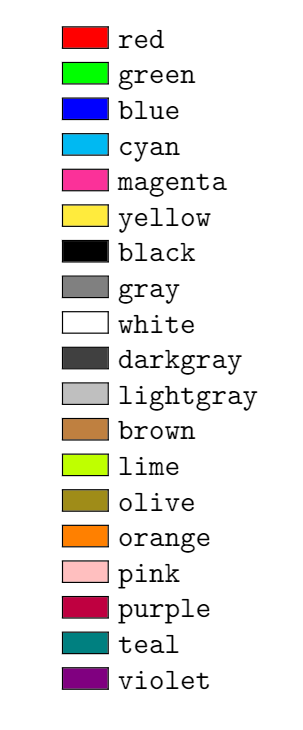
\includegraphics[width=0.7\linewidth]{files/05_xcolorList-efd7422e4e3a9a73a3353c9cd5d66686.png}
\caption[]{Osnovne barve, ki jih določa paket \texttt{xcolor}.}
\label{tbl:basecolors}
\end{figure}

Seznam določenih barv lahko razširimo z uporabo možnosti, ki jih ponuja paket \texttt{xcolor}. Npr z možnostjo \texttt{dvipsnames} lahko uporabimo dodatne barve prikazane v Figure~\ref{tbl:dvipsnames}.

\begin{figure}[!htbp]
\centering
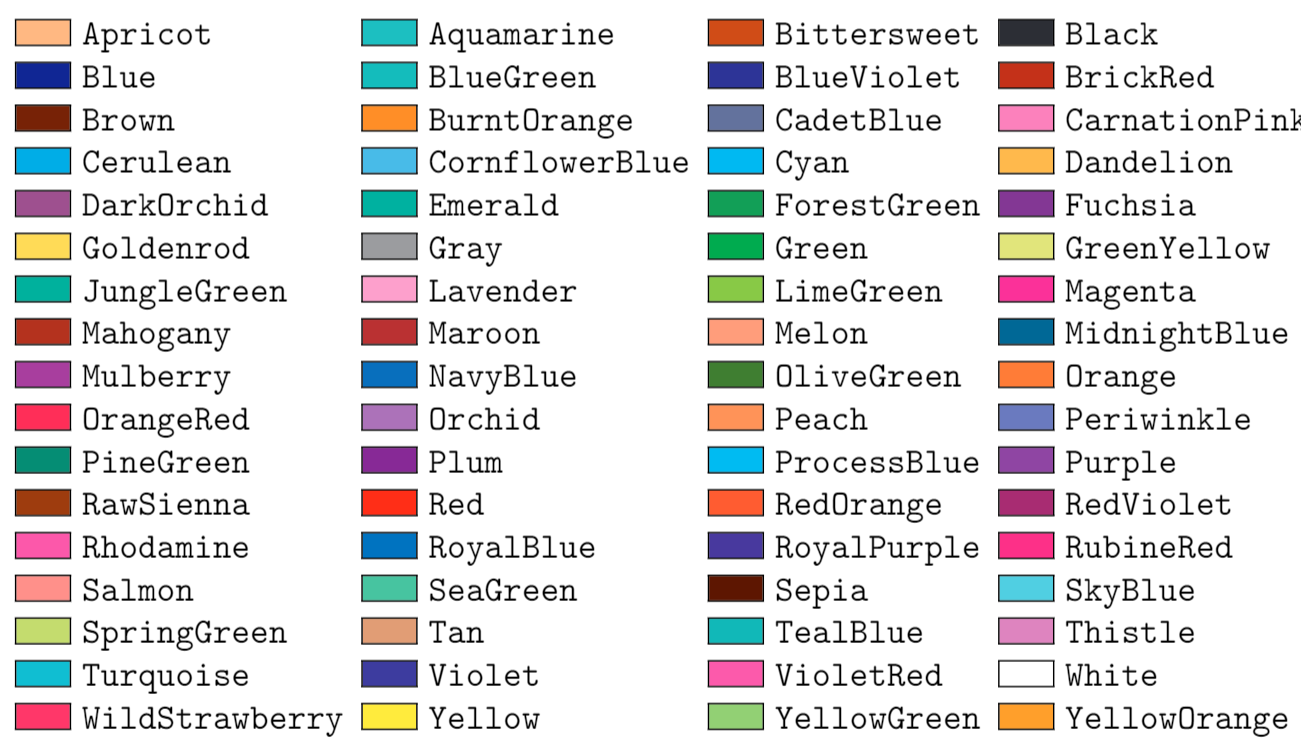
\includegraphics[width=0.7\linewidth]{files/05_xcolorDvipsnames-b995f7f9faffa70345f1476c434c77bc.png}
\caption[]{Dodatne barve, ki jih določa paket \texttt{xcolor} z možnostjo \texttt{dvipsnames}.}
\label{tbl:dvipsnames}
\end{figure}

Druge možnosti so \texttt{svgnames}, \texttt{x11names}. Možnost \texttt{svgnames} določa 151 barv, ki so definirane v SVG standardu, medtem ko možnost \texttt{x11names} določa 317 barv, ki so bile prvotno definirane za X11 Window System. Celoten seznam barv je na voljo v dokumentaciji paketa \href{https://ctan.org/pkg/xcolor?lang=en}{\texttt{xcolor}}.

Drugi način pridobivanja novih barv je z mešanjem dveh ali več barv. Sintaksa za mešanje dveh barv je naslednja:

\begin{verbatim}
<barva1>!<odstotno>!<barva2>
\end{verbatim}

Rezultat je barva, ki je sestavljena iz \texttt{\textless odstotno\textgreater } odstotkov \texttt{\textless barva1\textgreater } in \texttt{(100 - \textless odstotno\textgreater )} odstotkov \texttt{\textless barva2\textgreater }. Na primer, \texttt{red!40!blue} ustvari vijolično barvo, ki je mešanica 40\% rdeče in 60\% modre.

Mešanje lahko vključuje tudi več kot dve barvi. V tem primeru, mešanje je izvedeno zaporedno. Na primer, \texttt{red!50!green!30!blue} najprej zmeša 50\% rdeče in 50\% zelene, nato pa rezultat zmeša z 70\% modre in 30\% prej dobljene barve.

Včasih moramo biti natančnejši pri barvah, ki jih uporabljamo. Za to lahko uporabimo izbirni argument \texttt{model}. Najlažje ga razumemo prek modela \texttt{Gray}. V tem modelu določimo odtenek sive barve z vrednostjo med \texttt{0} in \texttt{15}, kjer \texttt{0} predstavlja črno in \texttt{15} belo.

Podobno lahko uporabimo model \texttt{grey}, kjer vrednosti segajo od \texttt{0} do \texttt{1}, pri čemer \texttt{0} predstavlja črno in \texttt{1} belo.

V Table~\ref{tbl:color-models} so prikazani nekateri barvni modeli, ki jih podpira paket \texttt{xcolor}.

% \begin{table}
% \centering
% \caption[]{Najpogostejši modeli barv v paketu \texttt{xcolor}}
% \label{tbl:color-models}
% \begin{tabular}{p{\dimexpr \linewidth-2\tabcolsep}}
% \toprule
% Model & Osnovne barve/komponente & Razpon parametrov & Primer \\
% \hline
% \texttt{rgb} & Rdeča, zelena, modra & $[0,1]^3$ & \texttt{{\textbackslash}textcolor[rgb]\{1,0,0\}\{Rdeča\}} \\
% \texttt{RGB} & Rdeča, zelena, modra & $\{0, \dots, 255\}^3$ & \texttt{{\textbackslash}textcolor[RGB]\{255,0,0\}\{Rdeča\}} \\
% \texttt{HTML} & Rdeča, zelena, modra & Šestnajstiški zapis & \texttt{{\textbackslash}textcolor[HTML]\{FF0000\}\{Rdeča\}} \\
% \texttt{cmy} & Cijan, magenta, rumena & $[0,1]^3$ & \texttt{{\textbackslash}textcolor[cmy]\{0,1,1\}\{Rdeča\}} \\
% \texttt{cmyk} & Cijan, magenta, rumena, črna & $[0,1]^4$ & \texttt{{\textbackslash}textcolor[cmyk]\{0,1,1,0\}\{Rdeča\}} \\
% \texttt{Gray} & Odtenek sive & $\{0, \dots, 15\}$ & \texttt{{\textbackslash}textcolor[Gray]\{0\}\{Črna\}} \\
% \texttt{gray} & Odtenek sive & $[0,1]$ & \texttt{{\textbackslash}textcolor[gray]\{0\}\{Črna\}} \\
% \texttt{wave} - Valovna dolžina (nm) - $[380,780]$ - \texttt{{\textbackslash}textcolor[wave]\{700\}\{Rdeča\}} \\
% \bottomrule
% \end{tabular}
% \end{table}

\begin{framed}
\textbf{Opozorilo!}\\
Pri mešanju barv v različnih modelih lahko dobimo nepričakovane rezultate. Na primer, da izrazi \texttt{\textless barva1\textgreater !25!\textless barva2\textgreater } in \texttt{\textless barva2\textgreater !75!\textless barva1\textgreater } ne dajeta vedno iste barve, če sta \texttt{\textless barva1\textgreater } in \texttt{\textless barva2\textgreater } definirani v različnih barvnih modelih.
Zato je priporočljivo, da pri mešanju barv vedno uporabljamo barve iz istega modela.
Alternativno v poglavje 6 dokumentacije paketa \href{https://ctan.org/pkg/xcolor?lang=en}{\texttt{xcolor}} najdemo več informacij o spremenjenju med barvnimi modeli.
\end{framed}

Z uporabo ukaza \texttt{{\textbackslash}definecolor\{\textless ime\_barve\textgreater \}\{\textless model\textgreater \}\{\textless parametri\textgreater \}} (v preambuli) lahko definiramo svoje barve. Na primer, z ukazom \texttt{{\textbackslash}definecolor\{ULrdeca\}\{RGB\}\{226,25,30\}} definiramo barvo z imenom \texttt{ULrdeca}, ki je rdeča barva Univerze v Ljubljani.

Doslej smo obravnavali ukaze za barvanje besedila. Možno je tudi spremeniti barbo ozadja strani z ukazom

\begin{verbatim}
\pagecolor[<model>]{<barva>}.
\end{verbatim}

Ta ukaz je različica \textit{switch}, to pomeni da spremeni barvo celotne strani od mesta, kjer je uporabljen, naprej. Če želimo vrniti nazaj privzeto barvo ozadja (prozoren), uporabimo ukaz \texttt{{\textbackslash}nopagecolor}.

V izrazu za barvo lahko uporabimo znak \texttt{-} (minus), da dobimo nasprotno barvo. Na primer, \texttt{-white} predstavlja črno barvo.

Če želimo spremeniti barvo samo določenega območja besedila, lahko uporabimo ukaz \texttt{{\textbackslash}colorbox[\textless model\textgreater ]\{\textless barva\textgreater \}\{\textless besedilo\textgreater \}}.
Ta ukaz obdaja besedilo z ozadjem določene barve.
Ukaz \texttt{{\textbackslash}fcolorbox[\textless model\textgreater ]\{\textless barva\_okvirja\textgreater \}\{\textless barva\_ozadja\textgreater \}\{\textless besedilo\textgreater \}} obdaja besedilo z okvirjem določene barve in ozadjem določene barve.

\subsubsection{Ukazi in okolja po meri.}

LaTeX omogoča ustvarjanje lastnih ukazov in okolij, kar lahko olajša pisanje ponavljajočih se struktur v dokumentu.
Klasični način za definiranje novega ukaza je z uporabo ukaza \texttt{{\textbackslash}newcommand\{\textless ime\_ukaza\textgreater \}[\textless število\_argumentov\textgreater ]\{\textless definicija\textgreater \}} in novega okolja z uporabo ukaza \texttt{{\textbackslash}newenvironment\{\textless ime\_okolja\textgreater \}[\textless število\_argumentov\textgreater ]\{\textless začetek\_definicije\textgreater \}\{\textless konec\_definicije\textgreater \}}.
Čeprav ti ukazi delujejo povsem normalno za osnovne definicije novih ukazov in okolij, bodo postopoma postali zastareli.
Tega pristopa tukaj ne bomo obravnavali, vendar če bralca zanima, priporočamo branje Overleafovih navodil za \href{https://www.overleaf.com/learn/latex/Commands}{nove ukaze}\{target=\_blank\} in \href{https://www.overleaf.com/learn/latex/Environments}{nova okolja}\{target=\_blank\} (v angleščini).

Sodobnejši in bolj zmogljiv način za definiranje novih ukazov in okolij je z uporabo ukaza \texttt{{\textbackslash}NewDocumentCommand} in \texttt{{\textbackslash}NewDocumentEnvironment}.
Ta pristop omogoča bolj fleksibilno določanje argumentov in podpira različne vrste argumentov, kot so obvezni, neobvezni, in več vrst argumentov.

Ukaz \texttt{{\textbackslash}NewDocumentCommand} ima naslednjo sintakso:

\begin{verbatim}
\NewDocumentCommand{<ime_ukaza>}{<vrsta_argumentov>}{<definicija>}
\end{verbatim}

\begin{itemize}
\item \texttt{\textless ime\_ukaza\textgreater }: Ime novega ukaza, ki ga želimo definirati (vključno z \texttt{{\textbackslash}}).
\item \texttt{\textless vrsta\_argumentov\textgreater }: Niz, ki določa vrste argumentov, ki jih ukaz sprejema. To bomo počasi obravnavali v nadaljevanju.
\item \texttt{\textless definicija\textgreater }: Telo ukaza, kjer lahko uporabimo argumente znotraj ukaza.
\end{itemize}

Najlažje ukaz, da lahko definiramo je brez argumentov, to pomeni z praznim nizom za \texttt{\textless vrsta\_argumentov\textgreater }.

Ta način je zelo uporaben, ko obstajajo del besedila ali strukture, ki jih pogosto uporabljamo v dokumentu.
Seveda, če se kdajkoli odločimo spremeniti to besedilo ali strukturo, moramo to storiti samo na enem mestu: v definiciji ukaza.

Pogosta uporaba novih ukazov je pri definiciji matematičnih izrazov, ki jih pogosto uporabljamo. Kot smo videli v prejšnjih poglavjih, nekatere vir (npr. \href{https://www.sist.si/velicine-in-enote-2-del-matematika-sist-en-iso-80000-220196-prevod-v-slovenscino.html}{Standard ISO 80000-2}) priporočajo, da se za matematične konstante in posebne funkcije uporablja rimska pisava (upravičeno).
Seveda, ni smiselno vsakič pisati \texttt{{\textbackslash}mathrm\{{\textbackslash}pi\}} za konstantno $\mathrm{pi}$ ali \texttt{{\textbackslash}mathrm\{e\}} za Eulerjevo število.
Namesto tega lahko definiramo nove ukaze za te konstante:

\begin{framed}
\textbf{Nasvet}\\
Ko definiramo nove ukaze, ki se bodo uporabljali v matematičnem načinu, je priporočljivo, da ne vključimo nobenega simbola, ki označuje matematični način.
Na primer, pri definiciji ukaza za konstantno $\pi$, je bolje definirati ukaz \texttt{{\textbackslash}kpi} kot \texttt{{\textbackslash}mathrm\{{\textbackslash}pi\}} namesto \texttt{\${\textbackslash}mathrm\{{\textbackslash}pi\}\$}.
\end{framed}

Če želimo definirati nov ukaz, ki sprejema argumente, moramo določiti vrsto in število argumentov v nizu \texttt{\textless vrsta\_argumentov\textgreater }.
Nekateri najpogostejši tipi argumentov so prikazani v Table~\ref{tbl:arg-types}.

\begin{table}
\centering
\caption[]{Najpogostejši tipi argumentov v \texttt{{\textbackslash}NewDocumentCommand}}
\label{tbl:arg-types}
\begin{tabular}{p{\dimexpr 0.500\linewidth-2\tabcolsep}p{\dimexpr 0.500\linewidth-2\tabcolsep}}
\toprule
Tip argumenta & Opis \\
\hline
\texttt{m} & Obvezni argument, ki lahko vsebuje več vrstic. \\
\texttt{O\{\textless privzeta\_vrednost\textgreater \}} & Neobvezni argument, ki lahko vsebuje več vrstic. Če ni podan, ima privzeto vrednost \texttt{\textless privzeta\_vrednost\textgreater }. \\
\texttt{o} & Neobvezni argument. Če ni podan, natisne posebni niz \texttt{-NoValue-}. Običajno v definicij uporaba pogojev za preverjanje, ali je bil argument podan kot je ukaz \texttt{{\textbackslash}IfNoValueTF}. \\
\texttt{D\textless levo\textgreater \textless desno\textgreater \{\textless privzeta\_vrednost\textgreater \}} & Neobvezni argument, ki je obdan z \texttt{\textless levo\textgreater } in \texttt{\textless desno\textgreater }. Če ni podan, ima privzeto vrednost \texttt{\textless privzeta\_vrednost\textgreater }. Običajno se uporablja znak \texttt{\textless } in \texttt{\textgreater }, za \texttt{\textless levo\textgreater } in \texttt{\textless desno\textgreater }. Deluje kot \texttt{o}, vendar s posebnimi ločevalniki. \\
\texttt{d\textless levo\textgreater \textless desno\textgreater } & Podobno kot \texttt{D}, vendar brez privzete vrednosti. Deluje kot \texttt{o}, vendar s posebnimi ločevalniki. \\
\texttt{s} & Preklopni argument (switch). Če je prisoten, je vrednost \texttt{{\textbackslash}BooleanTrue}, sicer \texttt{{\textbackslash}BooleanFalse}. Uporabno, ko definiramo ukaze `z zvezdico' ali `brez zvezdice'. \\
\bottomrule
\end{tabular}
\end{table}

Najlažje tip argumenta je \texttt{m}, ki predstavlja obvezni argument. Na primer, lahko definiramo ukaz za barvanje besedila z določenim in barvo. Pri definiciji ukazo, uporabljamo znak \texttt{\#1} za sklicevanje na prvi argument.

Seveda, lahko definiramo ukaze z več argumenti. Dovolj je da dodamo več tipov argumentov v niz \texttt{\textless vrsta\_argumentov\textgreater } in uporabimo \texttt{\#2}, \texttt{\#3}, ... za sklicevanje na druge argumente.

Če želimo definirati ukaz z neobveznimi argumenti, lahko uporabimo tip \texttt{O\{\textless privzeta\_vrednost\textgreater \}}. Ne pozabite, da neobvezni argumenti damo znotraj oklepaj \texttt{[]} pri klicu ukaza.

\begin{verbatim}
Lahko seveda kombiniramo različne tipe argumentov. Na primer, lahko definiramo ukaz z enim obveznim in enim neobveznim argumentom:

::::{grid} 2 2 2 2

:::{card} LaTeX

```latex
V preambuli:
\NewDocumentCommand{\Zap}{O{n}m}
{#2_{1}, \dots, #2_{#1}}
% V telesu dokumenta:
Nekatere zaporedje imajo veliko elementov:
$\Zap[1000]{a}$,
za večino pa sploh ne vemo,
koliko jih je:
$\Zap{b}$.
```

:::

:::{card} PDF

```{figure} ./img/05_eg -ArgsMO -1.png
:label: fig:eg -ArgsMO -1
```

:::
\end{verbatim}

Upoštevajte, da je vrstni red argumentov pomemben. Če je ukaz \texttt{{\textbackslash}ukaz} definiran z vrstnim redom argumentov \texttt{O\{\}m}, ga moramo klicati z obveznim argumentom najprej, nato pa neobveznim argumentom (če ga želimo podati), to pomeni \texttt{{\textbackslash}ukaz[\textless neobvezni\textgreater ]\{\textless obvezni\textgreater \}} je pravilen klic, medtem ko \texttt{{\textbackslash}ukaz\{\textless obvezni\textgreater \}[\textless neobvezni\textgreater ]} ni pravilen klic.
Dobra praksa je, da najprej definiramo vse neobvezne argumente, nato pa obvezne argumente.

Včasih želimo da ukaz deluje drugače, če je neobvezni argument podan ali ne. V tem primeru lahko uporabimo tip argumenta \texttt{o} in ukaz \texttt{{\textbackslash}IfValueTF} za preverjanje, ali je bil argument podan.

Namesto ukaza \texttt{{\textbackslash}IfValueTF}, lahko uporabimo tudi ukaz \texttt{{\textbackslash}IfValueT}, če želimo izvesti dejanje samo, če je bil argument podan, ali ukaz \texttt{{\textbackslash}IfValueF}, če želimo izvesti dejanje samo, če argument ni bil podan. Lahko tudi uporabimo ukaze \texttt{{\textbackslash}IfNoValueTF}, \texttt{{\textbackslash}IfNoValueT}, in \texttt{{\textbackslash}IfNoValueF}, ki delujejo nasprotno.

Ko želimo da ukaz sprejme neobvezni argument z določenimi ločevalniki, lahko uporabimo tip argumenta \texttt{D\textless levo\textgreater \textless desno\textgreater \{\textless privzeta\_vrednost\textgreater \}}.
Običajno se uporabljata znaka \texttt{\textless } in \texttt{\textgreater } kot ločevalnika.

Če namesto \texttt{D\textless levo\textgreater \textless desno\textgreater \{\textless privzeta\_vrednost\textgreater \}} uporabimo \texttt{d\textless levo\textgreater \textless desno\textgreater }, dobimo podoben učinek, vendar brez privzete vrednosti (točno tako, kot ko uporabljamo \texttt{o}). V tem primeru moramo vedno preveriti, ali je bil argument podan z uporabo ukaza \texttt{{\textbackslash}IfValueTF} in podobnih.

Nazadnje, lahko tudi uporabljamo znak \texttt{s} za niz \texttt{\textless vrsta\_argumentov\textgreater }, da definiramo preklopni argument oz. različica ukaz \textit{z zvezdico}. Pri definiciji ukaza, lahko uporabimo ukaz \texttt{{\textbackslash}IfBooleanTF}, da preverimo, ali je bil preklopni argument podan.

Lahko tudi definiramo nova okolja z uporabo ukaza \texttt{{\textbackslash}NewDocumentEnvironment}, ki ima podobno sintakso kot \texttt{{\textbackslash}NewDocumentCommand}.

\begin{verbatim}
\NewDocumentEnvironment{<ime_okolja>}{<vrsta_argumentov>}
{<začetek_definicije>}
{<konec_definicije>}
\end{verbatim}

\begin{itemize}
\item \texttt{\textless ime\_okolja\textgreater }: Ime novega okolja, ki ga želimo definirati.
\item \texttt{\textless vrsta\_argumentov\textgreater }: Niz, ki določa vrste argumentov, ki jih okolje sprejema. To deluje skoraj enako kot pri ukazu \texttt{{\textbackslash}NewDocumentCommand}.
\item \texttt{\textless začetek\_definicije\textgreater }: Koda za začetek okolja, kjer lahko uporabimo argumente znotraj okolja.
\item \texttt{\textless konec\_definicije\textgreater }: Koda za konec okolja.
\end{itemize}

Naslednji primeri naj bi pojasnili uporabo tega ukaza.

\begin{example}\label{eg_okolja_kralj-1}\end{example}Lahko tudi definiramo okolja z argumenti. Na primer, lahko definiramo okolje \texttt{kraljIme}, ki sprejme en obvezni argument za ime kralja.

\begin{example}\label{eg_okolja_kralj-2}\end{example}Tukaj imamo problem, ker želimo imeti različne naslove in zaključke za kralja in kraljico. To lahko rešimo z uporabo preklopnega argumenta \texttt{s}.
Moramo v definiciji okolja uporabiti ukaz \texttt{{\textbackslash}IfBooleanTF}, da preverimo, ali je bil preklopni argument podan; to lahko storimo v obeh delih definicije okolja.

Pazite, za razliko od nekaterih drugih LaTeX okoljih (npr. \texttt{align}), ko uporabljamo okolje z zvezdico, zvezdica gre zunaj oklepajev imenja okolja, t.j. \texttt{{\textbackslash}begin\{kralij\}*\{Ime\}} namesto \texttt{{\textbackslash}begin\{kralij*\}\{Ime\}}. Zvezdica ni potrebna na koncu okolja, t.j. \texttt{{\textbackslash}end\{kralij\}} je pravilen klic tudi za okolje z zvezdico.

\begin{example}\label{eg_kralji}\end{example}\subsubsection{Vaje}\label{05_latexRazno_vaje}

\begin{itemize}
\item Exercise~\ref{ex_input_include}: Vaje o ukazih \texttt{{\textbackslash}input\{\}} in \texttt{{\textbackslash}include\{\}}.
\item Exercise~\ref{ex-gradient}: Vaja o mešanju barv.
\item Exercise~\ref{ex_ukazi}: Vaje o definiciji novih ukazov z \texttt{{\textbackslash}NewDocumentCommand}.
\end{itemize}

\subsection{Beamer: Prestavitve v LaTeXu}

% https://www.overleaf.com/learn/latex/Beamer_Presentations%3A_A_Tutorial_for_Beginners_(Part_1)%E2%80%94Getting_Started

Beamer je LaTeX razširitev za izdelavo drsnic (``slajdov'').
Za izdelavo predstavitve z Beamerjem uporabimo razred \texttt{beamer} namesto \texttt{article}.
Nato uporabimo okolja \texttt{frame} za vsak posamezen diapozitiv.

\begin{framed}
\textbf{Glej tudi: Beamer uporabniški vodič.}\\
V tem poglaviu bomo predstavili osnovne koncepte in ukaze za ustvarjanje predstavitev z Beamerjem.
Za podrobnejše informacije in napredne funkcije si oglejte uradno \href{https://tug.ctan.org/macros/latex/contrib/beamer/doc/beameruserguide.pdf}{Beamer user guide}.
\end{framed}

\begin{framed}
\textbf{Opozorilo}\\
Razred \texttt{beamer} uporaba paket \texttt{babel} za jezike malo drugače kot običajni razredi dokumentov (kot so \texttt{article} ali \texttt{report}).
V tem razredu je priporočljivo, da je jezik dokumenta določen kot možnost razreda dokumenta (npr. \texttt{{\textbackslash}documentclass[slovene]\{beamer\}}) in da se paket \texttt{babel} naloži brez možnosti jezika (npr. \texttt{{\textbackslash}usepackage\{babel\}}).
\end{framed}

Ukaz \texttt{{\textbackslash}frametitle\{\}} določi naslov drsnice. Lahko tudi uporabimo ukaz \texttt{framesubtitle\{\}} za podnaslov drsnice.
Krajša možnost je, da naslov oz. podnaslov drsnice podamo kot možnost okolja \texttt{frame}; Example~\ref{eg_beamer_1}.

\begin{example}\label{eg_beamer_1}\end{example}\subsubsection{Pomembne drsnice}

Podobno kot pri člankih lahko tudi pri Beamer predstavitvah ustvarimo naslovni diapozitiv z uporabo ukazov \texttt{{\textbackslash}title\{\}}, \texttt{{\textbackslash}author\{\}} in \texttt{{\textbackslash}date\{\}} v preambuli dokumenta.

Zdaj ukaz \texttt{{\textbackslash}maketitle} v telesu dokumenta ustvari naslovni diapozitiv. Ukaz \texttt{{\textbackslash}maketitle} je enakomerno kot

\begin{verbatim}
\begin{frame}
\titlepage
\end{frame}
\end{verbatim}

Običajno ukaz \texttt{{\textbackslash}date} nastavimo na ime konference ali dogodek, kjer bo predstavitev prikazana.
V razreed beamer lahko tudi uporabljamo ukaze \texttt{{\textbackslash}institute\{\}}, \texttt{{\textbackslash}subtitle\{\}} in \texttt{{\textbackslash}titlegraphic\{\}} za dodajanje dodatnih informacij na naslovno drsnico; poglejte Example~\ref{eg_beamer-title-1}.

\begin{example}\label{eg_beamer-title-1}\end{example}Nekatere teme Bemerja (glej Teme~in~barvne~sheme) dodajo informacije o avtorju in datumu na vsako drsnico.
Če je vsebina teh polj predolga, ne bo dovolj prostora; v tem primeru lahko dodamo neobvezni kratek argument v ukaze (npr. \texttt{{\textbackslash}author[\textless kratek\textgreater ]\{\textless dolg\textgreater \}}), ki se bo prikazal v glavi ali nogi drsnice, poglejte Example~\ref{eg_beamer-title-2}.

\begin{example}\label{eg_beamer-title-2}\end{example}Ukaz \texttt{{\textbackslash}titlegraphic\{\}} doda sliko na naslovno drsnico.
Če želimo dodati logotip na vse drsnice, lahko uporabimo ukaz \texttt{{\textbackslash}logo\{\}} v preambuli dokumenta, poglejte Example~\ref{eg_beamer-logo}.
Upoštevajte, da je pozicija logotipa odvisna od uporabljene teme. Poleg tega, nekatere teme ne podpirajo logotipov/grafik na naslovni drsnici.

\begin{example}\label{eg_beamer-logo}\end{example}V razredu beamer lahko tudi uporabimo ukaze za \textit{logične strukture} kot so \texttt{{\textbackslash}section\{\}} in \texttt{{\textbackslash}subsection\{\}} za organizacijo predstavitve.
Ti ukazi ne ustvarijo drsnic, vendar jih lahko uporabimo za generiranje kazala vsebine.
To lahko storimo z uporabo ukaza \texttt{{\textbackslash}tableofcontents} v okolju \texttt{frame}, poglejte Example~\ref{eg_beamer-toc-1}.
Upoštevajte, da razdelek \texttt{Literatura} ni v kazalo vključen, ker je definiran z ukazom \texttt{{\textbackslash}section*\{\}}.

\begin{example}\label{eg_beamer-toc-1}\end{example}Če želimo kazalo prikazati postopoma, lahko k ukazom \texttt{{\textbackslash}tableofcontents} dodamo možnost \texttt{pausesections}. Poglejte Example~\ref{eg_beamer-toc-2}.

\begin{example}\label{eg_beamer-toc-2}\end{example}Ukaze kot \texttt{{\textbackslash}section} ne ustvarijo drsnic, vendar lahko z ukazom \texttt{{\textbackslash}sectionpage} znotraj okolja \texttt{frame} ustvarimo drsnico, ki prikazuje naslov razdelka.

%  Na žalost, ukaz `\sectionpage` ni dela skupaj z paketom `babel`.

Druga možnost je ponatis kazala na začetku vsakega poglavja, da bralce spomnimo, kje smo.
To lahko storimo z uporabo ukazov \texttt{{\textbackslash}AtBeginSection[]} in \texttt{{\textbackslash}tableofcontents[currentsection]} poglejte Example~\ref{eg_beamer-toc-3}. Če želimo, da se v kazalu prikažejo samo razdelek (in ne podrazdelek), dodamo ukaz {\textbackslash}tableofcontents opcijo \texttt{hidesubsections}.

\begin{example}\label{eg_beamer-toc-3}\end{example}Poleg ukazov \texttt{{\textbackslash}section} in \texttt{{\textbackslash}subsection}, Beamer podpira tudi ukaz \texttt{{\textbackslash}part\{\}} za večje logične enote.
Vsak del prestavitve (definiran z \texttt{{\textbackslash}part\{\}}) lahko začne z drsnico, ki prikazuje naslov dela z uporabo ukaza \texttt{{\textbackslash}partpage} v okolju \texttt{frame}. Poleg tega, ima vsak del lahko svoje kazalo vsebine; poglejte Example~\ref{eg_beamer-parts}.

\begin{example}\label{eg_beamer-parts}\end{example}\subsubsection{Specifikacije prekrivanja}\label{beamer_prekrivanje}

Izhodna datoteka Beamer je običajno v formatu \texttt{PDF} kar je v principu statična datoteka. Beamer pa omogoča ustvarjanje dinamičnih učinkov z uporabo \textit{specifikacij prekrivanja} (ang. \textit{overlay specifications}).

Prestavitve Beamer sestoji iz serie drsnic, vsaka drsnica pa je lahko razdeljena na več slojev oz. stran (ang. \textit{slides}). V izhodni \texttt{PDF} datoteki vsak sloj ustreza eni strani. Specfikacije prekrivanja so ukazi, ki določajo, kateri deli vsebine so prikazani na določenem sloju.

Najlažji način za uporabo specifikacij prekrivanja je z uporabo ukaza \texttt{{\textbackslash}pause}, ki ustvari prekinitev na trenutni točki v drsnici.
Če dodamo ukaz \texttt{{\textbackslash}pause} v okolje \texttt{frame}, prvi sloj drsnice prikaže vsebino do prva uporaba ukaza \texttt{{\textbackslash}pause}, drugi sloj prikaže vsebino do druge uporabe ukaza \texttt{{\textbackslash}pause} in tako naprej. Poglejte Example~\ref{eg_beamer-pause}.

\begin{example}\label{eg_beamer-pause}\end{example}Ukaz \texttt{{\textbackslash}pause} je enostaven za uporabo, vendar ponuja omejene možnosti prilagajanja. Za bolj natančno kontrolo nad tem, kdaj se posamezni deli vsebine prikažejo, lahko uporabimo \textit{specifikacije prekrivanja} znotraj ukazov kot so \texttt{{\textbackslash}textbf}, \texttt{{\textbackslash}textit}, \texttt{{\textbackslash}textcolor} in druge (poglejte Table~\ref{tab-prekrivanje-ukaze}).

Sintaksa za specifikacije prekrivanja je naslednja:

\begin{verbatim}
\ukaz<spec_prek>{<besedilo>}
\end{verbatim}

Kjer \texttt{{\textbackslash}ukaz} predstavlja ukaz, ki ga želimo nadzorovati (npr. \texttt{{\textbackslash}textbf}), \texttt{spec\_prek} pa določa, na katerih slojih bo ukaz uporabljen. Na primer, \texttt{{\textbackslash}textbf\textless 2\textgreater \{\textless besedilo\textgreater \}} bo prikazalo \texttt{\textless besedilo\textgreater } krepko le na drugem sloju drsnice (ostali sloji bodo prikazali \texttt{\textless besedilo\textgreater } v običajnem slogu); poglejte Example~\ref{eg_beamer-overlay-1}.

\begin{example}\label{eg_beamer-overlay-1}\end{example}Nekatere ukaze, kot so \texttt{{\textbackslash}item} v okolju \texttt{itemize} in \texttt{enumerate}, imajo vgrajeno podporo za specifikacije prekrivanja; poglejte Example~\ref{eg_beamer-overlay-2}.

\begin{example}\label{eg_beamer-overlay-2}\end{example}Ukaz {\textbackslash}includegraphics podpira tudi specifikacije prekrivanja, kar omogoča prikazovanje različnih slik na različnih slojih drsnice. To je uporabno za simulacijo animacij z zaporednim prikazovanjem slik;
poglejte Example~\ref{eg_beamer-overlay-3}.

\begin{example}\label{eg_beamer-overlay-3}\end{example}\href{/stick-3a960172ac01f90300a20c6f2227b668.zip}{\texttt{stick.zip}} vsebuje slike, uporabljene v zgornjem primeru.

Naslednje tri ukaze delujejo zelo podobno. Prikazujejo \texttt{\textless besedilo\textgreater } v skladu z \texttt{\textless spec\_prek\textgreater }. Razlika med njimi je v tem, kako se obnašajo, ko besedilo ni prikazano.

\begin{itemize}
\item \texttt{{\textbackslash}only\textless spec\_prek\textgreater \{\textless besedilo\textgreater \}}: Prikaže \texttt{\textless besedilo\textgreater } samo na slojih, določenih z \texttt{\textless spec\_prek\textgreater }. Na drugih slojih \texttt{\textless besedilo\textgreater } ni prisotno (ne zavzame prostora).
\item \texttt{{\textbackslash}visible\textless spec\_prek\textgreater \{\textless besedilo\textgreater \}}: Prikaže \texttt{\textless besedilo\textgreater } na slojih, določenih z \texttt{\textless spec\_prek\textgreater }, in na drugih slojih ohrani prostor, ki ga \texttt{\textless besedilo\textgreater } zavzema (vendar je \textbf{nevidno}).
\item \texttt{{\textbackslash}uncover\textless spec\_prek\textgreater \{\textless besedilo\textgreater \}}: Prikaže \texttt{\textless besedilo\textgreater } na slojih, določenih z \texttt{\textless spec\_prek\textgreater }, in na drugih slojih ohrani prostor, ki ga \texttt{\textless besedilo\textgreater } zavzema (vendar je \textbf{prozoren}).
\end{itemize}

Razlika med \texttt{{\textbackslash}visible} in \texttt{{\textbackslash}uncover} je odvisno od uporabe \textit{prosojnosti} (ang. \textit{transparency}). To se nadzoruje z ukazom \texttt{{\textbackslash}setbeamercovered\{\textless možnost\textgreater \}} v preambuli dokumenta. Možnosti vključujejo:

\begin{itemize}
\item \texttt{invisible}: Besedilo je popolnoma nevidno (privzeta možnost).
\item \texttt{transparent=\textless neprosojnost\textgreater }: Besedilo je prikazano z določeno stopnjo prosojnosti: \texttt{\textless neprosojnost\textgreater } je vrednost med \texttt{0} (popolnoma prozorno) in \texttt{100} (popolnoma neprozorno); privzeta vrednost je \texttt{15}.
\item \texttt{dynamic}: Vse prekrite besede postanejo precej prosojne, vendar na dinamičen način. Daljši čas potreben za odkritje besedila, močnejša je prosojnost. Poglejte Example~\ref{eg_overlays-only-1}.
\end{itemize}

\begin{example}\label{eg_overlays-only-1}\end{example}Obstajajo še drugi ukazi za specifikacije prekrivanja, kot so:

\begin{itemize}
\item \texttt{{\textbackslash}invisible\textless spec\_prek\textgreater \{\textless besedilo\textgreater \}}: Točno nasprotje ukaza \texttt{{\textbackslash}visible}. Prikaže \texttt{\textless besedilo\textgreater } na slojih, določenih z \texttt{\textless spec\_prek\textgreater }, in na drugih slojih besedilo ni prisotno.
\item \texttt{{\textbackslash}alt\textless spec\_prek\textgreater \{\textless besedilo1\textgreater \}\{\textless besedilo2\textgreater \}}: Prikaže \texttt{\textless besedilo1\textgreater } na slojih določenih z \texttt{\textless spec\_prek\textgreater }, in \texttt{\textless besedilo2\textgreater } na ostalih slojih.
\item \texttt{{\textbackslash}temporal\textless spec\_prek\textgreater \{\textless besedilo1\textgreater \}\{\textless besedilo2\textgreater \}\{\textless besedilo3\textgreater \}}: Prikaže \texttt{\textless besedilo1\textgreater } pred prvi sloji določenimi z \texttt{\textless spec\_prek\textgreater }, \texttt{\textless besedilo2\textgreater } na slojih določenih z \texttt{\textless spec\_prek\textgreater }, in \texttt{\textless besedilo3\textgreater } po zadnji sloji določeni z \texttt{\textless spec\_prek\textgreater }.
\end{itemize}

V Example~\ref{eg_overlays-only-2} so prikazani ti ukazi v akciji.

\begin{example}\label{eg_overlays-only-2}\end{example}Nekatere okolje v Beamerju podpirajo specifikacije prekrivanja.
Sintaksa je običajno \texttt{{\textbackslash}begin\{okolja\}\textless spec\_prek\textgreater } in rezultat je, da se celotno okolje prikaže samo na slojih določenih z \texttt{\textless spec\_prek\textgreater }.

Vsak od ukazov \texttt{{\textbackslash}only}, \texttt{{\textbackslash}alt}, \texttt{{\textbackslash}visible}, \texttt{{\textbackslash}uncover} in \texttt{{\textbackslash}invisible} ima svojo različico okolja, in sicer, \texttt{onlyenv}, \texttt{altenv}, \texttt{visibleenv}, \texttt{uncoverenv} in \texttt{invisibleenv}.
Vsi razen \texttt{altenv} ima sintakso

\begin{verbatim}
\begin{okolja}<spec_prek>
  <vsebina>
\end{okolja}
\end{verbatim}

in delujejo podobno kot njihovi ukazni ekvivalenti.
Okolje \texttt{altenv} ima sintakso

\begin{verbatim}
\begin{altenv}<spec_prek>
{<begin_privzeto>}{<end_privzeto>}
{<begin_alternativno>}{<end_alternativno>}
  <vsebina>
\end{altenv}
\end{verbatim}

V določenih slojih določenih z \texttt{\textless spec\_prek\textgreater }, se \texttt{\textless vsebina\textgreater } obdana med \texttt{\textless begin\_privzeto\textgreater } in \texttt{\textless end\_privzeto\textgreater }, medtem ko se v ostalih slojih prikaže vsebina obdana z \texttt{\textless begin\_alternativno\textgreater } in \texttt{\textless begin\_alternativno\textgreater }.

Lahko uporabimo ukaze kot je \texttt{{\textbackslash}only} za dinamično spremeniti vsebino drsnice, npr.

\begin{verbatim}
\only<1>{Besedilo za prvi sloj.}
  \only<2>{Besedilo za drugi sloj, ki je lahko daljše. Če je besedilo daljše, se okvir prilagodi višini vsebine.}
  \only<3>{Tretji sloj ima spet krajše besedilo.}
\end{verbatim}

Težava pri tem pristopu je, da lahko pride do nadležnih razlik v višini
elementov, kar lahko povzroči, da se celoten okvir >>trese<< od sloja do sloja.

Za rešitev tega problema lahko uporabimo okolje \texttt{overlayarea}, ki ima naslednjo sintakso:

\begin{verbatim}
\begin{overlayarea}{<širina>}{<višina>}
  <vsebina>
\end{overlayarea}
\end{verbatim}

To okolje ustvari območje \texttt{\textless širina\textgreater } krat \texttt{\textless višina\textgreater }, v katerem se vsebina lahko dinamično spreminja brez vpliva na višino okvirja drsnice; poglejte Example~\ref{eg_overlayarea}.

\begin{example}\label{eg_overlayarea}\end{example}\subsubsection{Vsebina predstavitve}\label{beamer_vsebina}

\paragraph{Seznami}

Navadna okolja za sezname, kot so \texttt{itemize}, \texttt{enumerate} in \texttt{description}, so podprta v Beamerju.

Seveda lahko uporabimo tudi ukaz \texttt{{\textbackslash}pause} ali specifikacije prekrivanja kot prikazano v Example~\ref{eg_beamer-overlay-2} za postopno prikazovanje elementov seznama.
Druga možnost je uporaba speficikacije \texttt{[\textless +-\textgreater ]} v okolju seznama, kar samodejno prikaže vsak element na naslednjem sloju; poglejte Example~\ref{eg_beamer-lists-1}.

V tem primeru tudi pokažemo uporabo ukaza \texttt{{\textbackslash}vspace\{\textless višina\textgreater \}} za ustvarjanje navpičnega prostora med seznami in ukaza \texttt{{\textbackslash}vfill}, ki potisne vsebino navzdol do dna okvirja drsnice.

\begin{example}\label{eg_beamer-lists-1}\end{example}Če je seznam predolg, da bi ga lahko prikazali na eni drsnici. V tem primeru lahko uporabimo pristop, ki ga prikazuje Example~\ref{eg_beamer-lists-2}.

\begin{example}\label{eg_beamer-lists-2}\end{example}\paragraph{Stolpci}

Beamer omogoča ustvarjanje stolpcev z uporabo okolja \texttt{columns}. Vsak stolpec je definiran z okoljem \texttt{column}, ki ima naslednjo sintakso:

\begin{verbatim}
\begin{columns}
  \begin{column}<spec_prek>{<širina>}
    <vsebina stolpca 1>
  \end{column}
  \begin{column}<spec_prek>{<širina>}
    <vsebina stolpca 2>
  \end{column}
  ...
\end{columns}
\end{verbatim}

Kjer \texttt{\textless širina\textgreater } določa širino stolpca (lahko je absolutna vrednost, npr. \texttt{5cm}, ali relativna vrednost, npr. \texttt{0.5{\textbackslash}textwidth}), \texttt{\textless spec\_prek\textgreater } pa so opcijske specifikacije prekrivanja, ki določajo, na katerih slojih bo stolpec prikazan.
Poglejte Example~\ref{eg_beamer-columns-1}.

\begin{example}\label{eg_beamer-columns-1}\end{example}Ta pristop lahko uporabimo za ustvarjanje drsnic z besedilom na eni strani in sliko na drugi strani; poglejte Example~\ref{eg_beamer-columns-2}.

\begin{example}\label{eg_beamer-columns-2}\end{example}\paragraph{Tabele}

Na splošno večina ukazov, ki smo jih opisali
v poglavju \href{/latexosnovnaokolja}{Osnovna okolja} za ustvarjanje tabel v LaTeX-u deluje tudi v Beamerju, dokler naložimo ustrezne pakete (npr. \texttt{booktabs}, \texttt{array}, \texttt{multrow}).

Poleg tega lahko uporabimo specifikacije prekrivanja za postopno prikazovanje vrstic ali stolpcev v tabeli; poglejte Example~\ref{eg_beamer-tables-1}.

\begin{example}\label{eg_beamer-tables-1}\end{example}Če je tabela preširoka ali predolga za drsnico, lahko uporabimo okolje \texttt{resizebox} iz paketa \texttt{graphicx}. Sintaksa je \texttt{{\textbackslash}resizebox\{\textless širina\textgreater \}\{\textless višina\textgreater \}\{\textless vsebina\textgreater \}}, kjer lahko uporabimo \texttt{!} za samodejno prilagoditev višine ali širine glede na drugo dimenzijo.
Poglejte Example~\ref{eg_beamer-tables-2}.

\begin{example}\label{eg_beamer-tables-2}\end{example}\paragraph{Bloki}

Beamer ponuja okolje \texttt{block} za ustvarjanje poudarjenih vsebinskih blokov znotraj drsnic. Sintaksa je naslednja:

\begin{verbatim}
\begin{block}{<naslov bloka>}
  <vsebina bloka>
\end{block}
\end{verbatim}

Poleg tega Beamer ponuja posebne vrste blokov, kot so \texttt{exampleblock} in \texttt{alertblock}, ki imajo različne sloge za poudarjanje vsebine. Slog bloka je odvisen od izbrane teme Beamerja. Poglejte Example~\ref{eg_beamer-blocks-1}.

\begin{example}\label{eg_beamer-blocks-1}\end{example}Okolje za teoreme, kot so \texttt{theorem}, \texttt{lemma}, \texttt{definition}, \texttt{proof}, itd. so prav tako podprta v Beamerju in imajo slog, ki je podobno kot bloki. Poglejte Example~\ref{eg_beamer-blocks-2}.

\begin{example}\label{eg_beamer-blocks-2}\end{example}Lahko tudi definiramo svoje matematične bloke z uporabo ukaza \texttt{{\textbackslash}newtheorem} točno tako, kot v običajnem LaTeXu.

\subsubsection{Teme in barvne sheme}\label{beamer_teme}

Beamer ponuja različne teme in barvne sheme za prilagoditev videza predstavitve. Teme določajo splošno postavitev in slog drsnic, in barvno paleto.

Obstajajo štiri parametri za prilagoditev videza predstavitve v Beamerju:

\begin{itemize}
\item Tema barv (ang. \texttt{color theme}): Določa barvno shemo predstavitve.
\item Tema pisave (ang. \texttt{font theme}): Določa slog pisave.
\item Notranje teme (ang. \texttt{inner theme}): Določa slog notranjih elementov, kot so sezname, bloki, kazalo, itd.
\item Zunanje teme (ang. \texttt{outer theme}): Določa slog zunanjih elementov, kot so glave, noge, okvirji drsnic, itd.
\end{itemize}

Poleg teh štirih parametrov lahko izberemo tudi celotno temo, ki združuje vse te vidike v eno samo temo. Večinoma časa, je dovolj, da izberemo samo temo, saj bo ta samodejno nastavila ustrezne barvne sheme, pisave in notranje ter zunanje teme in če želimo, lahko dodatno prilagodimo posamezne parametre.

Teme se naložijo z ukazom \texttt{{\textbackslash}usetheme\{\textless ime\_teme\textgreater \}}, medtem ko se posamezni parametri naložijo z ukazi

\begin{itemize}
\item \texttt{{\textbackslash}usecolortheme\{\textless ime\_barvne\_sheme\textgreater \}}
\item \texttt{{\textbackslash}usefonttheme\{\textless ime\_pisave\textgreater \}}
\item \texttt{{\textbackslash}useinnertheme\{\textless ime\_notranje\_teme\textgreater \}}
\item \texttt{{\textbackslash}useoutertheme\{\textless ime\_zunanje\_teme\textgreater \}}
\end{itemize}

Število možnosti za te ukaze je ogromno in nemogoče je prikazati vse relevantne primere.
Lahko pa ponudimo zunanje vire za raziskovanje različnih tem.

\begin{itemize}
\item \href{https://hartwork.org/beamer-theme-matrix/}{Beamer Theme Matrix}: Interaktivno orodje za raziskovanje različnih kombinacij tem in barvnih shem v Beamerju.
\item \href{https://deic.uab.es/~iblanes/beamer\_gallery/index.html}{Beamer Theme Gallery}: Galerija različnih tem Beamer, tem pisave in tem barv.
\item \href{https://tug.ctan.org/macros/latex/contrib/beamer/doc/beameruserguide.pdf}{Beamer User Guide}: Del III vodiča za uporabnike Beamerja vsebuje podrobne informacije o temah in barvnih shemah.
\item \href{https://www.overleaf.com/gallery/tagged/beamer}{Overleaf beamer templates}: Sodobne teme Beamer na Overleafu.
\end{itemize}

\subsubsection{Vaje}\label{06_latexBeamer_vaje}

\section{GeoGebra}

\subsection{GeoGebra: Uvod}

\subsubsection{Kaj je Geogebra?}

\href{https://www.geogebra.org/}{Geogebra} je brezplačno dinamično matematično orodje, ki omogoča raziskovanje in vizualizacijo različnih matematičnih konceptov.

Trenuto, Geogebra je popoln paket za učenje in poučevanje matematike. Ponuja različne aplikacije, ki pokrivajo področja, kot so geometrija, algebra, statistika in kalkulus.
Vse te aplikacije je mogoče namestiti lokalno ali dostopati do njih prek spleta:

\begin{itemize}
\item \href{https://www.geogebra.org/scientific}{Scientific Calculator}: Za izračune z ulomki, statistiko in osnovnimi matematičnimi funkcijami.
\item \href{https://www.geogebra.org/graphing}{Graphing Calculator}: Za vizualizacijo enačb in funkcij z interaktivnimi grafikoni.
\item \href{https://www.geogebra.org/geometry}{Geometry}: Za dinamične geometrijske koncepte in konstrukcije v ravnini.
\item \href{https://www.geogebra.org/3d}{3D Calculator}: Za raziskovanje tridimenzionalnih oblik in površin.
\item \href{https://www.geogebra.org/cas}{CAS Calculator}: Za simbolne izračune in reševanje enačb.
\item \href{https://www.geogebra.org/calculator}{Calculator suit}: Kombinacija različnih orodij za širok spekter matematičnih nalog. Idealna za učence in študente.
\item \href{https://www.geogebra.org/classic}{Geogebra Classic}: Vse-v-enem aplikacija, ki združuje vse zgoraj omenjene funkcije. Idealna za avtorije učnih gradiv.
\end{itemize}

Različne možnosti, ki jih ponuja vsako od orodij, so navedene v Table~\ref{tab_geogebra-apps}.

\begin{table}
\centering
\caption[]{Primerjava različnih aplikacij Geogebra}
\label{tab_geogebra-apps}
\begin{tabular}{p{\dimexpr 0.125\linewidth-2\tabcolsep}p{\dimexpr 0.125\linewidth-2\tabcolsep}p{\dimexpr 0.125\linewidth-2\tabcolsep}p{\dimexpr 0.125\linewidth-2\tabcolsep}p{\dimexpr 0.125\linewidth-2\tabcolsep}p{\dimexpr 0.125\linewidth-2\tabcolsep}p{\dimexpr 0.125\linewidth-2\tabcolsep}p{\dimexpr 0.125\linewidth-2\tabcolsep}}
\toprule
aplikacije / funkcije & Scientific & Graphing & Geometry & 3D & CAS & Suit & Classic \\
\hline
Numerični izračuni & x & x & x & x & x & x & x \\
Funkcije & x & x & x & x & x & x & x \\
Operacije z ulomki & x & x & x & x & x & x & x \\
Grafično prikazovanje &  & x & x & x & x & x & x \\
Drsniki &  & x & x & x & x & x & x \\
Vektorji in matrike &  & x & x & x & x & x & x \\
Tabele &  & x &  &  & x & x & x \\
Geometrijske konstrukcije &  &  & x & x & x & x & x \\
3D prikazovanje &  &  &  & x &  & x & x \\
Verjetnost in statistika &  &  &  &  &  & x & x \\
Odvodi in integrali &  &  &  & x & x & x & x \\
Reševanje enačb &  &  &  & x & x & x & x \\
Simbolni izračuni &  &  &  & x & x & x & x \\
Spreadsheets &  &  &  &  &  &  & x \\
\bottomrule
\end{tabular}
\end{table}

Mi bomo v nadaljevanju uporabljali predvsem \href{https://www.geogebra.org/classic}{Geogebra Classic}, saj omogoča uporabo vseh orodij na enem mestu.

\subsubsection{Kako začnemo z Geogebro?}

Geogebra lahko uporabimo na dva načina: prek spletnega brskalnika ali z namestitvijo aplikacije na računalnik (ali telefon/tablet).

V vsakem primeru bomo uporabili račun Geogebra, ki nam omogoča shranjevanje naših delovnih zvezkov v oblak in dostop do njih od kjerkoli.

Zdaj imate dve možnosti za začetek uporabe Geogebre:

\begin{enumerate}
\item \textbf{Uporaba spletnega brskalnika}:

\begin{itemize}
\item Obiščite \href{https://www.geogebra.org/classic}{Geogebra Classic}.
\item Kliknite na gumn  
\includegraphics[width=0.0275\linewidth]{files/16px-Menu-button-ope-f5b0cc09aa629bb7475641338f148b1b.png}

 \textit{Menu} v zgornjem levem kotu.
\item Prijavite se s svojim računom z klikom na  
\includegraphics[width=0.0275\linewidth]{files/16px-Menu-signin-720b9ea9464a31ca1f9e7d8d070c2f8e.png}

 \textit{Sign in}.
\end{itemize}


\item \textbf{Namestitev aplikacije}:

\begin{itemize}
\item Prenesite aplikacijo Geogebra Classic za vaš operacijski sistem z \href{https://geogebra.github.io/docs/reference/en/GeoGebra\_Installation/\#\_geogebra\_classic\_6}{uradne strani za prenos}.
\item Namestite aplikacijo in jo odprite.
\item Prijavite se s svojim računom z klikom na gumb 
\includegraphics[width=0.0275\linewidth]{files/16px-Menu-button-ope-f5b0cc09aa629bb7475641338f148b1b.png}

 \textit{Menu}  v zgornjem levem kotu in nato na 
\includegraphics[width=0.0275\linewidth]{files/16px-Menu-signin-720b9ea9464a31ca1f9e7d8d070c2f8e.png}

 \textit{Sign in} .
\end{itemize}
\end{enumerate}

Ko odprete Geogebro in se prijavite, boste videli glavno delovno okolje. Privzeto je prikazi 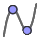
\includegraphics[width=0.0275\linewidth]{files/40px-Menu_view_algeb-122c1ab0ec365e77e9eae26ff7041249.png}

\textit{Graf} (ang. 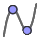
\includegraphics[width=0.0275\linewidth]{files/40px-Menu_view_algeb-122c1ab0ec365e77e9eae26ff7041249.png}

\textit{Graphing perspective}), ki omogoča risanje funkcij in geometrijskih objektov. Lahko jo vidite tudi spodaj:

\begin{framed}
\textbf{Opomba.}\\
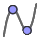
\includegraphics[width=0.0275\linewidth]{files/40px-Menu_view_algeb-122c1ab0ec365e77e9eae26ff7041249.png}

\textit{Graphing perspective} je eden izmed več prikazi, ki jih ponuja Geogebra. Vsaka aplikacija Geogebre je sestavljena iz različnih prikazov, tako da lahko ustvarimo gradiva za različne aplikacije.
Različne prikaze lahko izberemo s klikom na gumb 
\includegraphics[width=0.0275\linewidth]{files/16px-Menu-button-ope-f5b0cc09aa629bb7475641338f148b1b.png}

 \textit{Menu} v zgornjem levem kotu in nato izbiro možnosti 
\includegraphics[width=0.0275\linewidth]{files/16px-Menu-perspectiv-ce02b8b20d416cda63cc58e40cc62dbc.png}

 \textit{Perspectives}.
\end{framed}

Vsak prikaz ponuja različne \textit{poglede} (ang, \textit{views}).
Lahko jih dodamo ali odstranimo glede na naše potrebe s klikom na gumb 
\includegraphics[width=0.0275\linewidth]{files/16px-Menu-button-ope-f5b0cc09aa629bb7475641338f148b1b.png}

 \textit{Menu} v zgornjem levem kotu in nato izbiro možnosti 
\includegraphics[width=0.0275\linewidth]{files/16px-Menu-view.svg-f949496793bee1afbf5580c9151ff29f.png}

 \textit{View}.
Različni pogledi vključujejo:

\begin{itemize}
\item 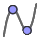
\includegraphics[width=0.0275\linewidth]{files/40px-Menu_view_algeb-122c1ab0ec365e77e9eae26ff7041249.png}

 \textit{Algebrsko okno} (ang. 
\includegraphics[width=0.7\linewidth]{files/16px-Menu_view_algeb-f43b4e7001b948efd7156019d70162e5.png}

\textit{Algebra}).
\item 
\includegraphics[width=0.7\linewidth]{files/16px-Menu_view_cas.s-ac920cb977e8fa51fa4cc9b2de0f21dc.png}

 \textit{Simbolno računanje} (ang. 
\includegraphics[width=0.7\linewidth]{files/16px-Menu_view_cas.s-ac920cb977e8fa51fa4cc9b2de0f21dc.png}

\textit{CAS}).
\item 
\includegraphics[width=0.7\linewidth]{files/16px-Menu_view_graph-07f951165e69080135ae4e0c7469a7db.png}

 \textit{Risalna površina} (ang. 
\includegraphics[width=0.7\linewidth]{files/16px-Menu_view_graph-07f951165e69080135ae4e0c7469a7db.png}

\textit{Graphics}).
\item 
\includegraphics[width=0.7\linewidth]{files/16px-Menu_view_graph-07f951165e69080135ae4e0c7469a7db.png}

 \textit{Grafika 2} (ang. 
\includegraphics[width=0.7\linewidth]{files/16px-Menu_view_graph-2e4bf4b6093ffe88df8ecbb808ff2af0.png}

\textit{Graphics 2}).
\item 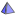
\includegraphics[width=0.7\linewidth]{files/16px-Perspectives_al-4b30a8dd240c5689614b0c4160650a7f.png}

 \textit{3d grafika} (ang. 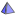
\includegraphics[width=0.7\linewidth]{files/16px-Perspectives_al-4b30a8dd240c5689614b0c4160650a7f.png}

\textit{3D Graphics}).
\item 
\includegraphics[width=0.7\linewidth]{files/16px-Menu_view_sprea-accffca900ee2847b6d4e16428ea9434.png}

 \textit{Preglednica} (ang. 
\includegraphics[width=0.7\linewidth]{files/16px-Menu_view_sprea-accffca900ee2847b6d4e16428ea9434.png}

\textit{Spreadsheet}).
\item 
\includegraphics[width=0.7\linewidth]{files/16px-Menu_view_proba-42fa17d822cb9c58be706d74d5141054.png}

 \textit{Računanje verjetnosti} (ang. 
\includegraphics[width=0.7\linewidth]{files/16px-Menu_view_proba-42fa17d822cb9c58be706d74d5141054.png}

\textit{Probability Calculator}).
\end{itemize}

Drugi vnosi nad gumbom 
\includegraphics[width=0.0275\linewidth]{files/16px-Menu-button-ope-f5b0cc09aa629bb7475641338f148b1b.png}

 \textit{Menu} omogočajo dostop do različnih orodij in nastavitev Geogebre, kot so:

\begin{itemize}
\item 
\includegraphics[width=0.0275\linewidth]{files/16px-Menu-file.svg-b74615e1101cba241695021ac4f1343d.png}

 \textit{Datoteka} (ang. 
\includegraphics[width=0.0275\linewidth]{files/16px-Menu-file.svg-b74615e1101cba241695021ac4f1343d.png}

\textit{File}): Ustvarjanje, odpiranje, shranjevanje in izvoz datotek.
\item 
\includegraphics[width=0.0275\linewidth]{files/16px-Menu-edit.svg-db315b9e8b33fcb7c2a004c62d0b43a2.png}

 \textit{Uredi} (ang. 
\includegraphics[width=0.0275\linewidth]{files/16px-Menu-edit.svg-db315b9e8b33fcb7c2a004c62d0b43a2.png}

\textit{Edit}): Razveljavi, ponovi, kopiraj, prilepi in druge osnovne funkcije urejanja.
\item 
\includegraphics[width=0.0275\linewidth]{files/16px-Menu-options.sv-ff60e1f4269388c4072d3fd2116dba4c.png}

 \textit{Nastavitev} (ang. 
\includegraphics[width=0.0275\linewidth]{files/16px-Menu-options.sv-ff60e1f4269388c4072d3fd2116dba4c.png}

\textit{Settings}): Prilagajanje nastavitev Geogebre, kot so jezika, velikosti pisave in drugih možnosti.
\item 
\includegraphics[width=0.7\linewidth]{files/16px-Menu-tools.svg-7308442ad87596c4ecdbba52b18fe152.png}

 \textit{Orodja} (ang. 
\includegraphics[width=0.0275\linewidth]{files/16px-Menu-tools.svg-7308442ad87596c4ecdbba52b18fe152.png}

\textit{Tools}): Dostop do različnih orodij za risanje in konstrukcije.
\item 
\includegraphics[width=0.0275\linewidth]{files/24px-Menu-help.svg-0cd4dfd2862bbf9cf5b3df3fd837509b.png}

 \textit{Pomoč} (ang. 
\includegraphics[width=0.0275\linewidth]{files/24px-Menu-help.svg-0cd4dfd2862bbf9cf5b3df3fd837509b.png}

\textit{Help and Feedback}): Dostop do dokumentacije, vadnic in podpore skupnosti Geogebra.
\item 
\includegraphics[width=0.0275\linewidth]{files/24px-Menu-account-48e0e0ba7557ab477eca8f9143328c18.png}

 \textit{Račun} (ang. 
\includegraphics[width=0.0275\linewidth]{files/24px-Menu-account-48e0e0ba7557ab477eca8f9143328c18.png}

 \textit{Account}): Prijava in odjava iz računa Geogebra.
\end{itemize}

\begin{framed}
\textbf{Opomba}\\
Geogebra se lahko uporablja v slovenskem jeziku, vmesnik je preveden, prav tako pa tudi ukazi, žal pa ni dokumentacije v slovenskem jeziku za ukaze (ki jih uporabljamo za ustvarjanje gradiva). Zaradi tega bomo vmesnik ohranili v angleščini, vendar upoštevajte, da če želite Geogebro uporabljati z otroki ali učenci, lahko jezik spremenite v meniju 
\includegraphics[width=0.0275\linewidth]{files/16px-Menu-options.sv-ff60e1f4269388c4072d3fd2116dba4c.png}

\textit{Settings}.
\end{framed}

Poleg gumba 
\includegraphics[width=0.0275\linewidth]{files/16px-Menu-button-ope-f5b0cc09aa629bb7475641338f148b1b.png}

 \textit{Menu}, pomembni del orodjarne so tudi:

\begin{figure}
\centering
\begin{tabular}{p{\dimexpr 0.500\linewidth-2\tabcolsep}p{\dimexpr 0.500\linewidth-2\tabcolsep}}
\toprule
\textit{Orodarne} (ang. \textit{Toolbar}): & 
\includegraphics[width=0.7\linewidth]{files/344px-Toolbar-Graphi-8fcf80f609483dd4257ab538ddc900ac.png}

 \\
\textit{Slog vrstica} (ang. \textit{Stylebar}): & 
\includegraphics[width=0.03\linewidth]{files/40px-Stylingbar_icon-dbbb2f8b79b58bbc677f198035a192ed.png}

 \\
\textit{Razveljavi} (ang. \textit{Undo}): & 
\includegraphics[width=0.03\linewidth]{files/24px-Menu-edit-undo.-77ee2960343222cccf74a59680031c65.png}

 \\
\textit{Ponovno naredi} (ang. \textit{Redo}): & 
\includegraphics[width=0.03\linewidth]{files/24px-Menu-edit-redo.-070e92ceaaa1277418463e1041b58e49.png}

 \\
\bottomrule
\end{tabular}
\end{figure}

\subsubsection{Orodje}

Geogebra ponuja širok nabor orodij za ustvarjanje in manipulacijo matematičnih objektov. Orodja so dostopna prek orodjarne (ang. \textit{Toolbar}), ki se nahaja običajno na vrhu zaslona.
Orodjarna je odvisna od izbranega prikaza in ponuja različna orodja glede na kontekst.
Za zdaj, mi bomo raziskali nekaj osnovnih orodij, ki so na voljo v privzetem prikazu 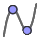
\includegraphics[width=0.0275\linewidth]{files/40px-Menu_view_algeb-122c1ab0ec365e77e9eae26ff7041249.png}

\textit{Graphing} in v prikazu 
\includegraphics[width=0.0275\linewidth]{files/16px-Menu_view_graph-07f951165e69080135ae4e0c7469a7db.png}

\textit{Graphics}, in sicer:


\includegraphics[width=0.7\linewidth]{files/344px-Toolbar-Graphi-8fcf80f609483dd4257ab538ddc900ac.png}

V nadelevanju opisujemo nekatere najpogosteje uporabljena orodja, celoten seznam orodij pa najdete v \href{https://geogebra.github.io/docs/manual/en/}{dokumentaciji Geogebre}.

Seveda, najlažji način za spoznavanje orodij je, da jih preizkusite sami v Geogebri!

\subsubsection{Vrstica za zamenjavo sloga}


\includegraphics[width=0.0275\linewidth]{files/40px-Stylingbar_icon-dbbb2f8b79b58bbc677f198035a192ed.png}

 \textit{Vrstica za zamenjavo sloga} (ang. \textit{Stylebar}) omogoča hitro spreminjanje grafičnih lastnosti izbranih objektov, kot so barva, debelina črte, slog črte in polnilo.
Ko izberete objekt v grafičnem oknu, se vrstica za zamenjavo sloga prikaže pod orodjarno in ponuja različne možnosti za prilagajanje videza izbranega objekta.
Možnosti so odvisne od vrste izbranega objekta, če ni objekta izbranega, vrstica za zamenjavo sloga prikaže možnosti sloga za pogled.

V vrstici za zamenjavo sloga se nahajajo samo osnovne možnosti, za dostop do naprednih možnosti sloga pa lahko kliknete na gumb 
\includegraphics[width=0.0225\linewidth]{files/32px-Settings.svg-c4703801fadb8667750afe6331c554d5.png}

 \textit{Nastavitve} (ang. \textit{Settings}), ki odpre pogovorno okno z več možnostmi za prilagajanje sloga izbranega objekta. Če ni izbranega objekta, gumb 
\includegraphics[width=0.0225\linewidth]{files/32px-Settings.svg-c4703801fadb8667750afe6331c554d5.png}

 \textit{Nastavitve} odpre pogovorno okno z možnostmi za prilagajanje sloga pogleda.

\subsubsection{Ukaze}

GeoGebra poleg grafičnih orodij ponuja tudi algebrske vnose in ukaze. Vsako orodje ima ustrezen ukaz, zato ga je mogoče uporabljati brez miške.

\begin{framed}
\textbf{Nasvet}\\
Dokumentacija za ukaze je v angleščini, zato je priporočljivo, da imate ukaze uporabite v angleščini.
Več o ukazih in njihovi uporabi najdete v \href{https://geogebra.github.io/docs/manual/en/}{dokumentaciji Geogebre}.
\end{framed}

\begin{framed}
\textbf{Opomba}\\
Vsaka orodoja ima svoj ukaz, obratno pa ne velja, obstajajo več ukazov kot orodij.
Večina uporabnikov Geogebra lahko brez težav dela z grafičnimi orodji, vendar moramo avtorji znati uporabljati ukaze. Tako bomo lahko delali hitreje in natančneje.
\end{framed}

Če hitro uporabimo ukaz, lahko ga vnesemo v \textit{Vrstico za vnos} (ang. \textit{Input Bar}), ki se običajno nahaja na dnu zaslona. Alternativno, lahko ukaze vnesemo tudi neposredno v grafično okno ali v 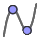
\includegraphics[width=0.0275\linewidth]{files/40px-Menu_view_algeb-122c1ab0ec365e77e9eae26ff7041249.png}

 \textit{Algebrsko okno} (ang. \textit{Algebra View}). Oboje lahko najdemo v meni ju 
\includegraphics[width=0.0275\linewidth]{files/32px-Menu-view.svg-287f1be47c2a7a168b1e84c64f1ec13c.png}

 \textit{Views}.

Naljažje način za spoznavanje ukazov je, da jih preizkusite sami v Geogebri!

\begin{framed}
\textbf{Nasvet}\\
Ko uporabite ukazi v Geogebri, je pomembno, da
upoštevate naslednje nasvete:

\begin{itemize}
\item Točke so definirane z velikimi črkami (npr. A, B, C), medtem ko so premice, daljice in krožnice definirane z malimi črkami (npr. a, b, c).
\item Pri vnosu koordinat točk uporabite oklepaje in vejice, npr. (2,3) za točko z $x$ koordinato 2 in $y$ koordinato 3.
\item Ukaz $v=(1,2)$ ne definira točke, ampak vektor z komponentama 1 in 2.
\item Uporabite  za samodejno dokončanje imen ukazov in objektov.
\item Uporabite  in  za navigacijo po zgodovini ukazov v vrstici za vnos.
\item Z gumbom 
\includegraphics[width=0.0225\linewidth]{files/24px-Menu-help.svg-0cd4dfd2862bbf9cf5b3df3fd837509b.png}

 \textit{Help} (sl. \textit{Pomoč}) (na desno od vrstice za vnos) lahko dostopate do dokumentacije Geogebre za ukaze.
\end{itemize}
\end{framed}

V Exercise~\ref{ex_GeogebraUkazi-1} ste se naučili

\begin{itemize}
\item Ustvariti geometrijske objekte z uporabo ukazov v vrstici za vnos.
\item Meriti kotov in dolžin in z uporabo orodje.
\item Prilagoditi besedilo z uporabo LaTeX formul.
\item Nastavitev \texttt{Starting point} za pozicioniranje besedila.
\end{itemize}


\bigskip
\centerline{\rule{13cm}{0.4pt}}
\bigskip

Geogebra nam omogoča vizualizacijo osnovnih geometrijskih konstrukcij in iskanje vzorcev v njih.
Na primer, pri konstrukciji v Exercise~\ref{ex_GeogebraUkazi-1} lahko opazimo, da je trikotnik $ABC$ vedno enakostraničen, ne samo za izbiro točko $A=(0,0)$ in $C=(4,0)$, ampak za katerokoli izbiro točk $A$ in $C$.
To lahko vidimo, če povlečemo točki $A$ in $C$ z orodjem 
\includegraphics[width=0.0225\linewidth]{files/32px-Mode_move.svg-b420ab97c3d398837a03b0709d9d93f2.png}

 \textit{Move}.
Opazimo da so dolžini stranici $AB$, $BC$ in $CA$ vedno enaki.
V Geogebri je to znano kot \textbf{test vlečenja} (ang. \textit{dragging test}), ki nam pomaga pri odkrivanju in dokazovanju geometrijskih lastnosti.

V prešnji konstrukciji smo uporabili \textbf{test vlečenja} (ang. \textit{dragging test}), ki nam pomaga pri odkrivanju in dokazovanju, da je trikotnik $ABC$ vedno enakostraničen.
S testom vlečenja lahko tudi vidimo, da so vsi koti v enakostraničnem trikotniku enaki in merijo $60^\circ$. To sledi iz dejstva, da je vsota notranjih kotov v trikotniku vedno $180^\circ$ in da so vsi trikotniki enakostranični.

\subsubsection{Algebrsko okno, proste točke vs. odvisne točke in kontrolni okvirček}

Vrstica za vnos ni edini način za interakcijo z Geogebro z uporabo ukazov.
Lahko uporabimo tudi 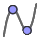
\includegraphics[width=0.0275\linewidth]{files/40px-Menu_view_algeb-122c1ab0ec365e77e9eae26ff7041249.png}

 \textit{Algebrsko okno} (ang. \textit{Algebra View}), ki prikazuje seznam vseh objektov v konstrukciji skupaj z njihovimi lastnostmi in vrednostmi.

Upoštevajte, da so točke \texttt{A} in \texttt{B} \textbf{proste točke} (ang. \textit{free points}), ker jih lahko premikamo kjerkoli v grafičnem oknu.
Vse ostale točke v konstrukciji so \textbf{odvisne točke} (ang. \textit{dependent points}), ker so določene z drugimi objekti v konstrukciji in se premikajo glede na spremembe teh objektov.
Proste točke so običajno modre barve, medtem ko so odvisne točke sive barve.
Seveda, to lahko spremenimo z uporabo vrstice za zamenjavo sloga ali v nastavitvah objekta, in torej barva ni zanesljiv indikator vrste točke.
V algebrskem oknu lahko vidimo katere objekte so proste in katere odvisne, saj so uporabimo gump \textit{Sort by} in torej \textit{Dependency} v vrstico za zamenjavo sloga algebrskega okna.


\bigskip
\centerline{\rule{13cm}{0.4pt}}
\bigskip

Kot smo videli, lahko uporabimo orodje 
\includegraphics[width=0.0275\linewidth]{files/32px-Mode_showhideob-4d2ce0e2e5642356a4a38fcbc8665f16.png}

 \textit{Show/Hide Object} za prikaz ali skrivanje objektov v grafičnem oknu.
To lahko storimo tudi v algebrskem oknu, kjer lahko kliknemo na krog levo od imena objekta za prikaz ali skrivanje objekta.
Poleg tega, lahko uporabimo tudi kontrolni okvirček (ang. \textit{checkbox}), ki ga lahko ustvarimo z orodjem 
\includegraphics[width=0.0275\linewidth]{files/32px-Mode_showcheckb-13e0b16b7961c33cdddba6a813116e81.png}

 \textit{Check Box} ali z ukazom \texttt{CheckBox()}.
Kontrolni okvirček vstavirte \textit{Check Box} v grafično okno in booleansko vrednost v algebrskem oknu.
Nato lahko uporabimo to vrednost za nadzor vidljivosti drugih objektov v konstrukciji.

\subsubsection{Izvoz konstrukcij kot slike.}

Lahko izvozimo naše konstrukcije iz Geogebre kot slike v različnih formatih, kot so \texttt{PNG}, \texttt{SVG} ali \texttt{PDF}.
Za izvoz konstrukcije kot slike, sledite tem korakom:

\begin{enumerate}
\item Pojdite na meni 
\includegraphics[width=0.0275\linewidth]{files/16px-Menu-file.svg-b74615e1101cba241695021ac4f1343d.png}

 \textit{File} in izberite 
\includegraphics[width=0.0275\linewidth]{files/24px-Menu-download.s-5fe900c8334923e022076eea13194034.png}

 \textit{Download as...}.
\item V pogovornem oknu izberite želeni format slike (npr. \texttt{.png}, \texttt{.svg} ali \texttt{.pdf}).
\item Posebni format je \texttt{PGF/TikZ}, ki omogoča izvoz konstrukcije kot kode, ki jo lahko uporabimo v LaTeX dokumentih.
\end{enumerate}

\subsubsection{Vaje}\label{07_geogebraUvod_vaje}

\begin{itemize}
\item Exercise~\ref{ex_GeogebraAccount}: Ustvarjanje računa Geogebra.
\item Exercise~\ref{ex_GeogebraTools}: Vaje za spoznavanje orodij Geogebre.
\item Exercise~\ref{ex_Stylebar}: Vaje za uporabo vrstice za zamenjavo sloga.
\item Exercise~\ref{ex_GeogebraUkazi-1}: Vaje za spoznavanje ukazov Geogebre.
\item Exercise~\ref{ex_dokazTrikotnik}: Vaje za dokazovanje lastnosti trikotnika z uporabo Geogebre.
\item Exercise~\ref{ex_TrikotnikKot}: Vaje za dokazovanje vsote notranjih kotov v trikotniku z uporabo Geogebre.
\item Exercise~\ref{ex_pentagram}: Vaje za ustvarjanje petkotnika in zvezde z uporabo Geogebre.
\item Exercise~\ref{ex_checkbox}: Vaje za uporabo kontrolnega okvirčka za nadzor vidljivosti objektov v Geogebri.
\end{itemize}

\subsection{Dinamična geometrija z GeoGebro}

V poglavju \href{/geogebrauvod}{GeoGebra: Uvod} smo spoznali osnove dela z GeoGebro. V tem poglavju bomo raziskali, kako ustvariti animacije in dinamične konstrukcije z uporabo GeoGebre.

\subsubsection{Točka na objektu}

Najlažje način za ustvarjanje dinamične konstrukcije je uporaba točke, ki je vezana na drug objekt. Točko lahko postavimo na premico, krožnico ali katerikoli drug objekt, kar omogoča, da se točka premika znotraj omejitve tega objekta.

Ko ustvarimo točko na krivulji (kot so premice, krožnice, graf funkcij itd.), lahko to točko animiramo. To naredimo tako, da izberemo točko in kliknemo na gumb 
\includegraphics[width=0.02\linewidth]{files/18px-Nav_play_circle-74635dc1a7e6d0a614249108e021d156.png}

 \textit{Play} v algebrskem oknu ali uporabimo ukaz \texttt{StartAnimation(\textless točka\textgreater )}. S tem se bo točka začela premikati po objektu, na katerem je bila ustvarjena.

Na žalost GeoGebra ne omogoča animacije točk na daljših objektih, kot so mnogokotniki. Vendar pa lahko ustvarimo drsnike, ki nam omogočajo nadzor nad položajem točke na takšnih objektih s pomočjo parametra.

\subsubsection{Drsniki}

V resnični, drsniki so samo orodja za spreminjanje vrednosti spremenljivk. Vendar pa so zelo uporabni pri ustvarjanju dinamičnih konstrukcij, saj nam omogočajo, da spreminjamo vrednosti in opazujemo, kako se konstrukcija spreminja.

Drsniki imajo tri glavne lastnosti: \texttt{Min} (minimalna vrednost), \texttt{Max} (maksimalna vrednost) in \texttt{Increment} (prirastek). Te lastnosti določajo obseg vrednosti, ki jih drsnik lahko zavzame, in kako hitro se vrednost spreminja, ko premikamo drsnik.

Za ustvarjanje drsnika lahko uporabimo orodje 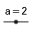
\includegraphics[width=0.0275\linewidth]{files/32px-Mode_slider.svg-e15eadebbb4f9101af436526f2609a2c.png}

 \textit{Slider} (\textit{Drsnik}) in dobimo okno za nastavitev lastnosti drsnika. Drsnike lahko ustvarimo tudi z vnosom imena spremenljivke v vnosno vrstico, na primer \texttt{a=5}, kar ustvari spremenljivk z imenom \texttt{a} in začetno vrednostjo 5. Nato lahko kliknemo na tri pike poleg imena spremenljivke v algebrskem oknu in nato \textit{Create slider} (\textit{Ustvari drsnik}). To ustvari drsnik z privzetimi lastnostmi (\texttt{Min=-5}, \texttt{Max=5}, \texttt{Increment=0.1}), ki jih lahko spremenimo z dvojnim klikom na drsnik (v grafičnem pogledu) ali z desnim klikom na ime spremenljivke v algebrskem oknu in izbiro \textit{Settings} (\textit{Nastavitve}). V oknu z nastavitvami lahko spremenimo lastnosti drsnika, kot so \texttt{Min}, \texttt{Max} in \texttt{Increment}, in tudi druge lastnosti, kot so barva, slog in vidnost.

Drsniki lahko tudi uporabimo za ustvarjanje animacij. To naredimo tako, da izberemo drsnik in kliknemo na gumb 
\includegraphics[width=0.02\linewidth]{files/18px-Nav_play_circle-74635dc1a7e6d0a614249108e021d156.png}

 \textit{Play} v algebrskem oknu ali uporabimo ukaz \texttt{StartAnimation(\textless drsnik\textgreater )}. S tem se bo vrednost drsnika začela spreminjati samodejno z določenim prirastkom, kar omogoča ustvarjanje animacij v konstrukciji.

\subsubsection{Zaporedja}

Ukaz \texttt{Sequence()} omogoča ustvarjanje zaporedij objektov v GeoGebri. Splošna oblika ukaza je \texttt{Sequence(\textless izraz\textgreater , \textless spremenljivka\textgreater , \textless začetek\textgreater , \textless konec\textgreater , \textless korak\textgreater )}, kjer \texttt{\textless izraz\textgreater } je izraz (običajno ukaz GeoGebre), ki ga želimo ponoviti, \texttt{\textless spremenljivka\textgreater } je spremenljivka, ki se spreminja v zaporedju, \texttt{\textless začetek\textgreater } in \texttt{\textless konec\textgreater } določata obseg vrednosti za spremenljivko, in \texttt{\textless korak\textgreater } določa, za koliko se spremenljivka poveča v vsakem koraku.
Variantne ukaza so:

\begin{itemize}
\item \texttt{Sequence(\textless konec\textgreater )} - ustvari zaporedje števil od 1 do \texttt{\textless konec\textgreater }.
\item \texttt{Sequence(\textless začetek\textgreater ,\textless konec\textgreater )} - ustvari zaporedje števil od \texttt{\textless začetek\textgreater } do \texttt{\textless konec\textgreater }.
\item \texttt{Sequence(\textless izraz\textgreater , \textless spremenljivka\textgreater , \textless začetek\textgreater , \textless konec\textgreater )} - ustvari zaporedje z privzetim korakom 1.
\end{itemize}

Ukaz \texttt{Sequence()} ustvari zaporedje objektov, če hočemo izbrati posamezne objekte iz zaporedja, lahko uporabimo ukaz\texttt{Element(\textless zaporedje\textgreater , \textless indeks\textgreater )}, kjer \texttt{\textless zaporedje\textgreater } je zaporedje objektov in \texttt{\textless indeks\textgreater } je indeks objekta, ki ga želimo izbrati (indeksi se začnejo pri 1).

Če hočemo izgraditi več objektov (namesto zaporedje objektov), lahko uporabimo naslednje način:

\begin{itemize}
\item Ustvarimo zaporedje objektov z ukazom \texttt{Sequence()}, npr. \texttt{kroznice = Sequence(Circle((0,0), i), i, 1, 5)}, ki ustvari zaporedje krožnic s polmeri od 1 do 5.
\item Nato uporabimo ukazi \texttt{Sequence()} in \texttt{Element()} za ustvarjanje zaporedja ukazov, npr. \texttt{kroU=Sequence("K\_\{"+i+"\} = Element(kroznice, "+i+")", i, 1, 5)}, ki ustvari zaporedje ukazov za vsako krožnico v zaporedju z imenom \texttt{krogU}. V tem primeru ustvarimo ukaze \texttt{K\_\{1\} = Element(kroznice, 1)}, \texttt{K\_\{2\} = Element(kroznice, 2)}, itd.
\item Na koncu uporabimo ukaz \texttt{Execute()} za izvedbo vsakega ukaza.
\end{itemize}

Ta način lahko uporabimo za ustvarjanje zaporedje ukazov, da ni nujno ustvariti objekte. Na primer z ukazom
\texttt{barv=Sequence("SetDynamicColor(L\_\{"+i+"\}, random(), random(), random(), 0.5)", i, 1, 40)}, ustvarimo zaporedje ukazov za nastavitev naključne barve za vsako daljico, nato pa z ukazom \texttt{Execute(barv)} izvedemo te ukaze in tako nastavimo barve za vse daljice naenkrat. \textit{Pozkusite to sami}!


\bigskip
\centerline{\rule{13cm}{0.4pt}}
\bigskip

Zaporedje in drsniki postanejo zelo močna orodja, ko jih kombiniramo skupaj. Na primer, lahko ustvarimo drsnik, ki določa število objektov v zaporedju, in nato uporabimo ta drsnik za ustvarjanje dinamične konstrukcije, ki se spreminja glede na vrednost drsnika. Ta način bomo raziskali v naslednjih vajah.

\subsubsection{Vaje}\label{08_geogebraDinGeometrija_vaje}

\begin{itemize}
\item Exercise~\ref{ex-paralelogram} - Ustvarite dinamični paralelogram in opazujte, kako se spreminja njegova površina.
\item Exercise~\ref{ex-drsniki-1} - Ustvarite premico z drsniki za naklon in presečišče z osjo y ter opazujte, kako se spreminja premica.
\item Exercise~\ref{ex-drsniki-2} - Ustvarite dinamično konstrukcijo, ki prikazuje veljavnost trikotne neenakosti s pomočjo drsnikov in dinamičnih barv.
\item Exercise~\ref{ex-drsniki-3} - Ustvarite animacijo z uporabo drsnikov za premikanje točk v ravnini.
\item Exercise~\ref{ex-drsniki-4} - Ustvarite dinamično konstrukcijo za seštevanje dveh celih števil z uporabo drsnikov.
\item Exercise~\ref{ex_sequences-1} - Ustvarite zaporedje točk na krožnici z uporabo ukaza \texttt{Sequence()}.
\item Exercise~\ref{ex_sequences-2} - Uporabite ukaz \texttt{Sequence()} za ustvarjanje vzorca premic v GeoGebri.
\item Exercise~\ref{ex_sequences-3} - Uporabite ukazi \texttt{Element()} in \texttt{Execute()} za ustvarjanje posamezni objektov iz zaporedje.
\end{itemize}

%  - [Vaje %s](#ex_sequences-4) - Ustvarite dinamično konstrukcijo za množenje dveh celih števil z uporabo drsnikov in ukaza `Sequence()`.

%  - [Vaje %s](#ex_pythagoras) - Ustvarite konstrukcijo, ki prikazuje dokaz Pitagorovega izreka z uporabo drsnikov.

%  - [Vaje %s](#ex-circleArea) - Ustvarite dinamično konstrukcijo za izračun površine kroga s pomočjo drsnika za polmer kroga.

%  :::{solution} ex_sequences-4
% :class: tip dropdown
% Lahko uporabite naslednje korake za ustvarjanje te konstrukcije:
% 1. Ustvarite drsnika `a` in `b` z lastnostmi: `Min=1`, `Max=10`, `Increment=1`.
% 2. Upoštevajte da ukaz `Sequence((i,j),i,1,a)` ustvari zaporedje točk v dani vrstici z drugim koordinato `j`. 
% 3. Uporabite ukaz `točke=Sequence(Sequence((i,j),i,1,a),j,1,b)` za ustvarjanje zaporedja točk v pravokotniku z dolžino `a` in širino `b`.
% 5. Z uporabo ukaza `FormulaText("$"+a+"\times"+b+"="+(a*b)+"$")` ustvarite dinamično besedilo, ki prikazuje rezultat množenja `a` in `b`.
% 6. Uredite položaj besedila in slog po želji.
% 
% Lahko odprete to konstrukcijo v GeoGebri [tukaj](https://www.geogebra.org/classic/nkczhbrd).
% 
% :::

\subsection{Analiza z GeoGebro}

\subsubsection{Sledovi (traces in loci)}

Sledovi (ang. \textit{traces}) in loci (ang. \textit{loci}) so uporabna orodja v GeoGebri za analizo geometrijskih in funkcijskih lastnosti. Sledovi omogočajo sledenje poti točke, ki se premika glede na druge objekte, medtem ko loci prikazujejo množico točk, ki izpolnjujejo določene pogoje.
Razlika med sledovi in loci je v tem, da sledovi prikazujejo pot posamezne točke, medtem ko loci prikazujejo celotno množico točk, ki izpolnjujejo določene pogoje. Najlaže je, da to ponazorimo z naslednjo konstrukcijo:

\begin{framed}
\textbf{Glej tudi}\\
Peucellier-Lipkinov mehanizem je opisan tudi na \href{https://en.wikipedia.org/wiki/Peaucellier\%E2\%80\%93Lipkin\_linkage}{Wikipediji} (ang.). To je mehanizem, ki pretvarja krožno gibanje v ravno linijsko gibanje. Uporablja se lahko za risanje ravnih črt brez uporabe ravnila, poleg tega, lahko tudi uporabimo za risanje krožnic brez uporabe kompasa.
\end{framed}

Lahko tudi uporabimo orodja 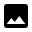
\includegraphics[width=0.0275\linewidth]{files/32px-Mode_image.svg-4ad09c46e3d21949ce372e4d0648d1bc.png}

 \textit{Image} (\textit{Slika}) za uvoz slike mačke in nato sledimo poti določene točke na sliki. To je prikazano v naslednjem konstrukciji:

Če želite, lahko to konstrukcijo odprete v GeoGebri \href{https://www.geogebra.org/classic/hmycsecx}{tukaj}. \textbf{Poskusite sami!}, Če želite, lahko uporabite moje slike: \href{/wall-2f1cf445f820b17acd3ef1477ed55808.png}{wall.png} in \href{/cat-047eeea8d3ff40424daab3c0f825a5f0.png}{cat.png}.

\subsubsection{Funkcije}

GeoGebra ima veliko vnaprerej določenih funkcij, ki jih lahko uporabimo za analizo. Nekatere izmed teh funkcij vključujejo: \texttt{sin()} (sinus), \texttt{cos()} (kosinus), \texttt{tan()} (tangens), \texttt{exp()} (eksponentna funkcija), \texttt{ln()} (naravni logaritem) in še več. (celoten seznam (v ang.) \href{https://geogebra.github.io/docs/manual/en/Predefined\_Functions\_and\_Operators/}{tukaj}) Te funkcije lahko uporabimo za ustvarjanje grafov in izvajanje različnih analiz.

Za uporaba funkcije v GeoGebri, preprosto vnesite ime funkcije, sledeno z oklepaji, ki vsebujejo argumente funkcije. Na primer, za risanje grafa funkcije $f(x) = \sin(x)$, vnesite \texttt{f(x) = sin(x)} v vhodno vrstico in pritisnite .

Lahko tudi ustvarimo funkcije, ki so odvisne od drugih objektov v GeoGebri. Na primer, z ukazom \texttt{g(x) = ax\^3 + bx\^2 + cx + d} lahko ustvarimo funkcijo, ki je odvisna od spremenljivk \texttt{a}, \texttt{b},\texttt{c} in \texttt{d}. Te spremenljivke lahko nato nastavimo na določene vrednosti ali jih povežemo z drsniki za dinamično prilagajanje funkcije.

Nekatera pomembna orodja za delo s funkcijami so:

\begin{itemize}
\item Ukaz \texttt{Roots(\textless funkcija\textgreater , \textless min x\textgreater , \textless max x\textgreater  )} najde ničle funkcije na intervalu $[\min x, \max x]$.
\item Ukaz \texttt{Max(\textless funkcija\textgreater , \textless min x\textgreater , \textless max x\textgreater )} najde maksimum funkcije na določenem intervalu.
\item Ukaz \texttt{Min(\textless funkcija\textgreater ,\textless min x\textgreater , \textless max x\textgreater )} najde minimum funkcije na intervalu $[\min x, \max x]$.
\end{itemize}

Če hitro želimo najti nekatere lastnosti funkcije, lahko uporabimo orodje 
\includegraphics[width=0.0275\linewidth]{files/32px-Mode_functionin-5eeb13f1a6b97d3950fb00eba6b0d8dc.png}

 \textit{Function Inspector} (\textit{Lastnosti funkcije}). To orodje nam omogoča hitro analizo funkcije in izračun njenih lastnosti, kot so ničle, ekstremi, infleksijske točke in še več.

Ko delamo s funkcijami v LaTeXu, je lahko koristno, da uredimo funkcije, s katerimi delamo. Za to, lahko uporabimo orodja 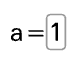
\includegraphics[width=0.0275\linewidth]{files/input-1126993cec2deafac9e4387fbf62c0c6.png}

 \textit{Input box} (\textit{Vhodno polje}). Ko ustvarimo vhodno polje, dobimo okno kjer določamo objekt, ki ga želimo prikazati in urejati \textit{Linked Object} (\textit{Povezani objekt}) in \textit{Caption} (\textit{Naslov}), ki bo prikazan poleg vhodnega polja.

\subsubsection{Odvodi in integrali}

\subsubsection{Polarni krivulje}

GeoGebra omogoča tudi risanje in analizo polarnih krivulj. Polarne krivulje so definirane z enačbami v polarnih koordinatah, kjer je vsaka točka določena z razdaljo od izhodišča (polmer) in kotom glede na pozitivno smer osi $x$.

Poleg tega, lahko prikažemo polarno omrežje v grafičnem oknu z klikom na 
\includegraphics[width=0.0275\linewidth]{files/40px-Stylingbar_icon-dbbb2f8b79b58bbc677f198035a192ed.png}

 \textit{Vrstica za zamenjavo sloga}, nato na 
\includegraphics[width=0.0275\linewidth]{files/network-bc241b4229fc5aeeee9f8a77efbc8d93.png}

 \textit{Show grid} (\textit{Omrežje}) in izberemo možnost 
\includegraphics[width=0.0275\linewidth]{files/polarnetwork-e67d0ef442577a3ded203720da15d499.png}

\textit{Polar Grid} (\textit{Polarno omrežje}).

\subsubsection{Parametrične krivulje}

Polarne krivulje so posebna vrsta parametričnih krivulj, kjer je polmer funkcija kota. Vendar pa lahko ustvarimo tudi splošne parametrične krivulje v GeoGebri z uporabo ukaza \texttt{Curve}. Ta ukaz omogoča definiranje krivulje z uporabo dveh funkcij, ki določata $x$ in $y$ koordinate glede na parameter $t$. Na primer, ukaz \texttt{Curve((cos(t), sin(t)), t, 0, 2*$\pi$)} ustvari enoto krožnico.

%  :::{exercise}
% :label: ex-paramentric
% 
% Ustvarite datoteko GeoGebra, ki prikazuje parametrično krivuljo.
% 
% 1. Ustvarite spremenljivki `max_t` in `min_t`.
% 2. Ustvarite funkciji za $x(t)$ in $y(t)$.
% 3. Ustvarite vhodno polje za `max_t` in `min_t`, da lahko spreminjate interval parametra $t$.
% :::

%  ```{margin}
% [Seznam vaj](_vaje)
% ```
% 
% :::{solution} ex-label
% :class: tip dropdown
% :::

%  ```{margin}
% [Seznam vaj](#vaje_geogebraAnaliza)
% ```
% 
% :::{solution} ex-polarni
% :class: tip dropdown
% :::

\subsubsection{Vaje}\label{vaje_geogebraAnaliza}

\begin{itemize}
\item Exercise~\ref{ex-peaucellier} Ustvarite Peaucellier-Lipkinov mehanizem v GeoGebri in analizirajte sled točke $F$.
\item Exercise~\ref{ex-cat} Kako se premika mačka, ko se lestev zdrsne po tleh?
\item Exercise~\ref{ex-functions-1} Ustvarite funkcijo in analizirajte njene lastnosti z orodji GeoGebre.
\item Exercise~\ref{ex-odvod-def} Ustvarite konstrukcijo v GeoGebri, ki omogoča prikaz definicije odvoda funkcije.
\item Exercise~\ref{ex-odvod} V konstrukciji iz prejšnje vaje, dodajte možnost za prikaz grafa odvoda funkcije.
\item Exercise~\ref{ex-integral} Ustvarite konstrukcijo v GeoGebri, ki omogoča prikaz določenega integrala funkcije med točkama $a$ in $b$.
\item Exercise~\ref{ex-polarni} Ustvarite polarne krivulje in analizirajte njihove lastnosti z orodji GeoGebre.
\end{itemize}

\subsection{Tridimenzionalna geometrija z GeoGebro}

GeoGebra 3D omogoča delo s tridimenzionalnimi objekti in njihovo vizualizacijo. V tem poglavju bomo raziskali osnovne funkcije GeoGebre 3D ter kako jih uporabiti za ustvarjanje in analizo tridimenzionalnih geometrijskih oblik.

Za delo v GeoGebri 3D moramo najprej preklopiti na 3D pogled. To storimo tako, da iz menija izberemo ``Perspectives'' in nato ``3D Graphics''. Prikaz ``3D Graphics'' vključuje tridimenzionalno koordinatno mrežo, ki nam omogoča ustvarjanje in manipulacijo 3D objektov, in tudi algebrsko okno, kjer lahko vidimo seznam vseh ustvarjenih objektov in njihovih lastnosti, podoben kot v 2D pogledu.

Točke v 3D prostoru ustvarimo z orodjem 
\includegraphics[width=0.0275\linewidth]{files/32px-Mode_point.svg-dc60e7c4e18f1e71b10806da1e7f4086.png}

 \textit{Point} (\textit{Točka}). Kliknemo na orodje in nato v 3D prostoru izberemo lokacijo, kjer želimo postaviti točko. Za to, moramo najprej določiti koordinate $x$ in $y$ v ravnini (sivi ravnini na 3D prikazu), nato pa določimo višino $z$ tako, da povlečemo točko navzgor ali navzdol. Ko ustvarimo točko, se njene koordinate prikažejo v algebrskem oknu. Alternativno lahko točko ustvarimo tudi z vnosom njenih koordinat v algebrsko okno, na primer \texttt{A = (2, 3, 4)}.

Podobno, za premikanje točk v 3D prostoru uporabimo orodje 
\includegraphics[width=0.0275\linewidth]{files/32px-Mode_move.svg-b420ab97c3d398837a03b0709d9d93f2.png}

 \textit{Move} (\textit{Premakni}). Nato lahko preklapljate med dvema načinoma s ponavljajočim klikom na točko, medtem ko je orodje aktivno: premikanje po ravnini (vzporedno v sivo ravnino) in premikanje navpično (v smeri osi $z$).

Najlažje način za učenje orodje je, da jih raziskujete.

\subsubsection{Točke in krogle}

Včasih je težko vse videti v 3D prostoru. Priporočamo, da eksperimentirate z različnimi pogledi in orodji za navigacijo v GeoGebri 3D. Vse najdete v 
\includegraphics[width=0.0275\linewidth]{files/32px-Stylingbar_icon-da79c17f9245fd7a577de157b0762fe4.png}

 \textit{Styling bar} (\textit{Vrstici za spremenite sloga pogleda}). Če želite ročno spremeniti pogled, uporabite orodje 
\includegraphics[width=0.0275\linewidth]{files/24px-Mode_rotateview-1ba2062ced630b55f4498b7eaa56a439.png}

 \textit{Rotate View} (\textit{Zasukaj pogled}) ali orodje 
\includegraphics[width=0.0275\linewidth]{files/32px-Mode_translatev-ebd873d304cfefb875a2544da650518a.png}

 \textit{Translate View} (\textit{Premakni pogled}).

\subsubsection{Premice in ravnine}

\subsubsection{Poliedri in drugi 3D objekti}

\subsubsection{Rotacijska ploskev}

Drugi način za prikaz rotacijske ploskve je z orodjem 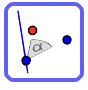
\includegraphics[width=0.0275\linewidth]{files/rotateAxis-2d3ed1b82acb9e1cff94634c58c97d2d.png}

 \textit{Rotate around Line} (\textit{Vrtenje okoli premice}).

\subsubsection{Funkcije z več spremenljivkami.}

\subsubsection{Vaje}\label{10_geogebra3D_vaje}

\begin{itemize}
\item Exercise~\ref{ex-spheres}: Ustvarite dve krogli v GeoGebri 3D in raziskujte njihovo presečišče.
\item Exercise~\ref{ex-distance}: Kako izmeriti razdaljo medo točkama v GeoGebri 3D?
\item Exercise~\ref{ex-cube}: Ustvarite kocko in ravnino v GeoGebri 3D ter poiščite njihovo presečišče.
\item Exercise~\ref{ex-polyhedra}: Ustvarite različne poliedre in 3D oblike v GeoGebri 3D.
\item Exercise~\ref{ex-rotational-surfaces}: Ustvarite rotacijske ploskve v GeoGebri 3D z vrtenjem daljic in krožnic okoli osi.
\item Exercise~\ref{ex-rotate-funkcije}: Ustvarite rotacijske ploskve z vrtenjem grafov funkcij okoli osi v GeoGebri 3D.
\item Exercise~\ref{ex-multivariable-functions}: Raziščujte funkcije z več spremenljivkami v GeoGebri 3D.
\end{itemize}

\subsection{GeoGebra: Izvoz in ustvarjanje učnih gradiv}

V izdelavi.

\section{SageMath}

\subsection{SageMath: Uvod}

\paragraph{Kaj je SageMath (SageMath)?}

\begin{itemize}
\item SageMath (na kratko Sage) je brezplačen odprtokodni programski sistem za matematiko.
\item Lahko si ga predstavljate kot Phyton na matematičnih steroidih.
\item Poslanstvo sistema SageMath je ustvariti učinkovito brezplačno odprtokodno alternativo sistemom Magma, Maple, Mathematica in Matlab.
\end{itemize}

\begin{framed}
\textbf{Glej tudi}\\
SageMath se pogosto uporablja in na spletu je na voljo veliko gradiva. Navajam nekaj najuporabnejših virov.

\begin{itemize}
\item SageMath Documentation: \href{https://doc.sagemath.org/}{https://doc.sagemath.org/}
\item SageMath Reference Manual: \href{https://doc.sagemath.org/html/en/reference/index.html}{https://doc.sagemath.org/html/en/reference/index.html}
\item A tour of SageMath: \href{https://doc.sagemath.org/html/en/a\_tour\_of\_sage/}{https://doc.sagemath.org/html/en/a\_tour\_of\_sage/}
\item Introductory SageMath tutorial: \href{https://doc.sagemath.org/html/en/prep/Intro-Tutorial.html}{https://doc.sagemath.org/html/en/prep/Intro-Tutorial.html}
\item SageMath tutorial: \href{https://doc.sagemath.org/html/en/tutorial/index.html}{https://doc.sagemath.org/html/en/tutorial/index.html}
\item SageMath thematic tutorial: \href{https://doc.sagemath.org/html/en/thematic\_tutorials/index.html}{https://doc.sagemath.org/html/en/thematic\_tutorials/index.html}
\item SageMath repository of interacts (interaktivni programčki): \href{https://wiki.sagemath.org/interact}{https://wiki.sagemath.org/interact}
\item SageMath quickref cards (reference za pomoč): \href{https://wiki.sagemath.org/quickref}{https://wiki.sagemath.org/quickref}
\end{itemize}
\end{framed}

\paragraph{Kako uporabljamo SageMath?}

SageMath lahko uporabljate na več načinov, vsak od njih ponuja različno raven nadzora in različne funkcije. Glavni načini uporabe so:

\begin{itemize}
\item \textbf{SageCell} \href{https://sagecell.sagemath.org/}{https://sagecell.sagemath.org/} Zelo uporabno za enostavne in hitre naloge.
\item \textbf{Lokalna namestitev}. Ni priporočljivo za začetnike. Če nimate izkušenj z nameščanjem programske opreme, je to lahko nekoliko zapleteno. Poleg tega skoraj nikoli ni potrebna. Edini dober razlog za lokalno namestitev programa SageMath je, da nimate dostopa do interneta.
\item \textbf{Interaktivni programčki}. Podobno kot apleti GeoGebre. Za uporabo interaktivnih programčkov ni treba imeti predznanja. Za njihovo ustvarjanje pa potrebujete napredno poznavanje programa SageMath, ki presega vsebine tega predmeta.
\item \textbf{\href{http://CoCalc.com}{CoCalc.com}} \url{https://cocalc.com/}. S preprostimi besedami, CoCal je za SageMath, kar je Overleaf za LaTeX.
\end{itemize}

\paragraph{SageMath na CoCalcu}

Obstajajo različne načine za uporabo SageMath, najpogosteje so:

\begin{itemize}
\item Na ukazni vrstici (terminalu). Ta način je primeren za napredne uporabnike in ni priporočljiv za začetnike. V tem primeru, SageMath deluje podobno kot običajen programski jezik, ukaze napišemo v terminal in dobimo rezultate. Ukazna vrstica običajno izgleda kot Figure~\ref{fig-terminal}.
\end{itemize}

\begin{figure}[!htbp]
\centering
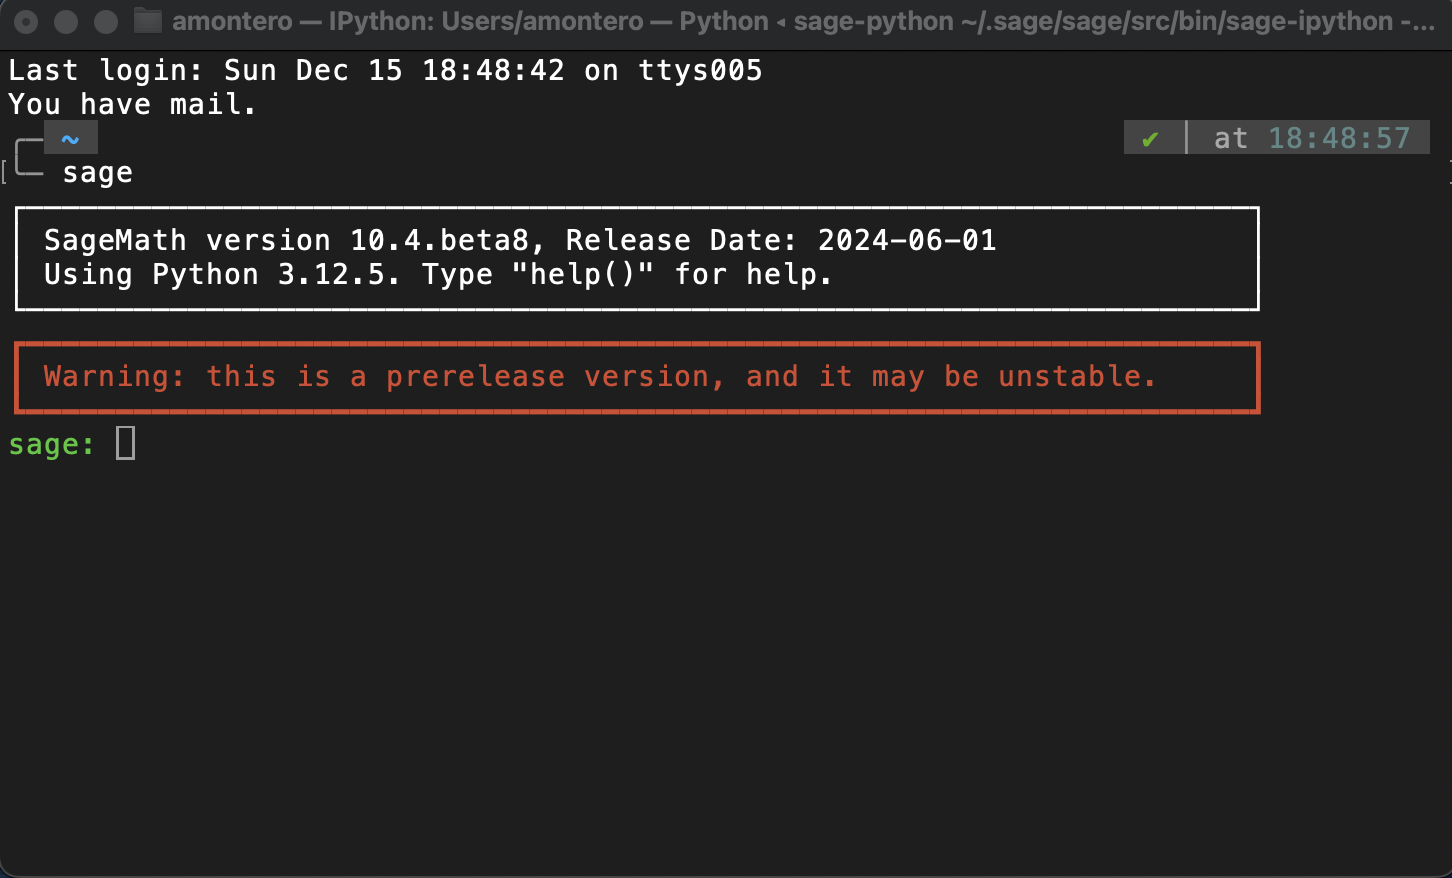
\includegraphics[width=0.5\linewidth]{files/terminal-e0334a7d9dbbd6f7e95e80a76bc04315.png}
\caption[]{Ukazna vrstica SageMath}
\label{fig-terminal}
\end{figure}

\begin{itemize}
\item Scripting: Kodo napišemo v besedilno datoteko in jo nato zaženete v ukazni vrstici. Ta način je prav tako primeren za napredne uporabnike in ni priporočljiv za začetnike, saj zahteva poznavanje osnov programiranja.
\item \textbf{Interaktivno v zvezku (Jupyter Notebook)}. Ta način je najbolj primeren za začetnike in je tisti, ki ga bomo uporabljali v tem predmetu. SageMath lahko uporabljamo v zvezkih Jupyter, ki omogočajo kombiniranje besedila, matematičnih izrazov in kode v enem dokumentu. Zvezki so zelo uporabni za učenje, raziskovanje in dokumentiranje matematičnih izračunov. V tem predmetu bomo uporabljali CoCalc, spletno platformo, ki omogoča uporabo SageMath v zvezkih Jupyter brez potrebe po lokalni namestitvi.
\end{itemize}

V beležnici Jupyter imamo dve vrsti celic: \textit{Code} (koda) in \textit{Text} (besedilo) (glej Figure~\ref{fig-celice}).

\begin{figure}[!htbp]
\centering
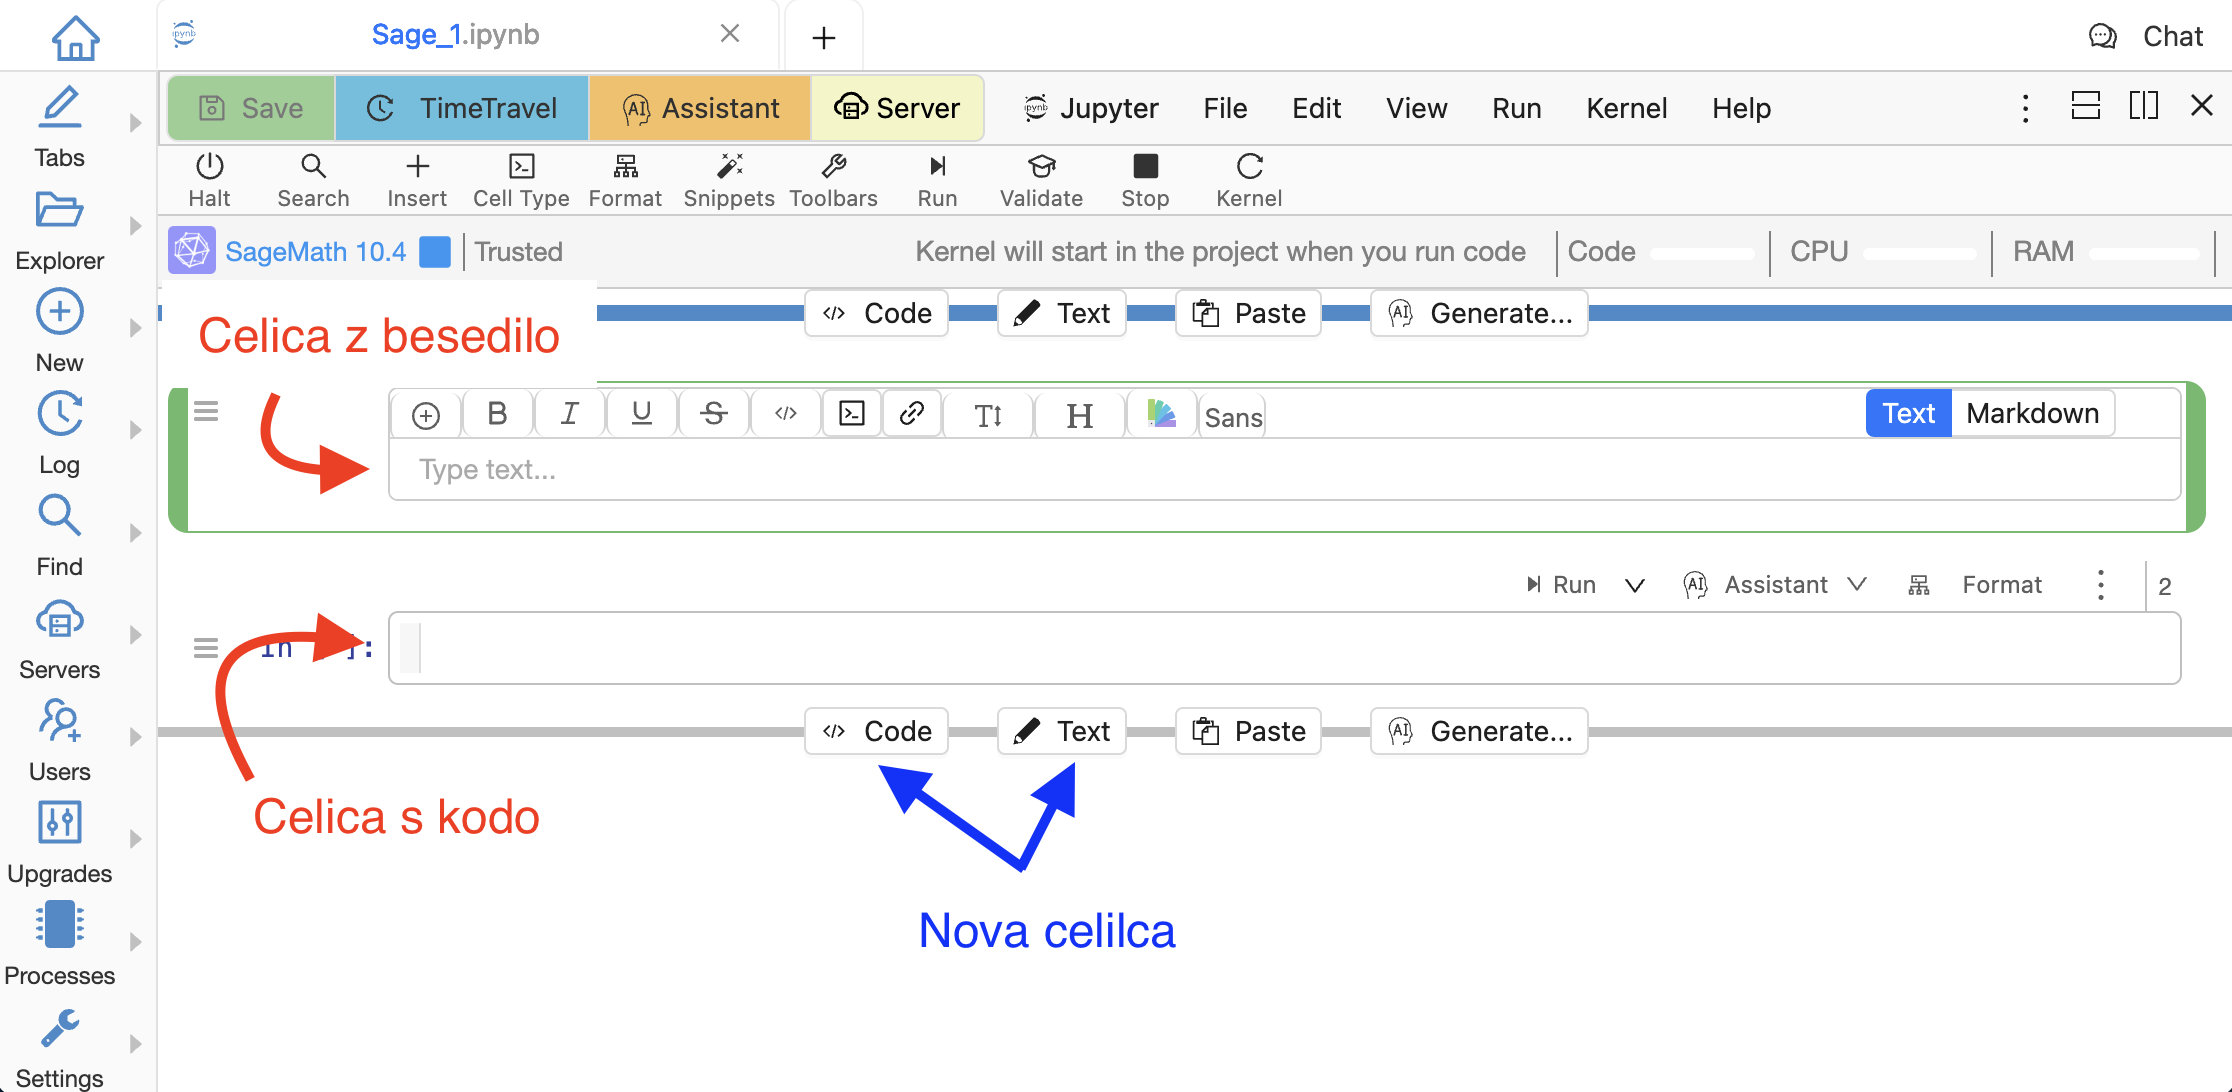
\includegraphics[width=0.5\linewidth]{files/jupyter4-93d3d90c4365029d3ccf05b56075a4ed.png}
\caption[]{Celice v Jupyter}
\label{fig-celice}
\end{figure}

V celici z besedilo lahko uporabite \textit{Markdown} ali standardne besedilo. Priporočamo, da uporabite \textit{Markdown}, saj omogoča boljšo oblikovanje besedila in vključevanje matematičnih izrazov.

\begin{framed}
\textbf{Glej tudi}\\
Markdown je preprost jezik za označevanje besedila, ki omogoča enostavno oblikovanje besedila. Pristop je podoben LaTeX-u, vendar je veliko enostavnejši za uporabo, na žalost, pa tudi manj zmogljiv.

Osnovne značilnosti Markdowna vključujejo:

\begin{itemize}
\item Naslovi: Uporabite \texttt{\# Naslov} za naslove. Več \texttt{\#} pomeni nižjo raven naslova.
\item Krepko in ležeče besedilo: Uporabite \texttt{**krepko**} za \textbf{krepko} besedilo in \texttt{\_ležeče\_} za \textit{ležeče besedilo}.
\item Seznami: Uporabite \texttt{-} ali \texttt{*} za neurejene sezname in številke za urejene sezname.
\item Povezave: Uporabite \texttt{[besedilo](URL)} za ustvarjanje povezav.
\item V Jupyter zvezkih lahko vključite tudi matematični izraze z uporabo LaTeX sintakse, na primer \texttt{\$x\^2 + y\^2 = z\^2\$} za inline izraze in \texttt{\$\$E = mc\^2\$\$} za prikazne izraze.
\end{itemize}

Za več informacij o Markdownu si oglejte naslednje vire: \href{https://www.markdownguide.org/basic-syntax/}{Markdown osnovna sintaksa}

Ta učbenik je napisan v Myst Markdown, ki je razširitev Markdowna.
\end{framed}


\bigskip
\centerline{\rule{13cm}{0.4pt}}
\bigskip

V celici z kodo vnesemo ukaze SageMath. Za izvedbo kode pritisnite  +  ali kliknite na gumb ``Run'' v orodni vrstici. Rezultati se bodo prikazali neposredno pod celico z kodo.

\paragraph{SageMath kot kalkulator}

SageMath lahko uporabljamo kot kalkulator za osnovne aritmetične operacije, kot so seštevanje, odštevanje, množenje in deljenje. Poleg tega lahko uporabljamo tudi bolj zapletene matematične funkcije in operacije.

Z nekaj manjšimi izjemami Sage uporablja programski jezik Python, zato so osnovne aritmetične operacije in druge osnove programiranja v SageMath zelo podobne tistim v Pythonu.

Poglejte naslednje primere. Še bolj pa jih preizkusite sami v svojem CoCalc zvezku!

\begin{verbatim}
1+1
\end{verbatim}

\begin{verbatim}
( 1 + 2 * (3 + 5) ) * 2
\end{verbatim}

Simbol * pomeni množenje, ki se ne sme izpustiti, tudi v izrazih, kot je $2x$: \texttt{2*x}. Za združevanje simbolov uporabljamo oklepaj \texttt{(} \texttt{)} nikoli \texttt{[} \texttt{]} ali \texttt{\{} \texttt{\}}.

\begin{verbatim}
2**3 # ** pomeni potenciranje, kot v Pythonu
\end{verbatim}

\begin{verbatim}
8
\end{verbatim}

\begin{verbatim}
2^3 # ampak ^ pomeni tudi potenciranje, za razliko od Pythona
\end{verbatim}

\begin{verbatim}
-3^2 # pazite!
\end{verbatim}

\begin{verbatim}
-9
\end{verbatim}

Vrstni red izvajanja operacij je določen v \href{https://doc.sagemath.org/html/en/tutorial/appendix.html\#section-precedence}{Arithmetical binary operator precedence}.

\begin{verbatim}
20/6 # Deljenje se označi z /
\end{verbatim}

Pri vzeto SageMath poskuša privzeto vrniti izraz, ki je čim bolj natančen. To je \texttt{10/3} vrne racionalno število $10/3$ (in ne decimalno približek, kot je $3,33333$). Če želimo številčni približek, lahko enemu od števil preprosto dodamo decimalno piko.

\begin{verbatim}
20.0/6
\end{verbatim}

Kvadratne korene lahko izračunamo z ukazom \texttt{sqrt()}. Upoštevajte, da če je argument celo število, SageMath interpretira rezultat kot simbolno število.

\begin{verbatim}
sqrt(2)
\end{verbatim}

\begin{verbatim}
sqrt(2)
\end{verbatim}

\begin{verbatim}
sqrt(8)
\end{verbatim}

Seveda, lahko dobimo številčni približek z ukazom \texttt{sqrt(8.0)}. Na splošno lahko dobimo numerične približke izrazov z (enakovrednimi) ukazi \texttt{n()}, \texttt{N()}, \texttt{numerical\_approx()}. Vsi zgornji ukazi imajo neobvezen argument \texttt{digits} za določitev natančnosti približke.

\begin{verbatim}
n(sqrt(8), digits=50)
\end{verbatim}

V Table~\ref{tab-operacije} so povzete osnovne aritmetične operacije v SageMath-u.

\begin{table}
\centering
\caption[]{Osnovne aritmetične operacije v SageMath-u}
\label{tab-operacije}
\begin{tabular}{p{\dimexpr 0.500\linewidth-2\tabcolsep}p{\dimexpr 0.500\linewidth-2\tabcolsep}}
\toprule
Seštevanje ($a+b$) & \texttt{a+b} \\
Odštevanje ($a -b$) & \texttt{a-b} \\
Množenje ($ab$) & \texttt{a*b} \\
Deljenje ($\frac{a}{b}$) & \texttt{a/b} \\
Potenciranje ($a^b$) & \texttt{a**b} ali \texttt{a\^=b} \\
Kvadratni koren ($\sqrt{a}$) & \texttt{sqrt(a)} \\
Splošni koren ($\sqrt[n]{a}$) & \texttt{a\^(1/n)} \\
\bottomrule
\end{tabular}
\end{table}

\paragraph{Operacije s celimi števili}

S simboli \texttt{//} in \texttt{\%} dobimo (celoštevilski) kvocient oziroma ostanek dveh celih števil

\begin{equation}
20 = 6 \cdot 3 + 2
\end{equation}

\begin{verbatim}
20 // 6
\end{verbatim}

\begin{verbatim}
20 % 6
\end{verbatim}

\begin{verbatim}
divmod(20,6) # vrne kvocient in ostanek hkrati kot tuple
\end{verbatim}

Izračunamo lahko tudi fakultete in binomske koeficiente

\begin{equation}
3!=6
\end{equation}

\begin{verbatim}
factorial(3)
\end{verbatim}

\begin{equation}
\binom{4}{2} = 6
\end{equation}

\begin{verbatim}
binomial(4,2)
\end{verbatim}

Število lahko faktoriziramo kot produkt praštevil

\begin{verbatim}
factor(factorial(7))
\end{verbatim}

Lahko uporabimo naslednji način tudi

\begin{verbatim}
(factorial(7)).factor()
\end{verbatim}

\begin{verbatim}
641 * 6700417
\end{verbatim}

Če želimo vedeti, ali je število praštevilo, lahko uporabimo ukaz \texttt{is\_prime()}:

\begin{verbatim}
is_prime(29)
\end{verbatim}

\begin{verbatim}
is_prime(65537)
\end{verbatim}

Delitelje števila lahko dobimo na naslednji način.

\begin{verbatim}
12.divisors()
\end{verbatim}

Če samo želimo delitelje, ki so praštevila:

\begin{verbatim}
120.prime_divisors()
\end{verbatim}

\begin{verbatim}
120.prime_factors()
\end{verbatim}

Izračunamo lahko \textit{največji skupni delitelj} in \textit{najmanjši skupni večkratnik} dveh števil.

\begin{equation}
D(120,48) =
\end{equation}

\begin{verbatim}
gcd(120,48)
\end{verbatim}

\begin{equation}
v(9,15) =
\end{equation}

\begin{verbatim}
lcm(9,15)
\end{verbatim}

\paragraph{Matematične konstante in funkcije}

Pogoste konstante in funkcije so določene

\begin{equation}
\sin(\pi) = 0
\end{equation}

\begin{verbatim}
sin(pi)
\end{verbatim}

\begin{verbatim}
cos(pi/4)
\end{verbatim}

{\textbackslash}({\textbackslash}displaystyle {\textbackslash}frac\{1\}\{2\} {\textbackslash}, {\textbackslash}sqrt\{2\}{\textbackslash})

Vsak objekt v SageMath-u ima predstavitev LaTeX, ki jo dobimo z ukazom \texttt{latex()}

\begin{verbatim}
latex(cos(pi/4))
\end{verbatim}

{\textbackslash}({\textbackslash}displaystyle {\textbackslash}frac\{1\}\{2\} {\textbackslash}, {\textbackslash}sqrt\{2\}{\textbackslash})

Če želimo da izhod je predstavljen v LaTeX-u, uporabimo čarobni ukaz \texttt{\%display latex}

\begin{verbatim}
%display latex # Ponovno zaženite zgornje primere, potem ko izvedete ta ukaz.
\end{verbatim}

Če želimo vrniti standardni izhod, uporabimo ukaz:

\begin{verbatim}
%display plain
\end{verbatim}

V SageMath lahko delamo tudi z kompleksnimi števili. Imaginarno število $i$ je označeno z \texttt{i} in z \texttt{I}. Ker pa se \texttt{i} pogosto uporablja pri programiranju, je dobra praksa, da se označi z \texttt{I}.

\begin{verbatim}
arg(1+I)
\end{verbatim}

\begin{verbatim}
latex(1+I)
\end{verbatim}

\begin{verbatim}
i + 1
\end{verbatim}

Nekateri viri namesto $e$ raje pišejo $\exp$ in SageMath meni, da je to v redu.

\begin{verbatim}
e^3 - exp(3)
\end{verbatim}

Ukaza \texttt{max()} in \texttt{min()} vrneta največje in najmanjše število v nizu števil.

\begin{verbatim}
max(1,2,3)
\end{verbatim}

\begin{verbatim}
min(1,2,3)
\end{verbatim}

V SageMathu, podobno kot v Pythonu, so seznami zapisani v oklepajih \texttt{[]}

\begin{verbatim}
max([2,3,4,5])
\end{verbatim}

Ukaz \texttt{floor()} zaokroži število navzdol na najbližje celo število, ukaz \texttt{ceil()} pa zaokroži navzgor.

\begin{verbatim}
floor(2.1)
\end{verbatim}

\begin{verbatim}
ceil(2.1)
\end{verbatim}

\textbf{Pazite!}

\begin{verbatim}
floor(1/(2.1 -2))
\end{verbatim}

Ampak
\begin{equation}
\left\lfloor \frac{1}{2.1 - 2} \right\rfloor = \left\lfloor \frac{1}{.1} \right\rfloor = \left\lfloor 10 \right\rfloor = 10
\end{equation}

Kaj se je zgodilo?

Računalniki shranjujejo realna števila v binarni obliki, mi pa smo navajeni uporabljati desetiško predstavitev. Število 2.1 v desetiškem zapisu je precej preprosto in kratko, vendar je po pretvorbi v binarni zapis $10.0\overline{0011} = 10.0001100110011 \dots$

Ker računalniki ne morejo shraniti neskončnega števila številk, se to število nekje zaokroži, kar povzroči manjšo napako, ki smo jo videli.
V SageMathu pa so racionalna števila (ulomki) natančna, zato te napake pri zaokroževanju nikoli ne bomo videli.

\begin{verbatim}
floor(1/ ( (21/10) - 2) )
\end{verbatim}

\subsubsection{Pripisovanje, enakost, enačbe in neenačbe.}

SageMath uporablja \texttt{=} za pripisovanje. Za primerjavo uporablja \texttt{==}, \texttt{\textless =}, \texttt{\textgreater =}, \texttt{\textless } in \texttt{\textgreater }:

\begin{verbatim}
a=5
a
\end{verbatim}

\begin{verbatim}
2 == 2
\end{verbatim}

\begin{verbatim}
2<=3
\end{verbatim}

\begin{verbatim}
2<2
\end{verbatim}

\begin{verbatim}
a < 3
\end{verbatim}

\begin{verbatim}
a == 5
\end{verbatim}

Če želimo shraniti rezultat izračuna, ga dodelimo spremenljivki:

\begin{verbatim}
y=1+2
\end{verbatim}

\textbf{Pazite}: Pogosta napaka je uporaba izraza \texttt{a=b} za primerjavo \texttt{a} in \texttt{b}, vendar na koncu vrednost \texttt{a} zamenjate z vrednostjo \texttt{b}.

\begin{verbatim}
y*(y+2)
\end{verbatim}

Rezultat izračuna se ne natisne samodejno, ko je pripisan spremenljivki.
Zato bomo naredili naslednje, da ga tudi natisnemo,

\begin{verbatim}
b=3*4 ; b
\end{verbatim}

Znak \texttt{;}, ki ločuje več navodil v isti vrstici.
Če ni določeno drugače, se v beležnici Jupyter natisne samo izpis, ki ga ustvari zadnja vrstica. Zato je uporaba znaka \texttt{;} enakovredna uporabi nove vrstice v isti celici.

\begin{verbatim}
y = 3 + 2; y
y+2
\end{verbatim}

Če želimo natisniti vsak korak, moramo uporabiti ukaz \texttt{print()}

\begin{verbatim}
y = 1 + 2; print(y)
y = 3 * y + 1; print(y)
y = 3 * y + 1; print(y)
y = 3 * y + 1; print(y)
\end{verbatim}

\begin{itemize}
\item Če znate programirati v Pythonu, boste morda ugotovili, da je to standardno obnašanje spremenljivke.
\end{itemize}

\begin{itemize}
\item Ni priporočljivo na novo definirati vnaprej določenih konstant in funkcij iz programa Sage.
\item Čeprav to ne vpliva na notranje obnašanje programa Sage, lahko privede do presenetljivih rezultatov:
\end{itemize}

\begin{verbatim}
pi = -I/2
\end{verbatim}

\begin{verbatim}
exp(2*I*pi)
\end{verbatim}

Ukaz \texttt{restore()} povrne privzeto vrednost vsem vnaprej določenim spremenljivkam in funkcijam.

\begin{verbatim}
restore()
\end{verbatim}

\begin{verbatim}
y+pi
\end{verbatim}

Ukaz \texttt{reset()} opravi še popolnejšo ponastavitev, zlasti izbriše vse uporabniško definirane spremenljivke.

\begin{verbatim}
reset()
\end{verbatim}

\begin{verbatim}
y
\end{verbatim}

Opazite tudi, da SageMath včasih razlikuje med simbolnimi izračuni in števili.

\begin{verbatim}
e^(2*pi*I)
\end{verbatim}

\begin{verbatim}
e^(2*pi*I) == 1
\end{verbatim}

SageMath zgornjega ne razume kot primerjavo, temveč kot enačbo.

\begin{verbatim}
3*x - 10 == 5
\end{verbatim}

Enačbo ali neenakost rešimo z ukazom \texttt{solve()}.

\begin{verbatim}
solve(3*x - 2 == 5,x)
\end{verbatim}

Privzeto SageMath interpretira \texttt{x} kot simbolno spremenljivko. Za zdaj bomo reševali samo \texttt{x}, pozneje pa bomo videli, kako določiti lastne (simbolne) spremenljivke

\begin{verbatim}
solve( 2*x - 5 >= 17,x)
\end{verbatim}

\begin{verbatim}
solve( x^2 + x == 6, x)
\end{verbatim}

\begin{verbatim}
solve(2*x^2 - x + 1 == 0, x)
\end{verbatim}

Množica rešitev nekaterih neenačb je sestavljena iz unije in preseka odprtih intervalov.

\begin{verbatim}
solve( x^2 - 6 >= 3, x )
\end{verbatim}

\begin{verbatim}
solve( x^2 - 6 <= 3, x )
\end{verbatim}

\begin{itemize}
\item Ukaz \texttt{solve()} poskuša izraziti rešitev enačbe brez uporabe števil s plavajočo vejico.
\item Če tega ni mogoče storiti, bo vrnil rešitev v simbolični obliki.
\end{itemize}

\begin{verbatim}
solve( sin(x) == x, x)
\end{verbatim}

\begin{itemize}
\item Za iskanje numeričnega približka rešitve lahko uporabimo ukaz \texttt{find\_root()}.
\item Ta ukaz zahteva izraz in zaprt interval, na katerem se išče rešitev
\end{itemize}

\begin{verbatim}
find_root(sin(x) == x, -pi/2 , pi/2)
\end{verbatim}

\begin{itemize}
\item Ob začetku seje SageMath ustvari eno simbolno spremenljivko, \texttt{x}, ki se lahko uporablja za reševanje enačb.
\item Če želite uporabiti dodatno simbolno spremenljivko, jo morate deklarirati z ukazom \texttt{var()}.
\end{itemize}

\begin{verbatim}
y,z,t = var("y z t")
\end{verbatim}

\begin{verbatim}
phi, theta, rho = var("phi theta rho")
\end{verbatim}

\begin{verbatim}
x1, x2 = var("x1 x2")
\end{verbatim}

\begin{itemize}
\item Imena spremenljivk ne smejo vsebovati presledkov
\item Na primer \texttt{square root} ni veljavno ime spremenljivke, \texttt{square\_root} pa je.
\end{itemize}

Poskus uporabe simbolne spremenljivke, preden je bila deklarirana, bo povzročil napako \texttt{NameError}.

\begin{verbatim}
u
\end{verbatim}

\begin{verbatim}
solve (u^2 -1,u)
\end{verbatim}

Simbolno spremenljivko, kot je zgoraj opredeljena spremenljivka \texttt{phi}, lahko razglašamo z ukazom \texttt{restore()}.

\begin{verbatim}
restore('phi')
\end{verbatim}

\begin{verbatim}
phi
\end{verbatim}

Majhne sisteme linearnih enačb lahko rešite tudi s ukazom \texttt{solve()}, če imajo vse simbolne spremenljivke so bile deklarirane.

\begin{verbatim}
x,y,z = var('x','y','z')
\end{verbatim}

\begin{verbatim}
solve( [3*x - y == 2, -2*x -y == 1 ], x,y)
\end{verbatim}

\begin{verbatim}
[[x == (1/5), y == ( -7/5)]]
\end{verbatim}

\begin{verbatim}
solve( [ 2*x - y == -1 , 2*x - y == 2],x,y)
\end{verbatim}

\begin{verbatim}
solve( [ 2*x + y == -1 , -4*x - 2*y == 2],x,y)
\end{verbatim}

\begin{itemize}
\item \texttt{r1} označuje, da obstaja prosta spremenljivka, ki določa množico rešitev.
\end{itemize}

\begin{itemize}
\item Če je več prostih spremenljivk, jih SageMath našteje \texttt{r1,r2,..., rk}.
\end{itemize}

\begin{verbatim}
solve([ 2*x + 3*y + 5*z == 1, 4*x + 6*y + 10*z == 2, 6*x + 9*y + 15*z == 3], x,y,z)
\end{verbatim}

\begin{verbatim}
[[x == -5/2*r3 - 3/2*r4 + 1/2, y == r4, z == r3]]
\end{verbatim}

\begin{itemize}
\item Ukaz \texttt{solve()} je lahko pri velikih sistemih enačb zelo počasen.
\item Za te sisteme je najbolje uporabiti funkcije linearne algebre, saj so precej učinkovite. Kmalu se bomo naučili, kako.
\end{itemize}

Reševanje neenačb v več spremenljivkah lahko privede do zapletenih izrazov, saj so območja, ki jih določajo, zapletena.

\begin{verbatim}
solve([ x -y >=2, x+y <=3], x,y)
\end{verbatim}

\subparagraph{Vaje}

\begin{enumerate}
\item Poiščite vse rešitve enačbe $x^{3} - x = 7x^{2} -7$
\item Poišči celotno množico rešitev za neenačbo $|t -7| \geq 3$
\item Poiščite vsa $x$ in $y$, ki izpolnjujejo tako $2x+ y= 17$ kot $x -3y= -16$.
\item S funkcijo \texttt{find\_root()} poiščite rešitev enačbe $e^{x} = \cos(x)$ na intervalu $[ -\pi/2,0]$.
\item Zgornji ukaz spremenite tako, da find\_root()najde drugo rešitev na istem intervalu.
\end{enumerate}

\subsubsection{Lepe praznike!}

\begin{verbatim}
var('t k')
from sage.plot.plot3d.shapes import *
num_wraps=4
num_lights=30
c=rainbow(num_lights)
f(t) = ( (1 -t)*cos(2*pi*t*num_wraps), (1 -t)*sin(2*pi*t*num_wraps),t)
lights=add([point(f(1/(num_lights)*(k+1)),color=c[k],size=50) for k in range(0,num_lights)])
S = Cone(1, 1, color='green')
S += parametric_plot3d(f(t),(t,0,1),thickness=3  )
S += lights
S.show(frame=false)
\end{verbatim}

\subsection{Algebra s SageMath}

V izdelavi.

\subsection{Sage: Analiza in risanje grafov.}

V izdelavi.

\section{Priloge}

\subsection{Nameščanje LaTeXa na svoj računalnik}

LaTeX je popolnoma brezplačen in ga lahko enostavno namestite na svoj računalnik.
Uradno spletno stran za namestitev si lahko ogledate \href{https://www.latex-project.org/get/}{tukaj} (v angleščini).

Za uporabo LaTeXa potrebujete v bistvu dve orodji:

\begin{itemize}
\item distribucijo LaTeX, ki je sam program LaTeX, s katerim boste ustvarjali svoje dokumente.
\item urejevalnik besedil, ki je vmesnik, ki ga boste uporabljali za pisanje in izdelavo dokumentov. Verjetno že imate urejevalnik besedil na svojem računalniku (npr. Notepad ali TextEdit). Ti urejevalniki so večnamenski in imajo običajno zelo malo orodij. Na tej strani priporočamo nekaj možnosti, ki vam bodo olajšale delo.
\end{itemize}

\subsubsection{Windows}

\paragraph{Namestitev distribucije}

\begin{enumerate}
\item Odprite spletno stran \href{https://miktex.org/download}{MiKTeX}.
\item Prenesite namestitveni program za Windows.
\item Zaženite namestitev in sledite navodilom (pustite privzete nastavitve).
\item Po zaključku preverite namestitev tako, da v ukazni vrstici (Command Prompt) vpišete:

\begin{verbatim}
pdflatex - -version
\end{verbatim}
\end{enumerate}

\paragraph{Priporočeni urejevalniki}

\begin{itemize}
\item \href{https://code.visualstudio.com/}{Visual Studio Code} (potrebujete tudi razširitev \textit{LaTeX Workshop}). Še bolje, predlagamo, da namestite \href{https://vscodium.com/}{VSCodium}, brezplačno/odprtokodno različico vscode.
\item \href{https://www.tug.org/texworks/}{TeXworks} (preprost, pogosto nameščen z MiKTeX).
\item \href{https://www.texstudio.org/}{TeXstudio} (bolj napreden, uporabniku prijazen).
\end{itemize}

\subsubsection{macOS}

\paragraph{Namestitev distribucije}

\begin{enumerate}
\item Odprite spletno stran \href{https://tug.org/mactex/}{MacTeX}.
\item Prenesite paket \textbf{MacTeX.pkg} (velik {\textasciitilde}4 GB).
\item Odprite preneseno datoteko in sledite navodilom za namestitev.
\item Preverite namestitev v Terminalu:

\begin{verbatim}
pdflatex - -version
\end{verbatim}
\end{enumerate}

\paragraph{Priporočeni urejevalniki}

\begin{itemize}
\item \href{https://code.visualstudio.com/}{Visual Studio Code} (razširitev \textit{LaTeX Workshop}).
Še bolje, predlagamo, da namestite \href{https://vscodium.com/}{VSCodium}, brezplačno/odprtokodno različico vscode.
\item \href{https://pages.uoregon.edu/koch/texshop/}{TeXShop} (priložen MacTeX-u).
\item \href{https://www.texstudio.org/}{TeXstudio}.
\end{itemize}

\subsubsection{Linux (primer: Ubuntu/Debian)}

Če uporabljate Linux, verjetno ne potrebujete naših navodil.

\paragraph{Namestitev distribucije}

\begin{enumerate}
\item Odprite Terminal.
\item Namestite TeX Live:

\begin{verbatim}
sudo apt update
sudo apt install texlive -full
\end{verbatim}


\item Preverite namestitev:

\begin{verbatim}
pdflatex - -version
\end{verbatim}
\end{enumerate}

\paragraph{Priporočeni urejevalniki}

\begin{itemize}
\item \href{https://code.visualstudio.com/}{Visual Studio Code}. (razširitev \textit{LaTeX Workshop}). Še bolje, predlagamo, da namestite \href{https://vscodium.com/}{VSCodium}, brezplačno/odprtokodno različico vscode.
\item \href{https://kile.sourceforge.io/}{Kile} (posebej priljubljen v Linux okolju).
\item \href{https://www.texstudio.org/}{TeXstudio}.
\item \href{https://www.tug.org/texworks/}{TeXworks}.
\end{itemize}

\subsection{Izvoz datotek iz Overleaf projekta}

Če želite izvoziti celoten projekt iz Overleafa kot \texttt{.zip} ali \texttt{pdf} datoteko, sledite naslednjim korakom:

\begin{enumerate}
\item \textbf{Odprite projekt} v Overleafu, iz katerega želite prenesti datoteke.
\item V zgornjem levem kotu kliknite na gumb \textbf{Menu}.
\item V spustnem meniju izberite možnost \textbf{Download \textgreater  Source} (če želite \texttt{.zip} datoteko) ali \textbf{Download \textgreater  PDF} (če želite \texttt{.pdf} dokument).
\item Overleaf bo ustvaril in prenesel \texttt{.zip} datoteko, ki vsebuje vse datoteke projekta (npr. \texttt{.tex} datoteke, slike, \texttt{.bib} datoteke, ipd.) oziroma \texttt{.pdf} dokument.
\item Shrani preneseno datoteko na svoj računalnik in jo po potrebi razširi.
\end{enumerate}

\subsection{Dolžine v LaTeXu}

Dolžine (\textit{lengths}) so pomemben del LaTeXa, saj omogočajo natančen nadzor nad razmikom, velikostjo elementov, zamiki, robovi in še več.
Vsaka dolžina je shranjena kot spremenljivka, ki ji lahko dodelimo vrednost, jo povečamo ali zmanjšamo, in uporabimo pri različnih ukazih.

\subsubsection{Osnovne merske enote}

V LaTeXu lahko dolžine izrazimo z različnimi enotami. Najpogosteje uporabljene so:

\bigskip\noindent
\begin{tabular}{p{\dimexpr 0.500\linewidth-2\tabcolsep}p{\dimexpr 0.500\linewidth-2\tabcolsep}}
\toprule
Enota & Opis \\
\hline
\texttt{pt} & točka (1/72,27 palca) -- osnovna enota v TeXu \\
\texttt{mm} & milimeter \\
\texttt{cm} & centimeter \\
\texttt{in} & palec (2.54 cm) \\
\texttt{ex} & višina male črke \textit{x} v trenutni pisavi \\
\texttt{em} & širina črke \textit{M} v trenutni pisavi \\
\texttt{bp} & velika točka (1/72 palca) \\
\texttt{pc} & pica = 12 točk \\
\texttt{dd} & didotova točka \\
\texttt{cc} & cicer = 12 didotov \\
\texttt{sp} & najmanjša notranja enota v TeXu (65536 sp = 1 pt) \\
\bottomrule
\end{tabular}

\bigskip\subsubsection{Privzete dolžinske spremenljivke}

LaTeX ima več že vnaprej določenih dolžin, ki vplivajo na izgled dokumenta:

\bigskip\noindent
\begin{tabular}{p{\dimexpr 0.500\linewidth-2\tabcolsep}p{\dimexpr 0.500\linewidth-2\tabcolsep}}
\toprule
Dolžina & Opis \\
\hline
\texttt{{\textbackslash}textwidth} & širina glavnega besedila \\
\texttt{{\textbackslash}textheight} & višina glavnega besedila \\
\texttt{{\textbackslash}linewidth} & širina vrstice znotraj okolja (npr. v \texttt{minipage}) \\
\texttt{{\textbackslash}columnwidth} & širina stolpca v dvostolpčnem načinu \\
\texttt{{\textbackslash}paperwidth}, \texttt{{\textbackslash}paperheight} & dimenzije papirja \\
\texttt{{\textbackslash}parindent} & zamik prve vrstice odstavka \\
\texttt{{\textbackslash}parskip} & razmik med odstavki \\
\texttt{{\textbackslash}baselineskip} & navpična razdalja med vrsticami besedila \\
\texttt{{\textbackslash}topmargin}, \texttt{{\textbackslash}oddsidemargin}, \texttt{{\textbackslash}evensidemargin} & robovi strani \\
\bottomrule
\end{tabular}

\bigskip
%  Primer uporabe:
% 
% ```latex
% \setlength{\parindent}{0pt}
% \setlength{\parskip}{1em}
% ```
% 
% S tem odstranimo zamik odstavkov in dodamo več prostora med njimi.
% 
% ## Določanje in spreminjanje dolžin
% 
% Za delo z dolžinami uporabljamo naslednje ukaze:
% 
% ```latex
% \setlength{\ime}{vrednost}
% \addtolength{\ime}{vrednost}
% ```
% 
% Primer:
% 
% ```latex
% \setlength{\textwidth}{14cm}
% \addtolength{\textwidth}{1cm}
% ```
% 
% Ukaz `\setlength` nastavi absolutno vrednost, medtem ko `\addtolength` doda (ali odšteje) določeno dolžino.
% 
% ## Uporaba dolžin v izrazih
% 
% LaTeX omogoča uporabo relativnih vrednosti in računanje z dolžinami z uporabo ukaza `\dimexpr`. Primer:
% 
% ```latex
% \setlength{\textwidth}{\dimexpr\paperwidth-2in\relax}
% ```
% 
% Ta ukaz nastavi širino besedila tako, da je za 2 palca manjša od širine papirja.

%  ## Uporabni namigi
% 
% - Dolžine lahko definirate tudi sami z `\newlength`:
%   ```latex
%   \newlength{\mojadolzina}
%   \setlength{\mojadolzina}{5cm}
%   ```
% - Za začasne spremembe uporabite okolje `minipage`, kjer lahko lokalno spremenite `\linewidth`.
% - Za bolj napreden nadzor nad postavitvijo lahko uporabite pakete kot so `geometry`, `calc` ali `layouts`.





\end{document}
